%\documentclass[a4papper, 12pt, titlepage]{book}
\documentclass[a4papper, 12pt]{book}

\usepackage[utf8]{inputenc}
\usepackage[T1]{fontenc}
\usepackage[normalem]{ulem}
\usepackage[francais,english]{babel}% langue principale = english
\usepackage{graphicx}
\usepackage{caption}
\usepackage{subcaption}
%\usepackage{a4wide}
\usepackage{ulem}
\usepackage{enumerate}
\usepackage{array}
\usepackage{amsmath}
\usepackage{amssymb}
\usepackage{mathrsfs}
\usepackage{textcomp}
\usepackage{mathtools}
\usepackage{verbatim}
\usepackage{listings}
\usepackage{url}
\usepackage{moreverb}
\usepackage{placeins} 
\usepackage[table]{xcolor}
\usepackage{array,multirow,makecell}
\usepackage[tight]{shorttoc}
\usepackage{lettrine}
\usepackage{oldgerm}
\usepackage{import}
\usepackage{hyperref}
\usepackage{todonotes}
\usepackage{minitoc}
\usepackage{helvet}

\hypersetup{
  backref=true, %permet d'ajouter des liens dans... pagebackref=true,%...les bibliographies
  hyperindex=true, %ajoute des liens dans les index.
  colorlinks=true, %colorise les liens
  breaklinks=true, %permet le retour à la ligne dans les liens trop longs urlcolor= blue, %couleur des hyperliens
  linkcolor= blue, %couleur des liens internes
  bookmarks=true, %créé des signets pour Acrobat
  bookmarksopen=true,
  pdftitle={Intelligent detection layers for tracking in high energy physics}, 
  pdfauthor={Benjamin BOITRELLE},
  pdfsubject={Mac OS X}
}

\newcommand{\sommaire}{\shorttoc{Sommaire}{1}}

% \usepackage{fullpage}
\usepackage[nottoc, notlof, notlot]{tocbibind}
\usepackage[toc,acronym,nomain,indexonlyfirst]{glossaries}

%\usepackage{geometry}
%\geometry{hmargin=2.5cm}

 \definecolor{light-gray}{gray}{0.85}
 %\newcolumntype{M}[1]{>{\raggedright}m{#1}}
 \newcolumntype{M}[1]{>{\centering\arraybackslash}m{#1}} % To center text in table
 
\renewcommand{\baselinestretch}{0.9}
%\newcommand{\noyau}[3]{\prescript{#2}{#3}{\mathrm{#1}}}

\lstset{language=c++,numbers=left,tabsize=2,breaklines=true}

\makeatletter
\def\clap#1{\hbox to 0pt{\hss #1\hss}}%
\def\ligne#1{%
    \hbox to \hsize{%
\vbox{\centering #1}}}%
\def\haut#1#2#3{%
    \hbox to \hsize{%
        \rlap{\vtop{\raggedright #1}}%
        \hss
        \clap{\vtop{\centering #2}}%
        \hss
\llap{\vtop{\raggedleft #3}}}}%
\def\bas#1#2#3{%
    \hbox to \hsize{%
        \rlap{\vbox{\raggedright #1}}%
        \hss
        \clap{\vbox{\centering #2}}%
        \hss
\llap{\vbox{\raggedleft #3}}}}%
\def\maketitle{%
    \thispagestyle{empty}\vbox to \vsize{%
        \haut{}{\@blurb}{}
        \vfill
        \vspace{3cm}
        \begin{center}
            \usefont{OT1}{ptm}{m}{n}
            \huge \@title
        \end{center}
        \par
        \hrule height 4pt
        \par
        \begin{flushright}
            \usefont{OT1}{phv}{m}{n}
            \Large \@author
            \par
        \end{flushright}
        \vspace{1cm}
        \vfill
        \vfill
        \bas{}{\@location, \@date}{}
        \vspace{1cm}
        %\includegraphics[scale = 0.1]{Logos/LogoUCBL}
        %\hfill
        %\includegraphics[scale = 0.2]{Logos/logo_IPHC_10cm}
        %\hfill
        %\includegraphics[scale = 0.15]{Logos/CNRS_logo}
        %\hfill
    }%
    \cleardoublepage
}
\def\date#1{\def\@date{#1}}
\def\author#1{\def\@author{#1}}
\def\title#1{\def\@title{#1}}
\def\location#1{\def\@location{#1}}
\def\blurb#1{\def\@blurb{#1}}
\date{}
\author{}
\title{}
\location{DESY - Hamburg}\blurb{}
\makeatother
\title{Intelligent detection layers for tracking in high energy physics}
\author{Benjamin \textsc{Boitrelle}}

\location{DESY - Hamburg}
%\blurb{%
%    Université de Strasbourg\\
%    École Doctorale de Physique et Chimie-Physique (ED182) \\ 
%    \textbf{Thèse}\\[1em]
%Directeur de thèse : Jérôme \textsc{Baudot}\\ % 
%Co-directeur de thèse : Ingrid \textsc{Maria Gregor}\\ }% 

\makeglossaries
\setacronymstyle{long-short}
\renewcommand*{\glslinkcheckfirsthyperhook}{% To make a reference only for the first glossary entry
  \ifglsused{\glslabel}%
  {%
    \setkeys{glslink}{hyper=false}%
  }%
  {}%
}
\renewcommand*{\glstextformat}[1]{\textcolor{black}{#1}} % To make glossary black and not blue

\newcommand*{\glswriteentry}[2]{%  
  \ifglsindexonlyfirst  
    \ifglsused{#1}{}{#2}%  
  \else  
    #2%  
  \fi  
}
\setlength{\parskip}{1ex plus 0.5ex minus 0.2ex}

\begin{document}

    %\frontmatter
    %\maketitle
    \input{aknowledgements.tex}
    %\setcounter{page}{1}

    \dominitoc
    \tableofcontents
    \listoffigures
    \listoftables
    \listoftodos
%	\sommaire
	
    \mainmatter

    %\chapter*{Introduction\markboth{Introduction}{Introduction}}
\addstarredchapter{Introduction}

  In 2012, the \gls{LHC} detected a new particle compatible with the boson predicted by the Higgs-Englert-Brout mechanism, which explains the spontaneous electro-weak symmetry breaking among elementary interactions.
  Although the energy and luminosity upgrades could improve the knowledge of this new particle and also find existence of physics beyond the \gls{SM}, the complex environment of the events generated by the \gls{LHC} hides fundamental parameters of the collisions that help to perform precise measurements.

  To overcome this limitation and complement the \gls{LHC} programme, one of the biggest scientific projects is under preparation. 
  The \gls{ILC} will be a linear eletron-positron collider with a length of 31 kilometres and a centre-of-mass energy ranging from  $250$ to $500~\rm{GeV}$ (with a possible upgrade to $1~\rm{TeV}$). 
  It will be able to perform more accurate measurements of known particles (like the coupling of the Higgs boson to fermions), but also to study the dark matter and physics beyond the \gls{SM}. 
  
  This project imposes new challenges on the instrumentation side. 
  For instance, to measure the Higgs coupling to charm quarks, a precise measurement of the secondary vertices created close to the interaction point is needed.
  The inner part of the detector used to reconstruct vertices, should combine a good spatial resolution ($\leq 3~\rm{\mu m}$) and a material budget of less than a thousandth of the radiation length ($\rm{X_0}$).
  This subdetector, called the vertex detector, should be optimised (geometry, granularity, timing) to perform tracking in a high particle density environment.
  
  The \gls{PLUME} collaboration is developing devices to overcome this challenge thanks to an innovative concept of double-sided detection layers.
  Two families of prototypes have been built.
  Both exploit the \gls{CMOS} technology for the pixel senors which cover each side of the device layer.
  They differ by their material budget.
  While the first prototype focus on the electric functionality, the second prototype targets a material budget of $0.35~\%$ radiation length ($\rm{X_{0}}$).
  The main purpose of this work is to validate the benefits of \gls{PLUME} concept and characterise the performances of the prototypes in terms of spatial resolution, angular resolution and confirm their actual material budget.
  
  %This detector is equipped with six \gls{CMOS} pixels sensors, placed next to each other on each side of a very lightweight mechanical structure. 
  %The collaboration tries to reach a material budget close to $0.35~\%~\rm{X_0}$. 
  %For each track, two positions will be measured, one on each side. 
  %This double-measurement will help to determine the intersection point of the particle with the detector, but also to estimate the origin and the momentum of the particles.

  This work gives an overview of the validation and characterisation of such a complex detector and aims to detail its performance, such as the spatial resolution, the benefits of double-sided measurements and confirmed the actual the material budget of such a device.
  This document is organised as followed:
  the theoretical context is presented in chapter~\ref{chap:SM}, with an overview of the \gls{SM} and theories beyond the \gls{SM}.
  %Chapter~\ref{chap:SM} presents the theoretical context, with an overview of the \gls{SM} and theories beyond the \gls{SM}.
  Chapter~\ref{chap:ILC} presents the future linear collider, the \gls{ILC} focusing especially on one of the experiments, the \gls{ILD}.
  Chapter~\ref{chap:phyics} introduces the different physics studies that will be performed at the \gls{ILC} and focus especially on a possible analysis of the $\nu\overline{\nu}H$ channel at the \gls{ILC}.
  In chapter~\ref{chap:vxd}, the different \gls{VXD} for the \gls{ILD} are presented, as well as a description of the \gls{PLUME} collaboration and the status of the detectors produced.
  The three last chapters are devoted to the studies performed during this thesis.
  In chapter~\ref{chap:labTests}, the validation in the laboratory of the different \gls{PLUME} modules are reported.
  Chapter~\ref{chap:deformation} presents the observation of the ladder deformation during a test beam campaign which was done in 2011 at \gls{CERN}. 
  It also shows the benefits of a double-sided measurement compared to a single-sided ladder.
  Chapter~\ref{chap:X0} deals with the measurement of the radiation length of the first fully working \gls{PLUME} ladder, which has a weighted material budget ($\rm{X_0}$) estimated to be $0.65~\%~\rm{X_0}$.
  Finally, the conclusion summarises the work performed during the thesis and the outlook is discussed.

%    \chapter*{Introduction\markboth{Introduction}{Introduction}}
\addstarredchapter{Introduction}

  In 2012, the \gls{LHC} detected a new particle compatible with the boson predicted by the Higgs-Englert-Brout mechanism, which explains the spontaneous electro-weak symmetry breaking among elementary interactions.
  Although the energy and luminosity upgrades could improve the knowledge of this new particle and also find existence of physics beyond the \gls{SM}, the complex environment of the events generated by the \gls{LHC} hides fundamental parameters of the collisions that help to perform precise measurements.

  To overcome this limitation and complement the \gls{LHC} programme, one of the biggest scientific projects is under preparation. 
  The \gls{ILC} will be a linear eletron-positron collider with a length of 31 kilometres and a centre-of-mass energy ranging from  $250$ to $500~\rm{GeV}$ (with a possible upgrade to $1~\rm{TeV}$). 
  It will be able to perform more accurate measurements of known particles (like the coupling of the Higgs boson to fermions), but also to study the dark matter and physics beyond the \gls{SM}. 
  
  This project imposes new challenges on the instrumentation side. 
  For instance, to measure the Higgs coupling to charm quarks, a precise measurement of the secondary vertices created close to the interaction point is needed.
  The inner part of the detector used to reconstruct vertices, should combine a good spatial resolution ($\leq 3~\rm{\mu m}$) and a material budget of less than a thousandth of the radiation length ($\rm{X_0}$).
  This subdetector, called the vertex detector, should be optimised (geometry, granularity, timing) to perform tracking in a high particle density environment.
  
  The \gls{PLUME} collaboration is developing devices to overcome this challenge thanks to an innovative concept of double-sided detection layers.
  Two families of prototypes have been built.
  Both exploit the \gls{CMOS} technology for the pixel senors which cover each side of the device layer.
  They differ by their material budget.
  While the first prototype focus on the electric functionality, the second prototype targets a material budget of $0.35~\%$ radiation length ($\rm{X_{0}}$).
  The main purpose of this work is to validate the benefits of \gls{PLUME} concept and characterise the performances of the prototypes in terms of spatial resolution, angular resolution and confirm their actual material budget.
  
  %This detector is equipped with six \gls{CMOS} pixels sensors, placed next to each other on each side of a very lightweight mechanical structure. 
  %The collaboration tries to reach a material budget close to $0.35~\%~\rm{X_0}$. 
  %For each track, two positions will be measured, one on each side. 
  %This double-measurement will help to determine the intersection point of the particle with the detector, but also to estimate the origin and the momentum of the particles.

  This work gives an overview of the validation and characterisation of such a complex detector and aims to detail its performance, such as the spatial resolution, the benefits of double-sided measurements and confirmed the actual the material budget of such a device.
  This document is organised as followed:
  the theoretical context is presented in chapter~\ref{chap:SM}, with an overview of the \gls{SM} and theories beyond the \gls{SM}.
  %Chapter~\ref{chap:SM} presents the theoretical context, with an overview of the \gls{SM} and theories beyond the \gls{SM}.
  Chapter~\ref{chap:ILC} presents the future linear collider, the \gls{ILC} focusing especially on one of the experiments, the \gls{ILD}.
  Chapter~\ref{chap:phyics} introduces the different physics studies that will be performed at the \gls{ILC} and focus especially on a possible analysis of the $\nu\overline{\nu}H$ channel at the \gls{ILC}.
  In chapter~\ref{chap:vxd}, the different \gls{VXD} for the \gls{ILD} are presented, as well as a description of the \gls{PLUME} collaboration and the status of the detectors produced.
  The three last chapters are devoted to the studies performed during this thesis.
  In chapter~\ref{chap:labTests}, the validation in the laboratory of the different \gls{PLUME} modules are reported.
  Chapter~\ref{chap:deformation} presents the observation of the ladder deformation during a test beam campaign which was done in 2011 at \gls{CERN}. 
  It also shows the benefits of a double-sided measurement compared to a single-sided ladder.
  Chapter~\ref{chap:X0} deals with the measurement of the radiation length of the first fully working \gls{PLUME} ladder, which has a weighted material budget ($\rm{X_0}$) estimated to be $0.65~\%~\rm{X_0}$.
  Finally, the conclusion summarises the work performed during the thesis and the outlook is discussed.

    \newacronym{SM}{SM}{Standard Model}
\newacronym{LHC}{LHC}{Large Hadron Collider}
\newacronym{LEP}{LEP}{Large Electron Positron collider}
\newacronym{ILD}{ILD}{International Large Detector}
\newacronym{SiD}{SiD}{Silicon Detector}
\newacronym{PFA}{PFA}{Particle Flow Algorithm}
\newacronym{TPC}{TPC}{Time-Projection-Chamber}
\newacronym{ILC}{ILC}{International Linear Collider}
\newacronym{CLIC}{CLIC}{Compact LInear Collider}
\newacronym{SRF}{SRF}{Superconducting Radio-Frequency}
\newacronym{DC}{DC}{Direct-current}
\newacronym{BDS}{BDS}{Beam Delivery System}
\newacronym{RTML}{RTML}{Ring To the Main Linac}
\newacronym{IR}{IR}{interaction region}
\newacronym{IP}{IP}{interaction point}
\newacronym{VXD}{VXD}{Vertex Detector}
\newacronym{SIT}{SIT}{Silicon Internal Tracker}
\newacronym{SET}{SET}{Silicon External Tracking}
\newacronym{ETD}{ETD}{End-cap Tracking Detector}
\newacronym{FTD}{FTD}{Forward Tracking Detector}
\newacronym{ECAL}{ECAL}{Electromagnetic CALorimeter}
\newacronym{HCAL}{HCAL}{HAdronic CALanalogue HCALorimeter}
\newacronym{AHCAL}{AHCAL}{Analogue HCAL}
\newacronym{SDHCAL}{SDHCAL}{Semi-Digital HCAL}
\newacronym{GRPC}{GRPC}{Glass Resistive Plate Chamber}
\newacronym{LHCAL}{LHCAL}{Low angle Hadron CALorimeter}
\newacronym{PLUME}{PLUME}{Pixelated Ladder with Ultra-low Material Embedding}
\newacronym{CMOS}{CMOS}{Complementary Metal Oxide Semi-conductor}
\newacronym{FPCCD}{FPCCD}{Fine Pixels Charged Coupled-Device}
\newacronym{CCD}{CCD}{Charged Coupled-Device}
\newacronym{ASIC}{ASIC}{Application-Specified Integrated Circuit}
\newacronym{DEPFET}{DEPFET}{Depleted P- Channel Field Effect Transistor}
\newacronym{MIMOSA}{MIMOSA}{Minimum Ionizing MOS Active pixel sensor}
\newacronym{APS}{APS}{Active Pixel Sensor}
\newacronym{MAPS}{MAPS}{Monolithic Active Pixel Sensor}
\newacronym{MIP}{MIP}{Minimum Ionizing Particle}
\newacronym{DAQ}{DAQ}{Data AcQuisition}
\newacronym{FPN}{FPN}{Fixed Pattern Noise}
\newacronym{TN}{TN}{Temporal Noise}
\newacronym{SiC}{SiC}{Silicon Carbide}
\newacronym{OKF}{OKF}{Optiprint-Kapton-Flex-cable}
\newacronym{JTAG}{JTAG}{Joint Test Action Group}
\newacronym{ZIF}{ZIF}{Zero Insertion Force}
\newacronym{SUZE}{SUZE}{Suppression de zéro}
\newacronym{CDS}{CDS}{Correlated Double Sampling}
\newacronym{SNR}{SNR}{Signal to Noise ratio}
\newacronym{TAF}{TAF}{TAPI Analysis Framework}
\newacronym{LCIO}{LCIO}{Linear Collider I/O}
\newacronym{Marlin}{Marlin}{Modular Analysis and Reconstruction for the LINear collider}
\newacronym{GEAR}{GEAR}{GEometry Api for Reconstruction}
\newacronym{ISR}{ISR}{Initial State Radiation}


    \chapter{The secrets of nature}
\label{chap:SM}

\newacronym{SM}{SM}{Standard Model}
\newacronym{EM}{EM}{electromagnetic interaction}

    In this chapter, we will try to understand the world surrounding us thanks to a mathematical framework which describes the matter and its interaction.
    We will first have a look at the laws that lead our Universe. Then, we will focus on the mathematical framework with the description of three interactions: the electromagnetism, the weak and the strong interactions.
    After that, we will study the electroweak interaction and the spontaneous symmetry breaking. We will finally discuss the limits of the theory and the solutions to avoid the limits. 
 \minitoc
 \clearpage
  \section{The Standard Model}

    \subsection{Introduction}
     
    \begin{figure}[!h]
    \centering
      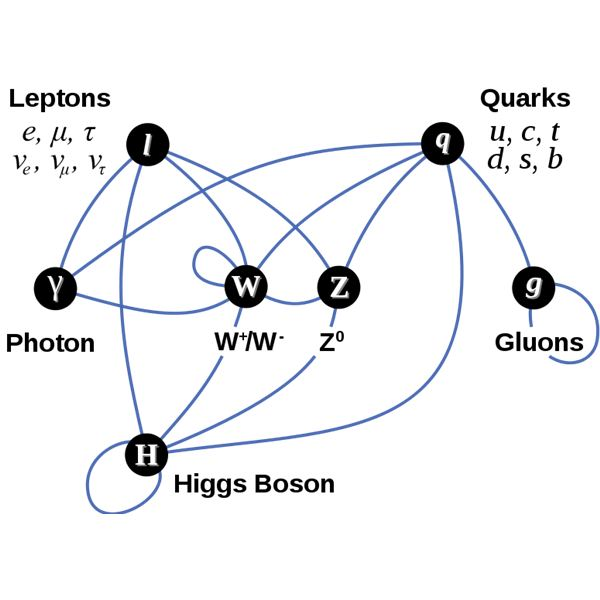
\includegraphics[width = 10cm]{Pictures/SM/elementaryParticles.jpg}
    %\missingfigure{Particles and boson}
    \caption{Summary of the Standard Model particles with their interactions.\\ \url{http://www.brighthub.com/science/space/articles/84750.aspx}}
    \label{fig:partInterac}
    \end{figure}   
    %\lettrine{\textgoth{T}}{he} 
    
    The \acrfull{SM} is a theory that describes the elementary structure of the matter surrounding us. 
    It is one of the most successful achievements in modern physics.
    The elegant theoretical framework of the \gls{SM} is able to provide good explanations of experimental results but is also able to predict a wide variety of phenomena.

    The \gls{SM} depicts the interactions between the fundamental constituents of matter, called particles.
    From a quantum point of view, a particle is defined by its intrinsic angular momentum, called spin. 
    This quantum number is a key to distinguish between the particles of 'matter' and the 'carrier force' particles.
    
    The half integers spin particles are obeying to the Fermi-Dirac statistics and are submitted to the Pauli exclusion principle:
    they can not occupy the same quantum state at the same time.
    These particles are called fermions.
    They are the constituents of the matter and are to the number of twelve.

    The fermions are divided into two categories: the leptons and the quarks. 
    The leptons are to the number of six: three charged particles and three neutral particles called neutrino.
    The first fundamental particle discovered in particle physics was the electron (e$^-$) at the end of the $19^{th}$ century.
    The two other charged leptons were discovered in 1937 for the muon ($\mu$) and in 1975 for the tau ($\tau$).
    Three neutrinos are associated to the three flavored leptons: the electron neutrino ($\nu_e$) discovered in 1953, the muon neutrino ($\nu_{\mu}$) in 1962 and the tau neutrino ($\nu_{\tau}$) discovered in 2000.

    The quarks are to the number of six.
    They can't be found alone in nature.
    They are carrying a quantum number: the color.
    The color quantum numbers are green, blue and red (and the anti-color associated).
    They are always in a bounded state to form composite particles that are colorless and are called hadrons.
    A quark and an anti-quark form an integer spin composite particle, a meson.
    Three quarks bounded together are called baryons. The most known baryons are the proton and the neutron.
    They are made of the up quarks (u) and the down quarks (d).
    The other quarks were discovered in the second half of the 20$^{th}$ century.
    The strange quark (s) was discovered in 1968, followed by the charm quark (c) in 1974.
    Then, the bottom quark or beauty quark (b) was discovered in 1977.
    The last quark discovered was the top quark (t) in 1995.  

    The fermions are also divided into three categories which depend on the mass of the particle.
    They are called generations.
    The first generation of particles is composed of the electron, the electron neutrino, the u and d quarks. 
    They form the ordinary matter.
    The two other generations are particles found in cosmic rays or in  collisions with accelerators.
    All the fermions and their properties are summarised in the table \ref{tab:fermions}.

    \begin{table}[!h]
      \begin{center}
        \begin{tabular}{c c c c c c c}
        \hline %----------------------------
        Type & Family & Particle  & L & B & Q$_e$ & Mass (MeV)  \tabularnewline
        \hline %----------------------------
        \hline %----------------------------
        \multirow{6}*{Leptons} & \multirow{2}*{1$^{st}$}    & $e$       & 1 & 0 & -1    & 0.511 \tabularnewline
                               & & $\nu_e$   & 1 & 0 & 0     & $< 2 \times 10^{-6}$ \tabularnewline
                               & \multirow{2}*{2$^{nd}$}    & $\mu$     & 1 & 0 & -1    & 105.66 \tabularnewline
                               & & $\nu_{\mu}$ & 1 & 0 & 0   & $< 2 \times 10^{-6}$ \tabularnewline
                               & \multirow{2}*{3$^{rd}$}    & $\tau$   & 1 & 0 & -1     & $1.78 \times 10^{3}$ \tabularnewline
                               & & $\nu_{\tau}$ & 1 & 0 & 0  & $< 2 \times 10^{-6}$ \tabularnewline
        \hline %----------------------------
        \hline %----------------------------
        \multirow{6}*{Quarks} & \multirow{2}*{1$^{st}$} & u & 0 & 1 & 2/3 & $2.3^{+0.7}_{-0.5}$\tabularnewline
                              & & d & 0 & 1 & -1/3 & $4.8^{+0.5}_{-0.3}$\tabularnewline
                              & \multirow{2}*{2$^{nd}$} & s & 0 & 1 & -1/3 & $ 95\pm 5 $ \tabularnewline
                              & & c & 0 & 1 &  2/3 & $1.275 \times 10^{3} \pm 2.5$ \tabularnewline
                              &\multirow{2}*{3$^{rd}$} & b & 0 & 1 & -1/3 & $4.66 \times 10^{3} \pm 30 $ \tabularnewline
                              & & t & 0 & 1 & 2/3 & $ 173.21 \times 10^{3} \pm 511 \pm 711$\tabularnewline
        \hline %----------------------------        
        \end{tabular}
      \end{center}
        \caption{Summary of the 12 fermions. L is a quantum number associated to the leptons. Its value is 1 for leptons and -1 for anti-leptons. B is a quantum number associated to the baryons. It is equal to 1 for a baryon and to -1 for an anti-baryon. \cite{Agashe:2014kda} }
        \label{tab:fermions}
    \end{table}
    

    The second kind of particles are integer spins particles and are labelled bosons or gauge bosons.
    They are following the Bose-Einstein statistics. 
    It means that the bosons are not limited to a single occupancy of the same state as the fermions.
    The bosons are the mediators of the four fundamental interactions.    

    \todo{Conservation laws and invariance}
    The particle physics is based on the conservation laws as well as the invariance.
    The invariance means that the physics is the same on every point of the Universe.
    For example, the speed of light is always $\sim 3.0 \text{ m.s}^{-1}$.
    
    The \gls{EM} is mediated by the photon $\gamma$, a massless and chargeless particle of spin 1.
    The EM is responsible for the interaction between two charged particles.
    The weak interaction which is responsible for the $\beta$ radioactive decay (a nucleon is able to transform into an other one with the emission of a lepton and a neutrino).
    The gauge bosons associated with the weak interaction are the neutral electrical charged boson $Z^0$, and two electrical charged one $W^+$ and $W^-$.
    The strong interaction is mediated by eight gauge bosons, the gluons.
    It is responsible for the nucleus and the hadrons cohesion.
    The last force is the gravitational interaction but it is not included into the \gls{SM}.
    Trying to find a framework where the equation of the general relativity used to describe the macro world and the equation of the quantum mechanics describing the micro world is a difficult challenge.
    From a quantum theory, the boson associated with the gravitational force might be the graviton, a spin 2 particle. 

    The Higgs boson (H) is a particle predicted by the S.M and has been discovered in 2012 at the Large Hadron Collider (LHC)
    It is the gauge boson of the Higgs mechanism.
    This mechanism is the mass generator of particles and will be presented later in section \ref{sec:higgsMechanism}.
    %assumed to be responsible for the generation of the masses and can be explained by the electroweak symmetry breaking.
    
    The table \ref{tab:bosons} summarises the different bosons of the \gls{SM}.

  \begin{table}[!h]
    \begin{center}
        \begin{tabular}{c c c c c}
        \hline %----------------------------
        Force & Gauge bosons & Mass (GeV/$c^2$) & Electric charge & Range \tabularnewline
        \hline %----------------------------
        \hline %----------------------------
        Electromagnetic & $\gamma$ & 0 & 0 & $\infty$\tabularnewline  
        \multirow{2}*{Weak} & $Z^0$ & 91.1876 $\pm$ 0.0021& 0 & \multirow{2}*{$10^{-18}$ m} \tabularnewline
             & $W^{\pm}$ & 80.3980 $\pm$ 0.0250 & $\pm 1$  &\tabularnewline 
        Strong & g (8 gluons) & 0 & 0 & $10^{-15}$ m \tabularnewline
        \hline %----------------------------
        \hline %----------------------------
            & H & 125 GeV & 0 & \tabularnewline
        \hline %----------------------------
        \end{tabular}
    \end{center}
    \caption{Summary of the interactions and the boson defined by the Standard Model. \cite{Agashe:2014kda} \\ N.B.: the graviton was not included in this table because the gravitational force is not taken into account in the SM. }
    \label{tab:bosons}
  \end{table}

      
    \subsection{Quantum Field Theory}

    The mathematical basis of the \gls{SM} is the Quantum Field Theory (QFT). All the interactions are described by the gauge group: 
    
      \begin{equation}
        SU_C(3) \otimes SU_L(2) \otimes U_Y(1)
      \end{equation}
    
    The gauge theory is invariant under a continuous set of local transformation.
    Taking the gauge symmetries and the least action into account, physicists were able to set up equations that describe the dynamic of the interactions by Lagrangian.
    The steps to build Lagrangian for the three forces and the unification of the EM and weak interactions are going to be presented. 
    
      \subsubsection{Quantum Electrodynamic}

     The Quantum Electrodynamic (QED) is the QFT that combines the electromagnetism formalism and the quantum mechanics formalism to describe the interaction thanks to a relativistic Lagrangian.
     As the charge $Q_e$ of the electron is invariant on every part of the Universe, the QED Lagrangian should be invariant under some transformations.
     The $U(1)$ gauge group is a unitary group of one dimension which is invariant under space transformations.

      Lets first consider the Dirac Lagrangian for a free fermion:
      
      \begin{equation}
        \mathcal{L}_{Dirac} = \overline{\Psi}\left(x\right) \left(i \gamma^{\mu}\partial_{\mu} - m \right) \Psi\left(x\right)
        \label{eq:diracLag}
      \end{equation}

      The Lagrangian is invariant under global U(1) transformation:

      \begin{equation}
            \begin{array}{rrccr}
             \Psi \left(x \right) & \rightarrow & \Psi^{'} \left(x \right)  & = & e^{-i\alpha} \Psi\left(x\right) \\
             \overline{\Psi}\left(x\right) & \rightarrow & \overline{\Psi}^{'}\left(x\right) & = & e^{i\alpha}  \overline{\Psi}\left(x\right) \\
            \end{array}
      \end{equation}

      The corresponding local symmetry is:

      \begin{equation}
            \begin{array}{rcccr}
             \Psi\left(x\right) & \rightarrow & \Psi^{'} \left(x \right) & = & e^{-i\alpha(x)} \Psi\left(x\right) \\
             \overline{\Psi}\left(x\right) & \rightarrow & \overline{\Psi}^{'}\left(x\right) & = & e^{i\alpha(x)}  \overline{\Psi}\left(x\right) \\
            \end{array}
      \end{equation}

      Although the mass term of the Lagrangian in the equation \ref{eq:diracLag} stays invariant under the local symmetry, the term containing a partial derivative is not anymore.
      A gauge field $A_{\mu}$ has to be added to the derivative to keep it invariant under local gauge transformation.
      %"To keep the derivative invariant under local gauge transformation, a gauge field $A_{\mu}$ has to be added to the derivative.
      The covariant derivative will be then: 

      \begin{equation}
        D_{\mu} \Psi\left(x\right) =  \left(\partial_{\mu} - i Q_e A_{\mu}\right) \Psi\left(x\right)
      \end{equation}

     The gauge field is not yet a dynamic field. To get a physical gauge field, a kinetic term should be added to the equation.
     This gauge invariant term that includes derivative from the $A_{\mu}$ field is:
    
     \begin{equation}
       F_{\mu \nu} \ = \ \partial_\mu A_\nu - \partial_\nu A_\mu
     \end{equation}

     The Lagrangian, which is local invariant, is the one that describes the QED:

    \begin{equation}
        \mathcal{L}_{QED} =  \overline{\Psi}\left(x\right)\left( i \gamma^\mu D_\mu - m \right) \Psi\left(x\right) - \frac{1}{4}F_{\mu \nu}\left(x\right) F^{\mu \nu}\left(x\right)
    \end{equation}

    A mass term $m A_{\mu} A^{\mu}$ for the field $A_{\mu}$ is missing because it is not gauge invariant. 
    That consideration matches to the fact that the photon is a massless boson.

    \todo{Add details on the QED: coupling...}

    \subsubsection{Weak interaction}

    In 1930, Pauli assumed that the continuous energy spectrum of the electron in the $\beta$ decay could be explained by the existence of a new particle to respect the principle of energy conservation. 
    It is a light particle, which does not interact so much with matter.

    After the discovery of the neutron by Chadwick in 1932, Fermi wrote a theory on weak interaction to explain the $\beta$ decay. \cite{Fermi:1934hr} 
    He postulated that the neutron is decaying into a proton by emitting an electron and a light neutral particle, called neutrino.
    In analogy to the electromagnetism, he proposed a current-current Lagrangian to describe the $\beta$ decay.
    \begin{equation}
\mathcal{L}_{weak} = \frac{G_F}{\sqrt{2}}\left(\overline{p} \gamma_{\mu} n \right) \left(\overline{e} \gamma_{\mu} \nu \right)
    \end{equation}

    where the $G_F$ is the Fermi constant $G_F = 1.166 \dot 10^{-5} GeV^{-2}$. 
    
    Nevertheless, the non-relativistic limit leads to an incomplete theory.
    The interaction considered with a 2-components spinor transforms a proton into a neutron without changing the position, the spin or the parity.
    However, T.D. Lee and C.N. Yang have postulated in 1956 that the weak interactions violate the parity after analysing the decays of the $\tau$ and $\theta$ particles\cite{1956PhRv..104..254L}.
    The Wu experiment \cite{1957PhRv..105.1413W} confirmed this hypothesis in 1957 by studying the decay of $^{60}$Co.

    The Fermi interaction was modified by Feynman and Gell-Mann\cite{PhysRev.109.193} to a $V \ - \ A$ theory\footnote{$V$ stands for vector and $A$ for axial-vector}.
    The vector current is now subtracted by an axial vector current. For example, the neutrino current is replaced by:

    \begin{equation}
        \begin{array}{rcc}
        \overline{e}(x) \gamma_{\mu} \nu & \rightarrow & \overline{e}\gamma_{\mu}(1 - \gamma_5 ) \nu \\
            & & = \overline{e} \gamma_{\mu} \nu - \overline{e}\gamma_{\mu} \gamma_5 \nu \\
        \end{array}
    \end{equation}

    It was established that the weak current has the form $V \ - \ A$ instead of $V \ + \ A$.
    The weak interaction is only coupling left-handed particles and right-handed anti-particles.
    
    The lagrangian describing the weak interactions can be written as a currents interaction:

    \begin{equation}
      \mathcal{L}_{weak} = - \frac{G_F}{\sqrt{2}} J^{\mu}J_{\mu}^{\dagger}
    \end{equation}
    
     and $J^{\mu}$ is a combination of leptonic and hadronic currents.

    Contrary to the QED, the weak interaction obeys to a non-Abelian symmetry group\footnote{A group is non-Abelian when the elements of the group are not commutating.}, the SU(2) symmetry group.
    The matter field could be represented as a doublet $\Psi_L$ and a singlet $\Psi_R$ of this group.

    \begin{equation}
      \begin{array}{cc}
        \Psi_L = 
         \begin{pmatrix}
           \nu_{eL} \\
           e_L
         \end{pmatrix}, & \Psi_R = e_R
      \end{array}
    \end{equation}

    The generators of the group are the three Pauli matrices $\sigma_i$, associated with a gauge field $W_{\mu}^i$.
    The bosons of the weak interactions are the $W^{\pm}$ and $Z$.

    As the left-handed leptons are combined into a doublet, a quantum number called weak isospin ($I_3$) is associated with them.
    The charged leptons have a weak isospin $I_3 = \frac{-1}{2}$ and for the neutrinos $I_3 = \frac{1}{2}$.
    Concerning the gauge bosons $W^{\pm}$ and $Z$, the weak isospin is respectively $I_3 = \pm 1, 0$.
    
    \subsubsection{Quantum Chromodynamics}
    
    The \gls{QCD} is the quantum field theory of the strong interaction.
    In this model, the interaction is due to an $SU(3)$ gauge group. 
    It produces 8 gauge fields called gluons.
    The spinors of this theory are the six quarks that form a triplet with respect to the gauge symmetry.

    The SU(3) gauge group is a group of $9 - 1 = 8$ real parameters and of 8 generators. 
    Those generators are the Gell-Mann matrices. 
    The normalised generators are defined by: 
    
    \begin{equation}
        T^a = \frac{1}{2}\lambda^a
    \end{equation}

    The structure constant $f^{abc}$ can be expressed as:

    \begin{equation}
        if^{abc} = 2 Tr([T^a,T^b]T^c)
    \end{equation}
     
    Some theories arguments and the results of experiments in high energy physics have required introducing six spinor fields, the quarks.
    Each of them is considered as a triplet state with respect to the SU(3) group:

    \begin{equation}
      q_i = 
        \begin{pmatrix}
          q_i^1 \\
          q_i^2 \\
          q_i^3 \\
        \end{pmatrix}
     \end{equation}
    
    where $q_i$ are the six quarks.
    These quarks can appear in three different states, called color and that are named red, blue and green.

    The local gauge symmetry U(1) should be included into the SU(3) group.
    
    The gauge field $A_{\mu}$ can be introduced in the group:
    
    \begin{equation}
      A_{\mu} = g_S A^a_{\mu}\frac{\lambda^a}{2}
    \end{equation}
     
    with a = 1,...,8 and corresponds to the 8 gluons.
    A mass term  $m_g A^{\mu}_a A^a_{\mu}$ would not be gauge invariant, it implies that the gluons have to be massless.

    The covariant derivative is then:

    \begin{equation}
      \begin{array}{rcl}
        D_{\mu} & = & \partial_{\mu} - i A_{\mu} \\
                & = & \partial_{\mu} - i g_S A^a_{\mu} \frac{\lambda^a}{2}
      \end{array}
    \end{equation}

    The QED field $F_{\mu \nu}$ is not gauge invariant in QCD.
    Nevertheless, an additional term to obtain gauge invariant field tensor can be introduced:
    
    \begin{equation}
      G^a_{\mu \nu} = \left( \partial_{\mu} A^a_{\nu} - \partial_{\nu} A^a_{\mu} \right) + g_S f^{abc} A^b_{\mu} A^c_{\nu}
    \end{equation} 

    Finally, the QCD Lagrangian is given by:

    \begin{equation}
      \mathcal{L} = \sum_{i=1}^6  \bar{q_i} \left(i \gamma^{\mu}D_{\mu} -m_i \right)q_i - \frac{1}{4} G_{\mu \nu}^{a} G_{a}^{\mu \nu}
    \end{equation}
    

    \section{The Glashow-Weinberg-Salam model}
    \todo{Rephrase the section title}

    Late 1960, a model of unification was postulated by Glashow, Weinberg, and Salam to describe the electroweak interaction (EW).
    The theory rests on a  $SU(2)_L \otimes U(1)_Y$ symmetry group.
    It is the simplest group which conserves the properties of EM charge conversion and parity violation of weak interaction.

    For the EW unification, the $U(1)_{EM}$ symmetry group describing the EM has to be rewritten.
    As the fermions are considered by left-handed doublets and right-handed singlets, the $U(1)_{EM}$ will break the gauge invariance.
    The weak isospin group $SU(2)_L$ is combined with the EM charge to create the hypercharge give by the Gell-Mann-Nishijima relation: 
  
    \begin{equation}
      Q = I_3 + \frac{1}{2}Y
    \end{equation}
   
    The $I_3$ term is the third component of the weak isospin.
    With the introduction of the hypercharge, the EM gauge invariance is conserved.

    The EW Lagrangian could be given as:

    \begin{equation}
      \mathcal{L}_{EW} = \mathcal{L}_{YM} + \mathcal{L}_{fermions} %+ \mathcal{L}_{H}
      \ref{eq:ewLag}
    \end{equation}

    The first term $\mathcal{L}_{YM}$ is the Yang-Mills Lagrangian that describes the bosons gauges interactions (kinetic term + interaction between bosons). 
    It has the form below:

    \begin{equation}
      \mathcal{L}_{YM} = - \frac{1}{4}\textbf{W}^a_{\mu\nu} \textbf{W}^{a\mu\nu} - \frac{1}{4}\textbf{B}_{\mu\nu}\textbf{B}^{\mu\nu}
    \end{equation}

    With 
    \begin{equation}
        \textbf{W}_{\mu\nu}  =  \partial_{\mu}\textbf{W}_{\nu} - \partial_{\nu}\textbf{W}_{\mu} - i g [\textbf{W}_{\mu},\textbf{W}_{\nu}]
      \label{eq:Wmunu}
    \end{equation}

    \begin{equation}
        \textbf{B}_{\mu\nu}  =  \partial_{\mu}\textbf{B}_{\nu} - \partial_{\nu}\textbf{B}_{\mu}
        \label{eq:Bmu}
    \end{equation}
    
    In the equation \ref{eq:Wmunu}, $\textbf{W}_{\mu} = \sum W^i_{\mu}\sigma^i/2$ is a vector of three gauge fields associated to $SU(2)_L$ and $\sigma^i$ are the Pauli matrices. 
    The term $[\textbf{W}_{\mu},\textbf{W}_{\nu}]$ is associated to the interactions between the gauge fields.
    In the equation \ref{eq:Bmu}, $\textbf{B}_{\mu}$ is the only gauge field associated to the $U(1)_Y$.

    The Lagrangian describing the fermions field is given by:

    \begin{equation}
      \mathcal{L}_{fermions} = \overline{\Psi}_L\gamma^{\mu}D_{\mu}\Psi_L + \overline{\Psi}_R\gamma^{\mu}D_{\mu}\Psi_R
    \end{equation}
      
    \begin{equation}
      \text{With} \ D_{\mu}\Psi_L = \left( \partial_{\mu} + ig \textbf{W}_{\mu} - i \frac{g'}{2}Y\textbf{B}_{\mu}\right)\Psi_L \text{ and } D_{\mu}\Psi_R = \left(\partial_{\mu} - i\frac{g'}{2}Y\textbf{B}_{\mu}\right)\Psi_R
      \label{eq:derivativeEW}
    \end{equation}
    
    In the equation \ref{eq:derivativeEW}, the covariant derivative has two forms. 
    The weak interaction does not allow coupling of the W bosons to right-handed fermions whereas the $\gamma$ and Z bosons do.

    With the EW Lagrangian described above, the gauge bosons were considered as massless fields.
    The electroweak interaction does not allow a $m\overline{\Psi}\Psi$ term because it does not transform as a scalar under $SU(2)_L \otimes U(1)_Y$.
    Moreover, the $m^2 \textbf{W}_{\mu} \textbf{W}^{\mu}$ violates the $SU(2)_L$ gauge invariance of the Lagrangian.
    The mass terms associated with the physical fields of the gauge bosons are given by spontaneous symmetry breaking via the Higgs mechanism.


%    The Standard Model constitutes one of the most successful achievements in modern physics.
%    One of its strength is to provide an elegant theoretical framework to describe the known experimental facts about particles, but also it was able to predict 
%    the existence of a mechanism to generate the particle masses via the Higgs mechanism.


     \subsection{Symmetry Breaking mechanism and Goldston theorem}
    
    Before to introduce the Higgs mechanism, we will study the spontaneous symmetry breaking for a global symmetry.
    This phenomenon is also seen in phase transitions or laser theory.

    Let's consider first the Lagrangian density for a complex scalar field $\phi$:

    \begin{equation}
      \mathcal{L} = \partial^{\mu}\phi^{*} \partial_{\mu}\phi - \mu^2\phi^{*}\phi - \lambda (\phi^{*}\phi)^2
      \label{eq:ssbLagrangian}
    \end{equation}

    The first component of the Lagrangian density corresponds to the kinetic term of a complex scalar field, while the second component is related to a scalar potential.
    The coefficient $\mu^2$ is a real parameter. Nevertheless, depending on its sign, the potential can take two forms.

    If $\mu^{2} > 0$, the symmetry is unbroken and the potential has a minimum at $\phi = 0$ which does not degenerate.
    It describes a particle with a mass $\mu$ and a quartic self-coupling.
    As the transformation $\phi \rightarrow  - \phi$ is respected, this solution is a symmetric one.

    When $\mu^{2} < 0$, there is not a unique ground state for this system but multiple states with the same vacuum energy.
    The minima is located on a circle of radius:

    \begin{equation}
      v = \sqrt{\frac{- \mu^2}{2\lambda}} > 0
      \label{eq:v}
    \end{equation}

    By choosing a particular solution as the ground state, the symmetry gets spontaneously broken.

    A parametrisation of the excitations around the ground state is possible by introducing a new field $\phi$:

    \begin{equation}
      \phi(x) = \frac{1}{\sqrt{2}} \left( v + \rho(x) + i\Theta(x) \right)
    \end{equation}

    The value $v$ is given by one of the solution from equation \ref{eq:v}, $\rho(x)$ and $\Theta(x)$ are real fields.

    By adding the new field in the equation \ref{eq:ssbLagrangian}, the Lagrangian becomes:

    \begin{equation}
      \mathcal{L} = \frac{1}{2} (\partial_{\mu}\rho)^2 + \frac{1}{2}(\partial_{\mu}\Theta)^2 - \lambda v^2 \rho^2 - \lambda v (\rho^3 +\rho \Theta^2) - \frac{\lambda}{4}(\rho^2 + \Theta^2)^2
    \end{equation}

    The field $\rho(x)$ describes a state of mass $m_{\rho} = 2 \mu^2$, coupled to the massless field $\Theta(x)$.

    The field $\Theta(x)$ describes excitations around a direction in the potential.
    The excitations are not costing any energy, so they correspond to massless bosons called Goldstone bosons.


    \subsection{Higgs mechanism}
    \label{sec:higgsMechanism}

    As we have seen with the Lagrangian of the QED and QCD, the bosons generated are massless. Nevertheless, the W$^{\pm}$ and the Z bosons have a mass and the equation \ref{eq:ewLag} of the EW interaction does not include a mass generator. 
    The origin of the fermions masses is solved in the \gls{SM} thanks to the Higgs-Englert-Brout mechanism \cite{PhysRevLett.13.508}\cite{1964PhRvL..13..321E}.

    Lets consider first a doublet of complex scalar fields $\Phi$:
    
    \begin{equation}
       \Phi = \begin{pmatrix}
                \phi^{+}\\
                \phi^{0}
              \end{pmatrix}
    \end{equation}

     The invariant Lagrangian density under $SU(2)_L \otimes U(1)_Y$ gauge transformation is:

    \begin{equation}
      \mathcal{L} = \left(D^{\mu} \phi \right)^{\dagger} \left( D_{\mu} \phi \right) - V(\phi)
      \label{eq:lagrangianHiggs}
    \end{equation}    
    
    The covariant derivative is the one of $SU(2)_L \otimes U(1)_Y$ given by the equation \ref{eq:derivativeEW} and represents the kinetic term.
    %The Higgs potential $V(\phi)$ is: $V(\phi) = \mu^2 \phi^{\dagger}\phi + \lambda(\phi^{\dagger}\phi)^2$.
    The Higgs potential is similar to the one considered first and has also two solutions depending on the sign of $\mu^2$.
    Let's focus only on the negative solution. 
    There is an infinite set of degenerated states with minimum energy:

    \begin{equation}
      \phi_0 = \sqrt{\frac{1}{2}}
      \begin{pmatrix}
        0 \\
        v
      \end{pmatrix}
      \text{ with } \ v = \sqrt{\frac{- \mu^2}{\lambda}} > 0
      \label{eq:v}
    \end{equation}

    Let's expand the field $\Phi$ around its minima by including a field $h(x)$ which describes quantum fluctuations and three massless Goldstone fields, denoted $\theta^i(x)$:

    \begin{equation}
      \Phi(x) = e^{i\frac{\sigma_i}{2}\theta^i(x)} \frac{1}{\sqrt{2}}
                \begin{pmatrix}
                   0 \\
                   v + h(x)
                 \end{pmatrix}
      \label{eq:fieldHiggs}
    \end{equation}

     
    %The substitution of \ref{eq:fieldHiggs} into \ref{eq:lagrangianHiggs}, 

%    The first term corresponds to the kinetic term of a scalar field.
%    The second term is a scalar potential that is invariant under $SU(2)_L$ and it is:
%
%    \begin{equation}
%      \begin{array}{lr}
%        V(\phi) = \mu^{2}\phi^{\dagger}\phi + \lambda \left(\phi^{\dagger}\phi\right)^2  & , with \ \lambda > 0 \\
%      \end{array}   
%    \end{equation}
    
    A particular gauge can be defined in a way that the Goldstone fields are absorbed by the physical field of $SU(2)_L \otimes U(1)_Y$.
    It implies the apparition of mass terms in equation \ref{eq:lagrangianHiggs}.
    First, we are interesting in the mass generation mechanism, we will focus only on the impact of the new field on the derivative covariant, we will omit any h-mixed terms and drop down the partial derivative:

    \begin{equation}
      \left|\left(i\frac{g}{2}\textbf{W}_{\mu} +i\frac{g'}{2}Y\textbf{B}_{\mu}\right) \Phi \right|^2 = \frac{1}{8}\left|
              \begin{pmatrix}
                 gW^3_{\mu} +g'B_{\mu} & g(W^1_{\mu} - i W^2_{\mu}) \\
                 g(W^1_{\mu} + i W^2_{\mu}) & - g W^3_{\mu} + g'B_{\mu}
              \end{pmatrix}
              \begin{pmatrix}
                0 \\
                v
              \end{pmatrix}
         \right|^2
      \label{eq:derHiggs}
    \end{equation}

    The charged fields can be expressed as a linear combination of gauge field:

    \begin{equation}
      W^{\pm}_{\mu} = \frac{W^1_{\mu} \mp iW^2_{\mu}}{\sqrt{2}}
    \end{equation}

    The eigenstates are rewritten as decorrelated terms representing the neutral fields from the EW symmetry group:

    \begin{equation}
      Z_{\mu} = \cos{\theta_{w}W^3_{\mu}} - \sin{\theta_{w}B_{\mu}}
    \end{equation}
    \begin{equation}
      A_{\mu} = \sin{\theta_{w}W^3_{\mu}} + \cos{\theta_{w}B_{\mu}}
    \end{equation}

   $\theta_{w}$ is the Weinberg angle and represent a bound between the coupling $g$ and $g'$:
   
   \begin{equation}
   \sin{\theta_{w}} = \frac{g'}{\sqrt{g^2+g'^2}} \ and \ \cos{\theta_{w}} = \frac{g}{\sqrt{g^2+g'^2}}
   \end{equation} 

    The equation \ref{eq:derHiggs} becomes:

    \begin{equation}
      \begin{array}{rcl}
     \left|\left(i\frac{g}{2}\textbf{W}_{\mu} +i\frac{g'}{2}Y\textbf{B}_{\mu}\right) \Phi \right|^2 & = & \frac{1}{8} \left| 
        \begin{pmatrix}
          A_{\mu}\sqrt{g^2 + g'^2} & gW^-_{\mu} \\
          gW^+_{\mu} & -Z_{\mu}\sqrt{g^2 + g'^2}
        \end{pmatrix}
     \right|^2 \\
      & = & \frac{1}{2}M^2_Z ZZ^* + \frac{1}{2}M^2_W W^-W^+
      \end{array}
    \end{equation}

    With $M_Z = \frac{1}{2}v\sqrt{g^2 + g'^2}$ and $M_W = \frac{1}{2} vg$, the mass of the Z boson and the W$^{\pm}$ bosons. 
    The mass of the photon is coherent to the expectation and is null. 

    The Higgs mechanism implies the existence of a massive gauge field, the Higgs boson.
    It is coupled to the other bosons and also to itself.
    This could be shown by extending the Higgs potential with the field defined in equation \ref{eq:fieldHiggs}:

    \begin{equation}
      -\lambda v^2h^2 - \lambda v h^3 - \frac{1}{4}\lambda h^4
    \end{equation}

    The first term gives the mass of the Higgs boson, $M^2_H = 2\lambda v^2$, while the second and third terms are the Higgs self-interactions.
    The Higgs mass can not be predicted by the theory because it is given by a function of the parameter $\lambda$, which is one of the free parameters of the \gls{SM}.
    
    \begin{figure}[h]
    \centering
      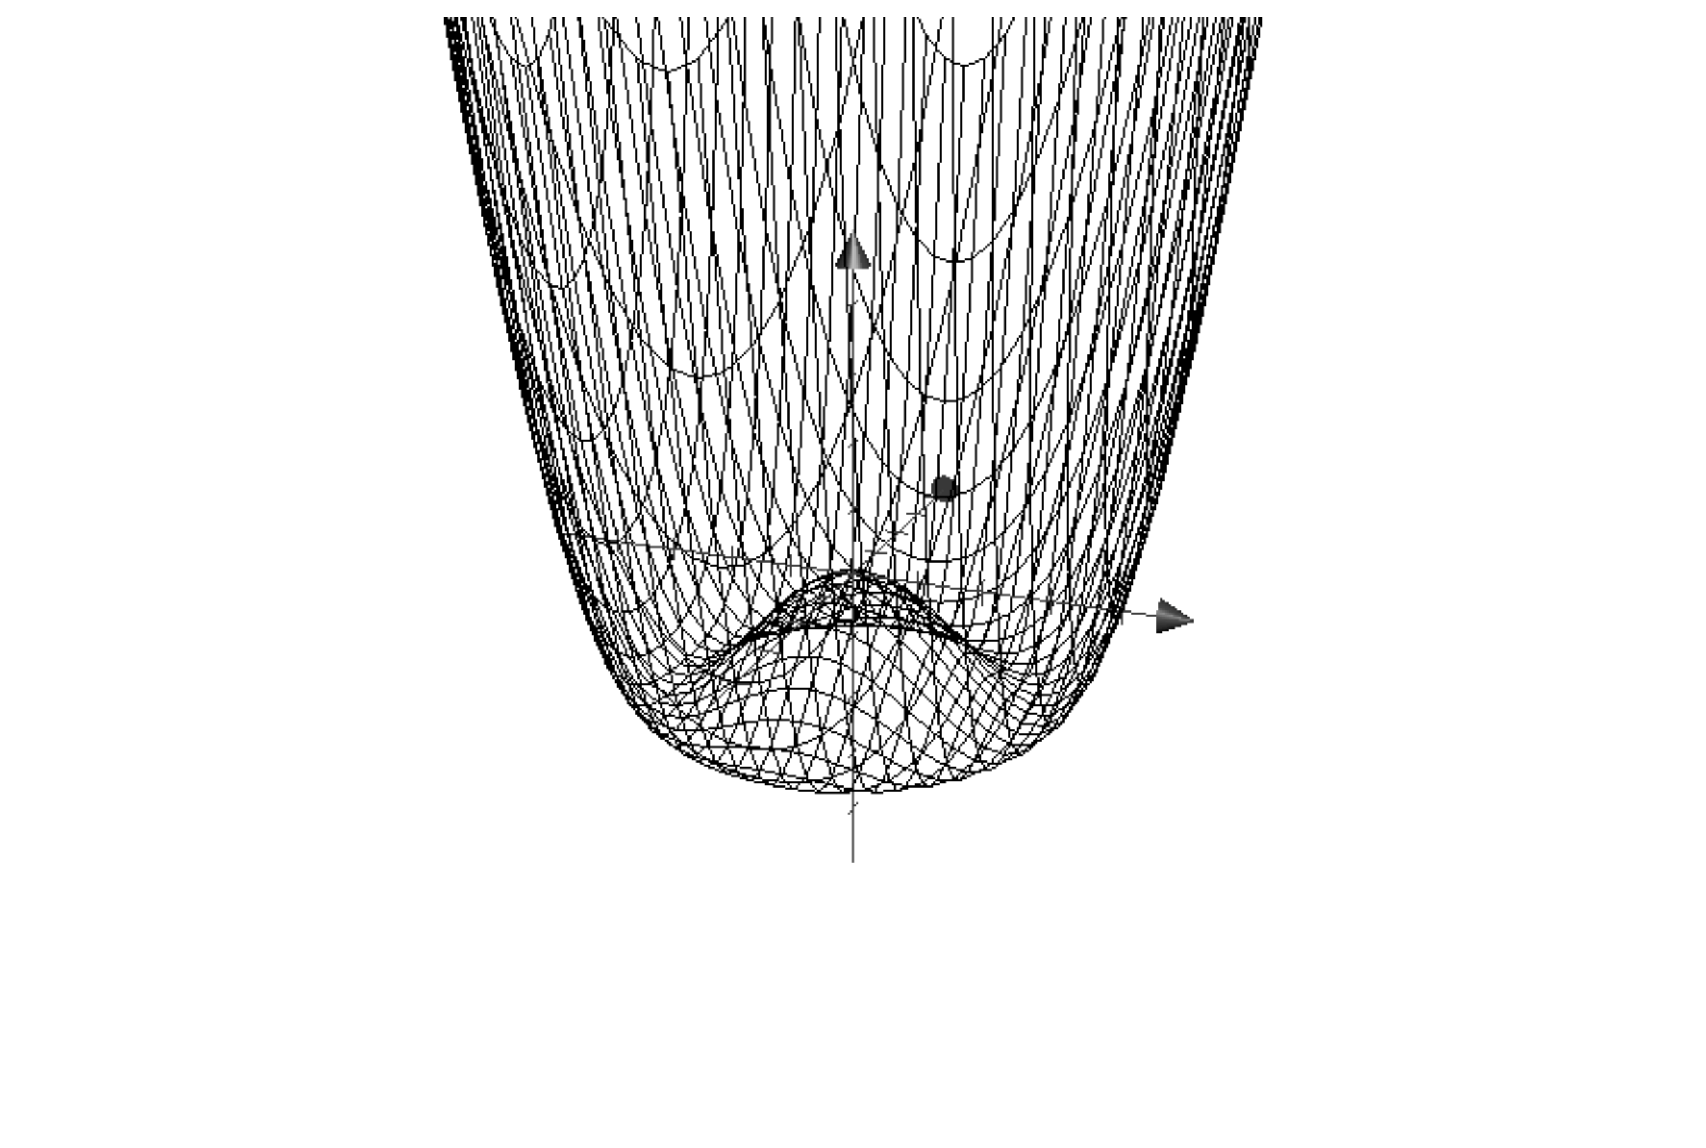
\includegraphics[width = 10cm]{Pictures/SM/mexHat.eps}
      %\missingfigure{Mexican hat}
    \caption{Scalar potential: ADD A GOOD CAPTION.}
    \label{fig:scalarPotential}
    \end{figure}

    \todo{Yukawa couplings with fermions}

  \section{Beyond the Standard Model}

%    The Standard Model constitutes one of the most successful achievements in modern physics.
%    One of its strength is to provide an elegant theoretical framework to describe the known experimental facts about particles, but also it was able to predict 
%    the existence of a mechanism to generate the particle masses via the Higgs mechanism.

  The \gls{SM} constitutes one of the most successful achievements in modern physics.
  One of its strength is to provide an elegant theoretical framework to describe the known experimental facts about particles, but also it was able to predict 
  the existence of a mechanism to generate the particle masses via the Higgs mechanism.
  Nevertheless, a lot of mysteries in the Universe are not explained by this theory. 
  
  \subsection{Limitations of the Standard Model}

  Despite the fact that the experimental results are not contradictory to the \gls{SM}, the theory is far away to be the answer to all the questions.
  The particle physics community is facing a challenge to find the ultimate theory of everything.
  An exhaustive list of some limitations is going to be presented.

    \subsubsection{Free parameters}

    Up to 19 free parameters are used in the \gls{SM} and this theory does not explain their existence.
    Even if it is not as major problem for the physics itself, the particles physics community has a lack of understanding and explaining these values.
    The free parameters are: 
    \begin{itemize}
      \item the masses of the nine fermions
      \item the coupling constants $g$ and $g'$ of the $U(1)$ and $SU(2)$ groups
      \item the coupling constant of the strong interaction $\alpha_s$
      \item the angles of the CKM matrix
      \item the Higgs boson mass and the $vev$ parameters that allows CP violation in \gls{QCD} Lagrangian. 
    \end{itemize}

    %The \gls{SM} does not explain the existence of the free parameters, which are to the number of 19.\todo{List of the 19 free-parameters: This parameters are the masses of the fermion (9 parameters), the coupling constants $g$ and $g'$ of the $U(1)$ and $SU(2)$ groups, the coupling constant of the strong interaction $\alpha_s$, the angles of the CKM matrix, the Higgs boson mass and the $vev$, parameters that allows CP violation in QCD Lagrangian
%}
    %It does not explain also why there are three generations of particles and why the gap between generations is spread over five orders of magnitude.

    %This is not really a problem for the physics itself, nevertheless, the particles physics community has a lack of understanding these values.
  
    \subsubsection{Hierarchy problem}

    The hierarchy problem refers to two main energy scales problem about the \gls{SM}.

    First of all, the difference between the energy scale of the \gls{SM} and the Planck scale is of the seventeen orders of magnitude.
    No "intermediate" physics have been found between the two scale.

    A second problem occurs while considering the Higgs boson mass.
    The \gls{SM} does not predict its mass, but it sets some theoretical bounds with respect to $\Lambda$, the scaled energy at which the \gls{SM} is not valid anymore.
    The theoretical Higgs boson mass is higher that what it should be compared to the EW scale.
    The Higgs boson interacts with the particles of the \gls{SM} (fermions, W and Z boson), but it also interacts with himself.
    Due to the scalar nature of the boson, they are quartic divergences while calculating the loop corrections.
    The quantum corrections, which take into account the coupling of the Higgs boson, are $\Lambda^2$ divergent and lead to a huge Higgs boson mass.
    To avoid that, delicate cancellations should occur between the quantum corrections.
    These cancellations are known as the fine-tuning problem. 
    
    \subsubsection{Gravitation}

    Although particles physicists are dreaming of a "theory of everything" that will unify the electroweak, strong and gravitational interactions,
    there is no viable theory to describe the gravity in a quantum point of view to include it in the \gls{SM} and which would be still valid at a macro-scale.

    \subsubsection{Neutrino mass}

    The neutrinos defined by the \gls{SM} are assumed to be exactly massless.
    Nevertheless at the end of the 90's, the Super Kamiokande experiment had surprising results\cite{Super-Kamiokande-Oscillation}.
    There was a lack on the expected solar and atmosphere neutrinos flux. 
    The result was interpreted by an oscillation of neutrinos between the three leptonic flavors.
    However, the oscillation is possible only if the neutrino has a mass.
    That phenomenon could be considered as a proof of physics beyond the \gls{SM}.

    \subsubsection{Matter-antimatter asymmetry}

    As discussed at the beginning of this chapter, the \gls{SM} defines an equal number of particles and anti-particles. 
    In the case of the Big Bang theory, it is assumed that the matter and antimatter were created in an exactly equal amount, a mechanism has favoured electrons, protons, and neutrons with respect to positrons antiprotons and antineutrons.
    If the amount of matter and antimatter was equal, our Universe would have been completely annihilated.
    The matter domination could be a local phenomenon with an antimatter surrounding the region. 
    However, the region of contact between matter and antimatter would be a violent place of interaction, which would disturb the cosmic microwave background.

    An assumption to explain the asymmetry is that the antimatter was produced in an infinity proportion compared to the matter.
    Hence, the annihilation as lead to create a Universe only made of matter.
    A mechanism which tends to prefer the matter has been observed in the study of the kaon oscillation.
    This particle is able to transform spontaneously to its own anti-particle and vice-versa.
    Nevertheless, this transformation is not symmetric: the kaon is slower to turn into an antikaon than the inverse transformation.
    Unfortunately, the \gls{SM} provides no explanation about that mechanism.
 
    \subsubsection{Dark Matter and dark energy}
    
   % \todo{Rephrase dark matter and dark energy}
    Several astrophysical observations are indicating that the Universe is made not only of visible matter but also of matter that seems to be invisible to the electromagnetic interaction, the dark matter.
    In 1933, a measurement of the galaxies velocities in the Coma cluster to determine the cluster mass gives a surprising result.
    The mass was more than two orders of magnitude bigger than the mass of visible stars in the cluster.
    It was found that the matter of the \gls{SM} describes only 5\% of the Universe content. 
    The rest of the Universe is made of 22\% of dark matter and around 73\% of dark energy.
    The neutrinos are possible candidates to dark matter, as it couples to \gls{SM} matter via only weak interaction, but they cannot account for the entire density of the universe.
    Nowadays only twelve particles (plus the anti-particles associated) have been observed. 
    The idea of dark matter comes from the way we the mass of a galaxy is estimated.

    \subsection{Theories beyond the Standard Model}

      \subsubsection{Supersymmetry}
    
      The Supersymmetry (SUSY) is a QFT, that relates the elementary fermions known to corresponding bosons, called sfermions and the bosons to corresponding fermions, sbosons \cite{Signer2009}.
      The related particles are called super-partners.
      They have the same mass, the same quantum numbers but the spin is differing by a half factor.
      SUSY is a broken symmetry. 
      This will allow the super-particles to acquire very high masses.

      SUSY is a good candidate for physics beyond the \gls{SM}. 
      It will solve the hierarchy problem without any fine tuning.
      For example, the loop contributions of one particle to the Higgs are cancelled by the loop contributions of its super-partner.
      It will be able to provide a framework for the unification of the three gauge interactions at a GUT scale.
      The lightest super-particle is a good candidate for the Dark Matter.

      Despite it will answer many questions from the \gls{SM}, there is a lack of understanding why SUSY is a broken symmetry.
      
      \subsubsection{Grand unification theory}
      
      After the success of the electroweak unification, the next step is to include the strong interaction to build the Grand Unification Theory (GUT), an extension of the \gls{SM}.
      In this framework, the three forces are different manifestations of a single interaction. 
      It includes the $SU(3)_C \otimes SU(2)_L \otimes U(1)_Y$ symmetry group into a larger $SU(5)$ group. 
      The quarks and leptons are ordered in left decuplets and right quintets.
      The coupling constants are described by only one parameter.  
      There are 24 mediators, the 12 mediators of the \gls{SM} plus 6 X mediators (charge $\pm4/3$ and 3 colors) and 6 Y mediators (charge $\pm1/3$ and 3 colors).
      It predicts the existence of new particles as leptoquarks\footnote{Coupling between a lepton and a quark}, multiple Higgs bosons and new currents.

      Unfortunately, the theory is not validated because of its prediction of the proton lifetime. 
      The first GUT was introduced by Georgi and Glashow in 1974 and was predicting a decay of the proton. 
      The actual experimental limit of the proton lifetime is set to $5 \times 10^{32}$ years, whereas the predicted lifetime defined by the SU(5) group is one order of magnitude lower.
      \cite{Agashe:2014kda}

      \subsubsection{Technicolor}

      The technicolor is a theory that explains the mass generation.
      Contrary to the EW symmetry, the masses of particles are not generated by the spontaneous symmetry breaking but they are generated by a strong gauge interaction.
      This interaction is strong and confined at the energy that has been experimentally probed.
      The approach of the theory avoids the hierarchy problem induced by the \gls{SM}.
      
      \subsubsection{String theory}

      The particle physicists have the dream of unifying the forces of the nature to have only one single interaction with four different manifestations.
      The string theory proposes a framework for the "theory of everything".
      The basic unit of matter is no more considered as particles but a one-dimensional string of which particles are various vibrational modes.

      The string theory is a theory of quantum gravity.
      It tries to unify the gravitation to the quantum 
      Extra dimensions of 10 -11 space-time dimensions.
      Possible explanation for the hierarchy problem.

    \section{Conclusions}

    We have seen the beauty and the limits of the \gls{SM}.
    The high energy physics community is trying to study as far as possible the limit of the \gls{SM} and is also trying to find some proof of new physics beyond the \gls{SM}.
    The (LHC) at CERN has permitted in 2012 to point out the existence of a Higgs boson.  
    Nevertheless, the beam structure of the LHC is not efficient enough to perform very precise measurements.
    Because of the collision between protons, the energy of the collision can't be exactly known.
    The next chapter deals with a future experiment in high energy physics, where electrons and positrons are used to probe the matter instead of protons and antiprotons.


	  
    \chapter[The ILC]{The future of high-energy physics: the International Linear Collider}
\label{chap:ILC}


 %Introduction on the limits of the LHC and why a new colliding experiment is needed
 % First part: describing the main characteristics of the ILC (energy scale, legnth, luminosity)
 %   -> Design (e+/e- sources, damping ring, main linacs, beam delivery system and interaction region )
 %   -> Beam properties
 %   -> Background: beam-beam interaction (luminosity enhancement ~2 BUT hard bremstrahlung that degrades the energy spectrum), pair background (coherent and incoherent production of e+e-)
 % Second part: Detector
 %   -> Option for two experiments (PUSH-PULL)
 %   -> Main differences between the ILD and the SiD
 %   -> Talking about the ILD (VTX, SIT, TPC, f)

  Since 2008, the Large Hadron Collider (LHC) is actually the most powerful tool in high energy physics to have a better understanding of the universe, particularly with the discovery in 2012 of a new particle compatible to the boson predicted by the spontaneous symmetry breaking of the SM \cite{Aad2012, Chatrchyan2012}.
  Although the LHC is an impressive machine able to reach the highest energy scales of collisions available on Earth with a centre-of-mass energy of 14 TeV, the complex environment of the events generated hides the access to some fundamental parameters. 
  To achieve more precise measurements of the Higgs boson, but also to test the validity of the SM and other physics theories introduce in the chapter \ref{chap:SM}, the high energy physics community has merged on the necessity to build a linear electron-positron collider, that will work as a complementary accelerator to the LHC.
  
  This chapter will explain the motivations to invest a huge amount of money in a new great world project. It will present the complementary nature of the lepton and hadron colliders and the main advantages of the lepton collisions will be discussed.
  After giving an overview of the ILC with its basic design and the experiment models, we will focus on the design of one of the experiments: the International Large Detector (ILD).

 \minitoc
  
  \section{The ILC machine}
 
  Before to introduce the ILC machine and explain the reasons to invest in such a project, I will give an overview of the LHC abilities and the limits of this giant machine.
  The most impressive accelerator ever built is located at CERN in Geneva, Switzerland. 
  It is the world's largest particle accelerator, with a circumference ring of nearly 27 kilometers, straddling the Swiss and French borders.
  It is designed to collide two counter rotating beams of protons or heavy ions, with a possibility to reach centre-of-mass energies of 14 TeV with a high peak luminosity of $10^{34} \text{ cm}^2 \text{s}^{-1}$.
  The goals of the LHC are to perform further tests on the SM, search for new forces or produce dark matter candidates. 
  Indeed, the collider covers a wide energy range at the constituent level while running at a fixed beam energy.
  Unfortunately, the measurements can not reach the highest precision.
  
  Complementary to a discovery machine such as the LHC, a machine to perform precise measurement should be built: the lepton collider.

    \subsection{Advantages of a linear lepton collider}
    
    First of all, during each collision at an hadron collider, only a part of the total centre-of-mass energy is available for the process evolved, so the initial four-vector momentum is not known. 
    By colliding leptons, which are structureless objects, the full centre-of-mass energy is available for the elementary process. 
    The initial four-vector momentum of an interaction is exactly known, hence the event can be fully reconstructed.

    Secondly, with a lepton collider, the beam energy is tunable and both electron and positron beams can be polarised. 
    The selection of an appropriate polarisation can boost the signal and suppress the background cross-section. 

    Thirdly, as seen on the first point, at the LHC, only a fraction of the partons are contributing to the interesting process. 
    The proton-proton interaction cross section is dominated by inelastic background QCD processes.
    The signal event is then accompanied by large backgrounds produced by the interaction of other partons collisions.
    This background has an impact on the detector design (high radiation tolerance and selective trigger implementation) and masks the elementary process of interests. 
    The lepton colliders do not suffer from this kind of background and at similar energies, the event rate is lower as those of hadron colliders.
    So, the detectors do not have to handle extreme data rates and they can be use without any trigger.
    This will allow to get a better sensitivity to any possible signature of new physics.

    % - Leptons are structureless -> Well known 4-vector momentum to reconstruct fully the event
    % - Quarks are made of partons => Impossible to know exactly the 4-vector momentum
    % - Partons that do not participate to the collisions contribute to parisitic soft interaction (QCD bg)
    %       => Hide elementary processes (small polar angle)
    %       => Needs implementation of trigger
    % - Beam energy tunable and polarisation of e+/e- can enhance the signal and suppress the background cross-section 
    
    % LINEAR VS CIRCULAR COLLIDER!
    \subsection{ }
  
  blablabla

  \begin{figure}
    \centering
    \missingfigure{Design of the ILC}
    \caption{Basic design of the International Linear Collider}
    \label{fig:ILC}
  \end{figure}

  \section{Design of the ILC}
    \subsection{Baseline design}
    \subsection{Beam parameters}
    \subsection{Background}

  \section{The ILC detectors concept}

    \subsection{Overview of the two experiments}
    
  Although the ILC is a linear collider with only one beam line, two experiments will participate.
  The duplication of the beam to get two permanent fixed detectors is too expensive and difficult to built.
  Instead, the collaboration has the idea to have only one interaction point.
  A push/pull system will allow to change the detector 

  Two detector designed with complementary features have been developed. 
  Their designs will reach the ILC precision measurements and search for new physics. 
  They are optimised for the particle flow algorithm (PFA) to measure the final states with high accuracy.
  This leads to a high hermeticity, high granular calorimeters and excellent tracking and vertexing. 
  The two experiments are the Silicon Detector (SiD) and the International Large Detector (ILD) and a global comparison of the two detectors is going to be presented on the next subsection.

      \subsection{SiD VS ILD}

    \subsection{I don't know th title name}
      \subsubsection{Vertex detector}
      \subsubsection{Tracking}
      \subsubsection{Calorimeters}


    \chapter{Physics at the ILC}
\label{chap:phyics}

  In chapter~\ref{chap:SM}, the framework of particles physics was described. 
  Since the beginning of the high-energy physics, different experiments have been performed to confirm the exactness of the \acrfull{SM} and search for new phenomena beyond the \gls{SM}.
  Depending on the type of colliders used, the measurements do not achieved the same precision. 
  For example, the \gls{LHC} with its high luminosity and high energy beam, is able to reach new energy scales, whereas the \gls{ILC} with its electron/positron interaction at lower energy beam is able to perform more precise measurements, due to the known initial state and the \gls{QCD} free background. 
  Along this chapter, the physics scenarios that are scheduled at the \gls{ILC} are discussed. 
  Afterward, the emphasis will be on the Higgs boson physics and the measurement planned at the \gls{ILC}. 
  The last section aims to introduce a physics analysis scenario to study the processes leading to a Higgs boson and two neutrinos in the final state.
 
 \minitoc

  \section{Potential studies}

  As seen in chapter \ref{chap:ILC}, the \gls{ILC} will have a vast and variable tunable centre-of-mass energy.
  Due to the features of an $e^-e^+$ collider, there is no contribution from strong interaction background and the initial state of collision is well defined, contrary to the \gls{LHC}.
  Moreover, the electroweak background is calculable and controlled.
  All the conditions are reunite to perform precise physics measurements and to look for an evidence of new physics beyond the \gls{SM}.
  The different measurements which will be performed are presented below.

  At the centre-of-mass energy of $\sqrt{s} = 250~\rm{GeV}$, studies on the Higgs boson couplings will be performed, as well as measurements on the quantum numbers associated to this boson.
  The main Higgs boson production process at this energy is via Higgs-strahlung.
  The measurements could be performed using the recoil mass method independently of the Higgs boson decay products.
 
  Then, for a centre-of-mass energy between 350 and 400 GeV, two studies are achievable. 
  The $WW$-fusion process starts to rise and permits to measure the couplings of the Higgs boson to the $W$ ones in order to look for deviation from the Standard Model. 
  Moreover, this channel allows to study some rare decays. 
  This energy range corresponds also to the threshold of the top quark pairs production.
  Due to the top quark life-time, the two quarks created are not in a bounded-state.
  By performing a threshold scan, the mass of the top quark can be measured with a precision reaching 100 $\rm{MeV/c}^2$.

  The nominal energy of the \gls{ILC} is achieved at $\sqrt{s} = 500~\rm{GeV}$.
  This energy scale is suitable to look for supersymmetry candidates and possible extended states of the Higgs boson.

  An upgrade of the ILC to reach the centre-of-mass energy $\sqrt{s} = 1~\rm{TeV}$ is also scheduled.
  Up to $1~\rm{TeV}$, new measurements are possible, such as the coupling of the Higgs boson to the top quark, the Higgs boson self-coupling, or its compositeness.
  Although, search for new exotic particles and physics beyond the \gls{SM} is possible.

  Another option possible for the \gls{ILC} is to perform more precise measurements on the $Z$ and $W$ bosons.
  At the centre-of-mass energy of $\sqrt{s} = 91~\rm{GeV}$, the program \textit{GigaZ} will be able to collect more $Z$ boson events than \gls{LEP} did.
  The luminosity of the \gls{ILC} will be two to three times higher than what was achieved in the past.
  At the $Z$ resonance, the data collect will allow studying the asymmetries of the $Z$ boson couplings.
  The \textit{MegaW} program will be performed at the centre-of-mass energy of $\sqrt{s} = 160~\rm{GeV}$ reaching the $WW$ production threshold and trying to measure the $W$ boson mass with a precision of $\rm{MeV/c}^2$.
  At higher energy, it will also be possible to measure more precisely the $W$ boson couplings.
 
  Table~\ref{tab:physicsAtIlc} summarises the different physics programs at the \gls{ILC} for the different energy reachable.  

  \begin{table}[h]
    \centering
    \begin{tabular}{c c c}
      \hline %----------------------------
      Energy (GeV) &  Reaction  &  Physics Goal \tabularnewline
      \hline %----------------------------
      \hline %----------------------------
      91  &  $e^+e^- \rightarrow $Z$ $ & ultra-precision electroweak \tabularnewline
      \hline %----------------------------
      160 & $e^+e^- \rightarrow WW $ & ultra-precision $W$ mass \tabularnewline
      \hline %----------------------------
      250 & $e^+e^- \rightarrow Zh$ & precision Higgs boson coupling \tabularnewline
      \hline %---------------------------- 
      \multirow{3}*{350 - 400} & $e^+e^- \rightarrow t\overline{t}$ & top quark mass and couplings \tabularnewline
                               & $e^+e^- \rightarrow WW $ & precision $W$ couplings \tabularnewline
                               & $e^+e^- \rightarrow \nu\overline{\nu}h$ & precision Higgs boson couplings\tabularnewline
      \hline %----------------------------
      \multirow{5}*{500} & $e^+e^- \rightarrow f\overline{f}$ & precision search for Z' \tabularnewline
                         & $e^+e^- \rightarrow t\overline{t}h $ & Higgs boson coupling to top \tabularnewline
                         & $e^+e^- \rightarrow Zhh $ & Higgs boson self-coupling \tabularnewline
                         & $e^+e^- \rightarrow \tilde{\chi}\tilde{\chi} $ & search for supersymmetry  \tabularnewline
                         & $e^+e^- \rightarrow AH, H^+ H^-$ & search for extended Higgs boson states \tabularnewline
      \hline %----------------------------
      \multirow{4}*{700 - 1000} & $e^+e^- \rightarrow \nu\overline{\nu}hh$ & Higgs boson self-coupling\tabularnewline
                              & $e^+e^- \rightarrow \nu\overline{\nu}VV$ & composite Higgs boson sector\tabularnewline
                              & $e^+e^- \rightarrow \nu\overline{\nu}t\overline{t}$ & composite boson Higgs and top\tabularnewline
                              & $e^+e^- \rightarrow \overline{t}\overline{t}^*$ & search for supersymmetry\tabularnewline
      \hline %----------------------------
    \end{tabular}
    \caption{Summary of the major processes that will be studied at the ILC for different energies \cite{Baer2013}.}
    \label{tab:physicsAtIlc}
  \end{table}
  
  \section{Higgs boson physics}

  The Higgs boson found at the \gls{LHC} has to be characterised more precisely.
  One of the goal study at the \gls{ILC} is to determine if the particle found is compatible with the one defined by the Standard Model, or if other states exist.
  The measurement of the Higgs boson couplings to the Standard Model particles is one of the key to verify the exactness of the mass generation mechanism described by this theory and to open the door to any proof of physics beyond the Standard Model.
  The production, the decay modes of the Higgs boson, as well as the measurement feasible are presented below in the case of the \gls{ILC}.

    \subsection{Production of the Higgs boson at the ILC}

    The production of the Higgs boson defined by the Standard Model is done via three major processes: the Higgs-strahlung (see figure~\ref{fig:higgsStrahlung}), the $WW$-fusion (see figure~\ref{fig:WW-fusion}) and the $ZZ$-fusion (see figure~\ref{fig:ZZ-fusion}).

    \begin{description}
      \centering
      \item[Higgs-strahlung:] $e^+e^- \rightarrow ZH \rightarrow f\overline{f}X$
      \item[$WW$-fusion:] $e^+e^- \rightarrow \nu_{e} \overline{\nu_{e}} W^+W^- \rightarrow \nu \overline{\nu} H$
      \item[$ZZ$-fusion:] $e^+e^- \rightarrow e^+e^- ZZ \rightarrow e^+e^- H$
    \end{description}

    At the centre-of-mass energy $\sqrt{s} = 250~\rm{GeV}$, the Higgs-strahlung is the dominant process and occurs via a s-channel. 
    Its cross-section falls off as 1/s as the centre-of-mass energy $\sqrt{s}$ increases.
    Contrary to the Higgs-strahlung, the $WW$-fusion and the $ZZ$-fusion are t-channel processes which have a cross-section growing logarithmically with the centre-of-mass energy.
    Thus, at $250~\rm{GeV}$, the cross-section of the $WW$-fusion is one order smaller than the Higgs-strahlung and the $ZZ$-fusion is negligible.
    Nevertheless, around $500~\rm{GeV}$, the $WW$-fusion and the Higgs-strahlung have the same cross-section, which is around $120~\rm{fb}$.
    Figure~\ref{fig:higgsXsec} shows the cross-section production of the Higgs boson at the \gls{ILC} regarding the energy of the collision.
    
    \begin{figure}  
        \centering
        \begin{subfigure}[t]{0.3\textwidth}
            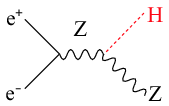
\includegraphics[width = 0.9\textwidth]{Pictures/Higgs/Chapter_Theory_figs_ZHdiagram.png}
            \caption{Higgs-Strahlung}
            \label{fig:higgsStrahlung}
        \end{subfigure}
        ~%\qquad
         %add desired spacing between images, e. g. ~, \quad, \qquad, \hfill etc. 
          %(or a blank line to force the subfigure onto a new line)
        \begin{subfigure}[t]{0.3\textwidth}
            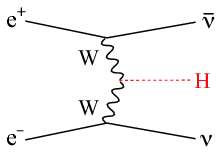
\includegraphics[width = 0.9\textwidth]{Pictures/Higgs/Chapter_Theory_figs_nunuHdiagram.png}
            \caption{$WW$-fusion}
            \label{fig:WW-fusion}
        \end{subfigure}
        ~%\qquad
         %add desired spacing between images, e. g. ~, \quad, \qquad, \hfill etc. 
          %(or a blank line to force the subfigure onto a new line)
        \begin{subfigure}[t]{0.3\textwidth}
            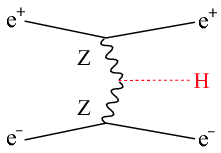
\includegraphics[width = 0.9\textwidth]{Pictures/Higgs/HiggsProd_eeH.png}
            \caption{$ZZ$-fusion}
            \label{fig:ZZ-fusion}
        \end{subfigure}
        \caption{Feynman diagrams of the main Higgs production at the ILC \cite{Asner2013}\cite{tian}.}
        \label{fig:higgsProduction}
    \end{figure}    
    
    The $WW$-fusion occurs only with left-handed electrons associated to right-handed positrons.
    Thus, by modifying the beam's polarisation, the signal mixture can be changed, as well as the background processes.

    \begin{figure}[!h]
      \centering
      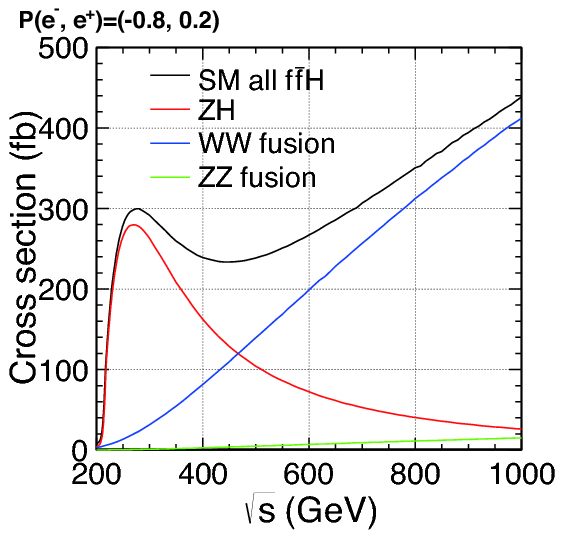
\includegraphics[width = 0.65\textwidth]{Pictures/Higgs/higgs_xsec_P-8_3.png}
      \caption{The cross section production of the Higgs boson with a mass of 125 GeV \cite{Asner2013}.}
      \label{fig:higgsXsec}
    \end{figure}

    \begin{figure}[!h]
      \centering
      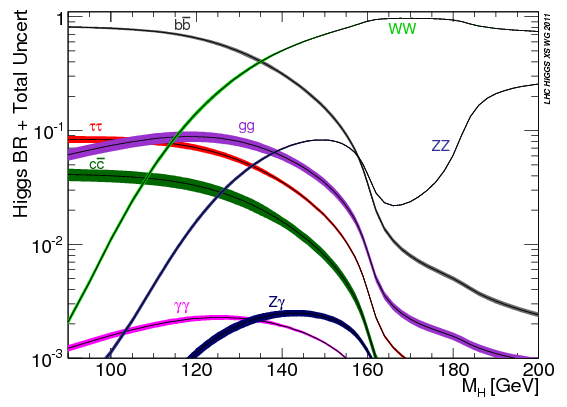
\includegraphics[width = 0.7\textwidth]{Pictures/Higgs/BRTotalUncertBands_lm.png}
      \caption{The Higgs boson branching ratio with the branching ratio uncertainties for the Higgs boson mass varying from $80$ to $200~\rm{GeV}$ \cite{Denner:2011mq}.}
      \label{fig:higgsProd}
    \end{figure}

    \subsection{Higgs boson studies}

    This section gives few ideas of possible Higgs boson physics studies.

    \subsubsection{Mass measurement}

    The first study will be at the peak production of the Higgs-strahlung. 
    The well defined four-momentum initial state allows to measure the Higgs boson mass regardless its decay products.
    The Higgs boson invariant mass $M_H$ can be calculated by using the recoil technique:

    \begin{equation}
      M^2_H = s + M^2_Z - 2 \sqrt{s}\left(E_{1} + E_{2}\right),
    \end{equation}

    where $M_Z$ is the mass of the $Z$ boson, $E_1$ and $E_2$ are the energy of the $Z$ decay products. 
    This technique works well for the $Z$ boson decaying into leptons at the centre-of-mass energy $\sqrt{s} = 250~\rm{GeV}$.
    However, this method can not be performed for a Higgs boson decaying into quarks at the same energy. 
    The $Z$ and the Higgs bosons are produced almost at rest, thus, the identification of the jets coming from the $Z$ boson to the ones coming from the Higgs boson is more difficult.
    Nevertheless, at higher energy ($\sqrt{s} = 500~\rm{GeV}$), the two bosons are enough boosted to separate their jets and then to apply again the recoil mass.
    Depending on the decay channel of the $Z$ boson, the statistical precision on the mass measurement varies between $40~\rm{MeV}$ (for $Z \rightarrow \mu^+\mu^-$) to $80~\rm{MeV}$ (for $Z \rightarrow e^+e^-$) and can reach $32~\rm{MeV}$ by combining the two results.

    \subsubsection{Spin measurement}

    At the thresholds production of the Higgs-strahlung ($\sqrt{s} = 250~\rm{GeV}$), besides the mass measurement, the determination of the spin and the CP-violation are scheduled.
    From the \gls{LHC} analysis, it has been determined that a spin-1 Higgs boson is forbidden because of the di-photon channel observation \cite{TheATLASCollaboration2013}.
    The spin will be determined by studying the Higgs-strahlung production mode.
    The cross-section has different behaviour, depending on the spin and the CP-violation.
    For a spin-0 and CP-even Higgs boson, the production cross-section follows $s$, whereas for CP-odd, it has a $\sqrt{s}^3$ dependency.

    \subsubsection{Branching ratio measurement}

    Although the decay $H \rightarrow b\overline{b}$ is the dominant decay mode of the Higgs boson at hadrons colliders, the existence of the boson was observed by studying the di-photons channel.
    \todo{H decays at LHC: bb, $WW$, tau tau, gamma gamma, gg and ZZ}
    %The Higgs boson discovered at the \gls{LHC} was observed by studying its decay to two photons.
    %At the \gls{LHC}, the decay $H \rightarrow b\overline{b}$ is observed under special kinematics. 
    The other decay states are challenging to separate from the background.
    The properties of the \gls{ILC} beam allow to perform measurements of the Higgs boson couplings to the particles defined in the \gls{SM}.
    Thus, the following decay modes are accessible: $b\overline{b}$, $WW$, $ZZ$, $gg$, $c\overline{c}$, $\tau \tau$, $\gamma \gamma$, $\gamma Z$.
    The observation of the $H \rightarrow c\overline{c}$ is one of the constraint parameter to build the detectors, specifically, the vertex detector that should be able to distinguish the vertices coming from the $b$-quarks to the ones coming from the $c$-quarks.
    Figure~\ref{fig:coupling} depicts the mass-coupling relation of the Higgs boson to the particles of the \gls{SM}.
    Any deviations from the Higgs boson fermionic coupling would indicate multiple states for the Higgs boson.\todo{Not clear enough}
%    The study of the Higgs fermionic coupling is a good test to know the nature of the Higgs.
%    The \gls{SM} nature of the Higgs boson will be tested by looking for any deviations from its fermionic coupling.
%    A deviation might indicate multiple states for the Higgs boson. \todo{Not clear enough}

    \begin{figure}[!h]
      \centering
      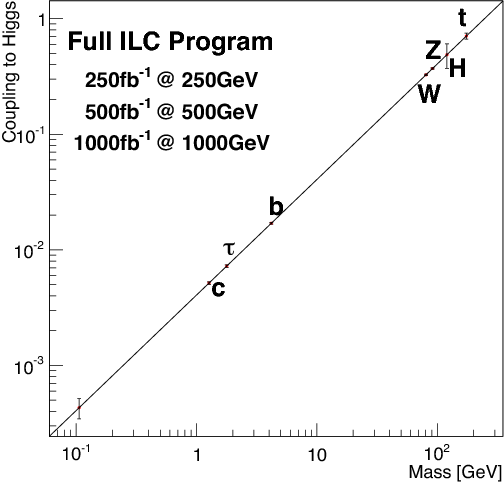
\includegraphics[width = 0.5\textwidth]{Pictures/Higgs/Chapter_Theory_figs_mass-coupling1TeV.png}
      \caption{Mass-coupling relation of the Higgs boson to the particles defined in the standard model \cite{tian}.}
      \label{fig:coupling}
    \end{figure}


  \section{Analysis of simulated data}
  
    Due to the restricted time to conduct the thesis, this section is introducing the tools to perform an analysis of simulated data at the ILD. 
    %The results shown here are not the last update and are already demonstrated \cite{Mueller}. 
    Nevertheless, the philosophy to perform a study of the Higgs boson production at the center-of-mass energy $\sqrt{s} = 350~\rm{GeV}$ and a luminosity of $250~\rm{fb}^{-1}$ is here presented.
  
  \subsection{Simulation set-up}  
  \label{subsec:ILCSOFT}

    The physics events are generated with Monte-Carlo simulation tools and is performed with different software.
    The collisions of electrons and positrons is done with the software WHIZARD \cite{WHIZARD}.
    It supports the \gls{SM} processes, as well as a large variety of BSM models.
    For linear collider physics, the beamstrahlung, the \gls{ISR} and the beam polarisation are simulated, but the hadronisation and fragmentation are not implemented and the simulation of this events was performed with PYTHIA \cite{PYTHIA}.
  
    The linear collider community has developed Monte-Carlo simulation and analysis software frameworks dedicated for a future linear collider, such as the \gls{ILC}. 
    The different packages developed by the community are grouped into the ILCSoft framework \cite{ilcsoft}.
    %The ILCSoft provides a large variety of software packages which were developed for the linear collider community\cite{ilcsoft}.
    It includes software for Monte-Carlo simulation, as software for test beam analysis (see chapter~\ref{chap:X0}) and other tools.
    The main package is the \gls{LCIO}, a persistence framework and event data model for the linear collider detector studies \cite{lcio}. 
    It provides a common data format and event data model for both the simulation studies and the analysis framework in order to share results and compare reconstruction algorithms.

    %The Monte-Carlo simulation is performed in three steps.
    %The first one consists to generate the physics events of electron/positron collisions.
    %The generation of Mont-Carlo events are performed with WHIZARD\cite{WHIZARD}.
    %This software includes \gls{SM} processes, as well as a large variety of BSM models.
    %For the purpose of the \gls{ILC}, it can simulate the beamstrahlung, the \gls{ISR} and the beam polarisation.
    %Although the hard interaction are simulated with WHIZARD, the hadronisation and fragmentation are implemented by using PYTHIA\cite{PYTHIA}.

    Afterward the physics events are generated, the particle interaction inside the detector is simulated with Mokka \cite{Mokka}.
    The software is based on GEANT4 simulation toolkit \cite{GEANT4} and is part of the ILCSoft.
    For the analysis, the detector model used is ILD\_o1\_v05.
    This model simulates the dead areas due to cabling, cooling system and mechanical structure and has a silicon-tungsten electromagnetic calorimeter, as well as an analog hadronic calorimeter.
    
    The detector geometry is described by a XML steering file and is used as an interface during the data reconstruction and analysis.
    This is managed by the \gls{GEAR} software \cite{GEAR}.

    Finally, the events are reconstructed with the \gls{Marlin} package \cite{MARLIN}.
    It is a C++ software framework used for the data reconstruction and the data analysis and it handles \gls{LCIO} data format.
    The different steps of the analysis or the reconstruction are grouped into modules, also called processors that read an input file, perform the defined tasks and write an output file that could be processes by another \gls{Marlin} module.
    A steering file written in XML is used to select the processors to use and the order of their execution time.

  \subsection{Event generation}
     
     \subsubsection{Event samples}

     The \gls{ILD} generator group has produced signal and background samples for two different polarisations:  $\mathcal{P}_{e^-,e^+} = (-1,+1)$ and $\mathcal{P}_{e^-,e^+} = (+1,-1)$.
     Although the scheduled polarisation are $\mathcal{P}_{e^-,e^+} = (-0.8,+0.3)$ and  $\mathcal{P}_{e^-,e^+} = (+0.8,-0.3)$, the simulated beam polarisation is re-weighted according to:
     
     \begin{equation}
       \begin{array}{lrc}
       \sigma_{\mathcal{P}_{e^-,e^+}} & = & \frac{(1 - P_{e^-})(1+P_{e^+})}{2} \sigma_{LR} + \frac{(1+P_{e^-})(1-P_{e^+})}{2} \sigma_{RL}, \\
       \sigma_{-0.8,+0.3} & = & 0.585 \times \sigma_{LR} + 0.035 \times \sigma_{RL}, \\
       \sigma_{+0.8,-0.3} & = & 0.035 \times \sigma_{LR} + 0.585 \times \sigma_{RL}.
       \end{array}
     \end{equation}

     The cross-section $\sigma_{LR}$ is for the polarisation $\mathcal{P}_{e^-,e^+} = (-1,+1)$, whereas $\sigma_{RL}$ is the cross-section of the polarisation $\mathcal{P}_{e^-,e^+} = (+1,-1)$.
     On the one hand, the Higgs-strahlung and the $WW$-fusion processes are equally important for the beam polarisation  $\mathcal{P}_{e^-,e^+} = (-0.8,+0.3)$, leading to a larger $\nu\overline{\nu} H$ cross-section.
     On the other hand, the polarisation $\mathcal{P}_{e^-,e^+} = (-0.8,+0.3)$ is used to perform a cross-check measurement.
     The $W$-boson cannot couple to right-handed electrons and left-handed positrons.
     Thus, the $WW$-fusion process is largely suppressed.
     Besides, the $Z$-boson depends on the isospin and the Higgs-strahlung contribution is also reduced but not suppressed.
     The same effect occurs on the backgrounds leading to a smaller background contamination on the signal and a cleaner signal sample for the Higgs-strahlung.

     The data set are scaled to an integrated luminosity of $250~\rm{fb}^{-1}$ for each beam polarisation.

  \subsubsection{Signal}

    The signal to study is the final state $\nu\overline{\nu}H$, on which the Higgs boson decays into a pair of quarks, such as $H \rightarrow b\overline{b}$ and $H \rightarrow c\overline{c}$, or a pair of gluons $H \rightarrow gg$. 
    The other decay modes are considered here as a source of background. 
    The dominant production processes leading to this final state are the Higgs-strahlung and the $WW$-fusion.
    Their leading order Feynman diagrams are displayed respectively on figure~\ref{fig:higgsStrahlung} and~\ref{fig:WW-fusion}.
    Although the neutrinos produced in the $WW$-fusion process are only $\nu_{\rm{e}}$ and all neutrino flavors are equi-probable in the Higgs-strahlung, the neutrino flavors cannot be detect and only the missing energy is the signature of neutrino production.

    \begin{figure}[!h]
      \centering
      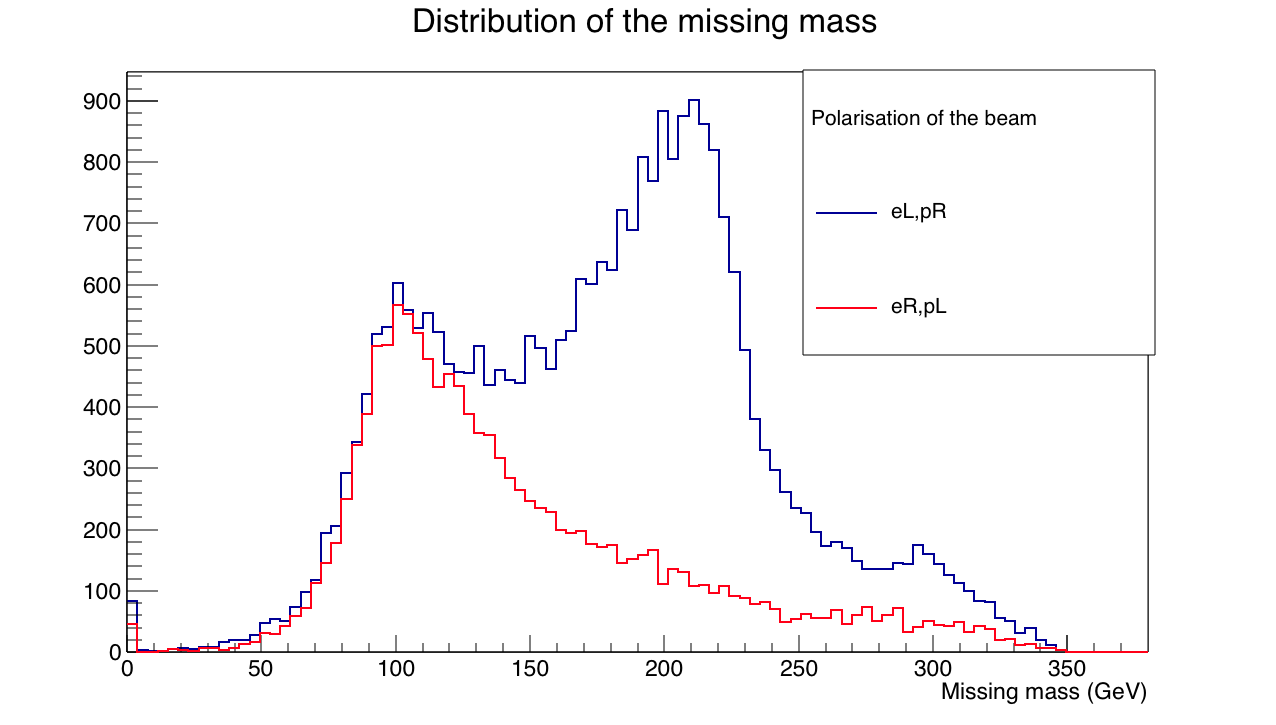
\includegraphics[width = 0.9\textwidth]{Pictures/Higgs/mMiss.png}
      \caption{Distribution of the missing mass with different beam polarisations and for the Higgs-strahlung and $WW$-fusion leading to $\nu\overline{\nu}H$ final state.
      The background contribution is not taken into account here.}
      \label{fig:mMiss}
    \end{figure}

    Figure~\ref{fig:mMiss} represents the distribution of the missing mass for the signal events for the two polarisations considered at the \gls{ILC}.
    The first effect of the polarisation is the suppression of the $WW$-fusion contribution and also a reduction of the Higgs-strahlung for right-handed electrons and left-handed positrons.
    For the other polarisation, the missing mass distribution shows three peaks. 
    Once centered around $90~\rm{GeV}$ corresponding to the decay of the Z-boson into a pair of neutrinos.
    The second peak is broader and its maximum is at $200~\rm{GeV}$.
    This comes from the $WW$-fusion.
    A third peak is visible at $300~\rm{GeV}$ and is coming from the Higgs boson decaying not hadronically and is considered as a source of background.    

  \subsubsection{Background processes}

    The signal hypothesis is that the final state is consisting of two jets coming from the hadronic decay of the Higgs boson, as well as missing energy coming from the undetected neutrinos produced by the $Z$ boson decay.
    Nonetheless, this signal is drown into the background processes.
    The background consists to the events with the same final states as the signal, called irreducible background and the events with a similar detector response.
    Their contributions depend on the beam polarisation.
    For example, the cross-section for a beam polarisation $\mathcal{P}_{e^-,e^+} = (+0.8,-0.3)$ is smaller by an order of magnitude due to the $W$ boson.

    Two irreducible backgrounds are considered here, the one involving a $W$-boson exchange and the one with a $Z$-boson exchange.
    The cross-section of this processes is few times larger than the signal one.
    For both, single $W$-boson and $Z$-boson exchange, the final state contains two jets with missing energy.
    Nevertheless, the final state with quarks is more likely than the final state with two gluons due to the loop formed in the final state on which the gluons are emitted.

    The background involving $W$-bosons, such as $e^{-}e^{+} \rightarrow W^{\pm}e^{\pm}\nu_{e} \rightarrow e^{\pm}\nu_{e}q\overline{q}$ is two orders magnitude bigger than the signal cross-section.
    The neutrino produced carries a large transverse momentum, whereas the electron or positron has a low transverse momentum.
    Hence, it can be undetected and be considered as a missing energy.
    
    The $W$-pair production can lead to semi-leptonic, hadronic and leptonic decay modes.
    The semi-leptonic mode consists of two jets and a lepton with its associated neutrino ($e^{+}e^{-} \rightarrow W^+W^- \rightarrow \nu_{l}l^{\pm}q\overline{q}$) and it is the major background process for the $W$-pair production.
    This background is detected by looking for an isolated lepton.
    Nevertheless, the lepton could escape the detector undetected or be inside a jet.
    The second $W$-pair production is the hadronic decay on which there is no missing energy ($e^{+}e^{-} \rightarrow W^+W^- \rightarrow q\overline{q} q\overline{q}$).
    This background is reduced by applying cuts on the missing momentum and the di-jet invariant mass.
    The last contribution is the leptonic final state, which is easy to distinguish from the signal.
    Thus, it is not considered in the study. 

    The $Z$-pair background is ten times smaller than the $W$-pair production.
    The  $e^+e^- \rightarrow ZZ \rightarrow \nu_{l}\overline{\nu_{l}}q \overline{q}$ process is an irreducible background.
    The hadronic decay $e^+e^- \rightarrow ZZ \rightarrow q\overline{q} q\overline{q}$ is reduced by cutting on the missing momentum and the di-jet invariant mass.
    The semi-leptonic process $e^+e^- \rightarrow ZZ \rightarrow l^+l^- q\overline{q}$ is easier to detect because of the second isolated lepton in the event.

    Finally, the last background to take into account is the one with the Higgs boson produced in the final state.
    The Higgs-strahlung can lead to $q\overline{q}H$ and $l^{\pm}l^{\mp}H$ has cross-section three times larger than the signal, but it is easily identify due to the absence of neutrino.
    All the decay mode of the Higgs boson different from $H \rightarrow b\overline{b}$, $H \rightarrow c\overline{c}$ and $H \rightarrow gg$ are considered as part of the background.

    \begin{figure}[!h]
      \centering
      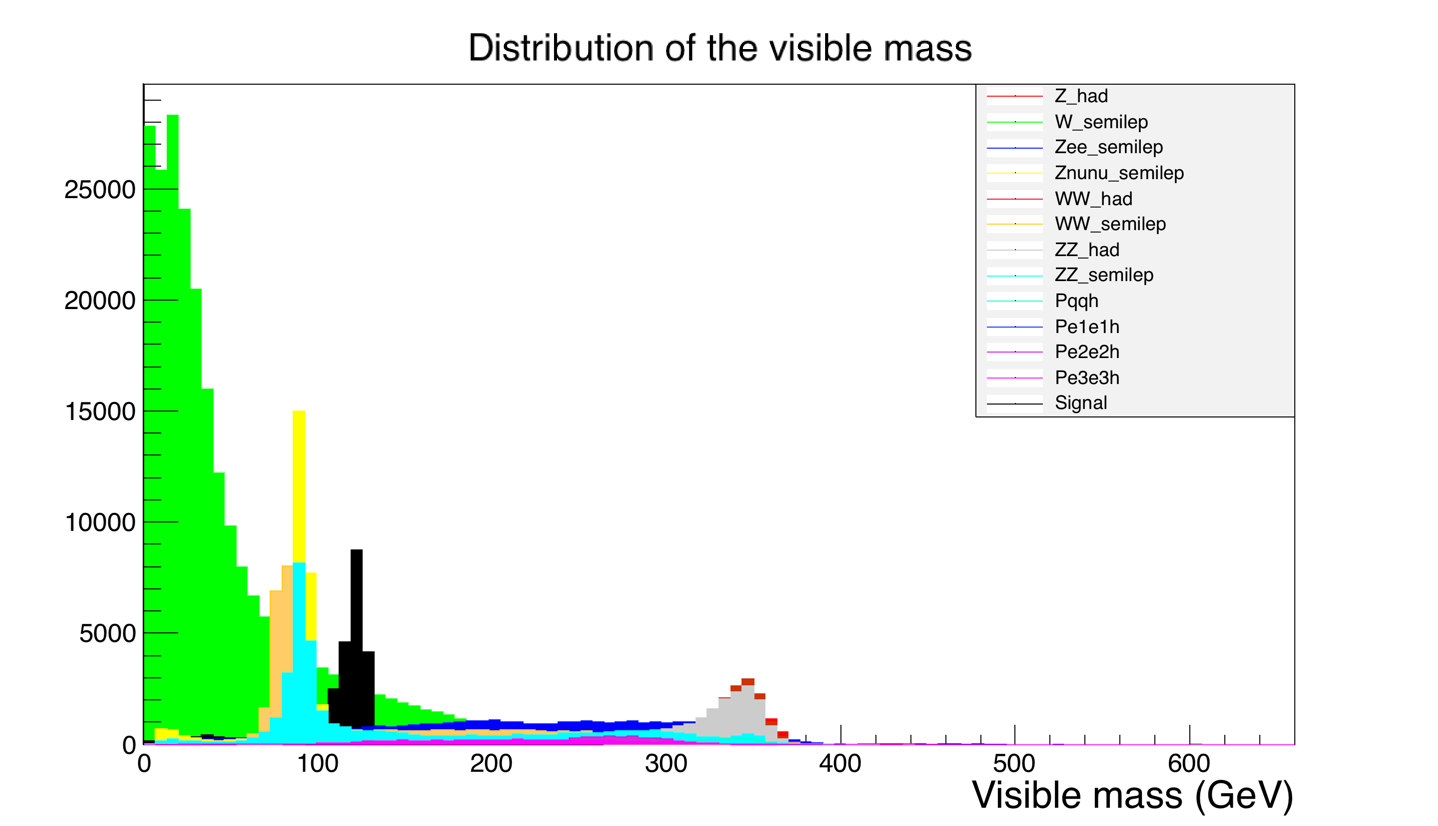
\includegraphics[width = 0.9\textwidth]{Pictures/Higgs/mVis_all.png}
      \caption{Distribution of the visible mass for the signal and background together and the polarisation $\mathcal{P}_{e^-,e^+} = (-0.8,+0.3)$.}
      \label{fig:mVisAll}
    \end{figure}

    Figure~\ref{fig:mVisAll} shows the distribution of the visible mass for all the processes taken into account during the analysis and a beam polarisation $\mathcal{P}_{e^-,e^+} = (-0.8,+0.3)$.
    A selection has to be performed in order to isolate the peak at $125~\rm{GeV}$.

  \section{Results}
 
    \subsection{Event reconstruction}

    The assumption to study the $H \nu\nu$ channel is to reconstruct a final state which is giving a two jets and missing energy in the detector response.
    The reconstruction consists to select and highlight this detector response.

    The first step consists to identify in the events the presence of isolated leptons in the final state and to remove them from the physics list.
    The lepton detected outside a jet are considered as a source of background.
    Thus, a neural network is used to identify in an event the different leptons and checks if they belong to a jet.
    This selection is based on different criteria, like the vertex information, the energy deposited inside the \gls{ECAL}, the \gls{HCAL} and the muon system. 
    The processor used for the identification is called \textit{IsolatedLeptonTagger} and has a veto efficiency of roughly $90~\%$.
    The $10~\%$ of leptons undetected are coming from events in which the leptons are moving into the forward region and they could escape the detector without being identify by the processor.
    A better selection is done after the jet reconstruction and is discussed later.

    A second source of background is coming from the $\gamma \gamma$ interactions which produce low $p_{t}$ hadrons.
    This hadrons with a small transverse momenta and a small relative angle to the beam axis are detected as jet-like objects in the forward region of the detector.
    The identification of the beam jets is based on the $k_{T}$ algorithm \cite{Cacciari2008}.
    It consists to define a "distance" $d_{ij}$ between two particles and to find the first closest constituent.
    
    \begin{equation}
      \begin{array}{lcl}
        d_{ij} & = & \frac{\rm{min}\left(p^2_{T_i}, p^2_{T_j}\right) \cdot \Delta R^2_{ij}}{R^2}, \\
        d_{i}  & = & p^2_{T_i},
      \end{array}
    \end{equation}

    with $\Delta R^2_{ij} = \left( y_{i} - y_{j}\right)^2 + \left( \phi_{i} - \phi_{j}\right)^2$, $y_{i}$ the pseudo rapidity, $\phi_{i}$ the azimuthal angle and $p_{T_i}$ the transverse momentum of the particle studied.
    The minimum between $d_{ij}$ and $d_{i}$ is calculated.
    If $d_{ij}$ is the minimum value, then, the particles $i$ and $j$ are merged into a jet candidate, they are then removed from the physics list and the jet candidate is added instead.
    If the minimum value is $d_{i}$, the particle is considered to be part of the beam jet and is removed from the particle lists.
    This algorithm is repeated iteratively until the number of jets created is equal to the number of jets expected.
   
    After removing the isolated leptons and the low $p_{t}$ hadrons from the physics list, the jet clustering and the flavor tagging processors are applied. 
    Because of the $k_{T}$ algorithm, which removes particle from the physics list, the vertex finder is run again before to use the jet clustering algorithm.

  \subsection{Event selection}

  To improve the signal to noise ratio, an event selection is performed by applying different cuts that reduce the background contribution.
  The order and the performances of the selection cuts are determined by maximising the significance $s$, which is:

  \begin{equation}
    s = \frac{\rm{N_{sig}}}{\sqrt{\rm{N_{sig}}+ \rm{N_{bg}}}},
  \end{equation}
  with, $\rm{N_{bg}}$ the number of remaining background and $\rm{N_{sig}}$, the number of remaining signal.
  The maximisation of $s$ is needed to minimise the statistical error.
  Firstly, the procedure starts with the definition of a collection of observables that could help to discriminate the signal from the background.
  Then, a test of the possible cut values is performed in a given range and for a given step size.
  The value leading to the largest significance is chosen as the optimum observable and is the first selection variable which is applied to a signal sample (containing $WW$-fusion and Higgs-strahlung processes) and the least tight constraint is selected in order to maintain a good signal efficiency.
  Finally, the cut values of this optimum observable is applied on the complete data set and the procedure is applied again.

  The first observable to be applied is the veto information used to find any isolated lepton.
  As already mentioned, the \textit{IsolatedLeptonTagger} processor has a veto efficiency of roughly $90~\%$. 

  The second observable is the visible transverse momentum $P_{\rm{t,vis}}$ of the di-jets. 
  \begin{equation}
    \begin{array}{lcl}
      P_{\rm{t,vis}} = \sqrt{P^2_{x,vis} + P^2_{y,vis}}, \\
      P_{\rm{x/y,vis}} = P_{\rm{x/y,j1}} + P_{\rm{x/y,j2}}. 
    \end{array}
  \end{equation}
 
  $ P_{\rm{x/y,j1}}$ and $ P_{\rm{x/y,j2}}$ are the visible momentum in the $x$ and $y$-directions for the two jets $j1$ and $j2$.

  The third observable is the invariant visible mass $m_{\rm{vis}}$, which is the signal signature.

  \begin{equation}
   \rm{m_{vis}} = \sqrt{E^2_{\rm{vis}} - \overrightarrow{P}^{\,2}_{\rm{vis}}},
  \end{equation}
  with $E_{\rm{vis}}$ and $P_{\rm{vis}}$ the visible energy and momentum of the event.
  The expected visible mass is $\rm{m_H} = 125~\rm{GeV}$ and its width is mainly driven by the jet energy resolution.

%    \begin{sidewaystable}
%    \scriptsize{
%    \flushleft
%      \begin{tabular}{c c c c c c c}
%           \hline
%           {Process} & {Cross Section (fb)} & {Events number} & \text{No isolated leptons} & {$35 <~\rm{{P}_{t}^{vis}} < 155~\rm{GeV} $} & {$95 <~\rm{m_{vis}}< 140~\rm{GeV}$} & {$-1 <~\rm{\cos{\alpha}}< 0.22$} \tabularnewline \hline
%           \hline
%           Zhad            &$ 3.86\times 10^{4} $&$	1.27\times 10^{7} $&$ 1.26\times 10^{7} $&$ 1.09\times 10^{5} $&$ 5.79\times 10^{2} $ &$	5.05\times 10^{2}  $\tabularnewline 
%           WW had          &$ 6.53\times 10^{3} $&$	2.16\times 10^{6} $&$	2.14\times 10^{6} $&$	5.27\times 10^{3} $&$	6.29              $ &$	6.29               $\tabularnewline 
%           WW semilep      &$ 8.16\times 10^{3} $&$	2.69\times 10^{6} $&$	1.17\times 10^{6} $&$	6.38\times 10^{5} $&$	1.13\times 10^{5} $ &$  6.26\times 10^{4}  $\tabularnewline 
%           ZZ had          &$ 6.01\times 10^{2} $&$	1.98\times 10^{5} $&$	1.97\times 10^{5} $&$	2.74\times 10^{3} $&$	1.20              $ &$  6.20\times 10^{-1} $\tabularnewline 
%           ZZ semilep      &$ 5.65\times 10^{2} $&$ 1.86\times 10^{5} $&$ 1.40\times 10^{5} $&$ 7.49\times 10^{4} $&$ 1.46\times 10^{4} $ &$  8.20\times 10^{3}  $\tabularnewline 
%           singleW semilep &$ 1.63\times 10^{3} $&$ 5.36\times 10^{5} $&$	2.24\times 10^{4} $&$	8.79\times 10^{3} $&$	1.65\times 10^{3} $ &$	1.63\times 10^{3}  $\tabularnewline 
%           singleZee semi  &$ 3.10\times 10^{2} $&$	1.02\times 10^{5} $&$	1.30\times 10^{4} $&$	2.17\times 10^{1} $&$	7.00\times 10^{-2}$ &$	7.00\times 10^{-2} $\tabularnewline 
%           singleZnn semi  &$ 3.55\times 10^{2} $&$	1.17\times 10^{5} $&$ 1.17\times 10^{5} $&$	8.38\times 10^{4} $&$	1.62\times 10^{4} $ &$	1.19\times 10^{4}  $\tabularnewline 
%           Higgs BG        &$ 1.62\times 10^{2} $&$	5.34\times 10^{4} $&$ 4.19\times 10^{4} $&$ 4.59\times 10^{3} $&$	1.93\times 10^{2} $ &$	1.43\times 10^{2}  $\tabularnewline 
%           HiggsToOther    &$ 3.05\times 10^{1} $&$	1.01\times 10^{4} $&$	6.66\times 10^{3} $&$	4.95\times 10^{3} $&$ 3.45\times 10^{3} $ &$	2.64\times 10^{3}  $\tabularnewline 
%           \hline						
%           Background     &$ 5.69\times 10^{4} $&$  1.88\times 10^{7} $&$	1.65\times 10^{7} $&$	9.31\times 10^{5} $&$ 1.50\times 10^{5} $ &$  8.76\times 10^{4}  $\tabularnewline 
%           Signal	        &$ 6.82\times 10^{2} $&$  2.25\times 10^{4} $&$	2.23\times 10^{4} $&$	1.82\times 10^{4} $&$	1.66\times 10^{4} $ &$	1.57\times 10^{4}  $\tabularnewline 
%           Significance   &                     &$	5.19              $&$	5.48 $             &$	1.87\times 10^{1} $&$	4.06\times 10^{1} $ &$  4.88\times 10^{1}  $\tabularnewline 
%     \end{tabular}
%    }
%    \caption{Cut flow chart with three first cuts applied.}
%    \label{tab:cutFlow}
%  \end{sidewaystable}

  \begin{table}
    \begin{tabular}{c c c c}
      \hline
      Process                                     & Background          & Signal              & Significance  \tabularnewline
      \hline
      \hline
      Cross-section (fb)                          & $5.69 \cdot 10^{4}$ & $6.82 \cdot 10^{2}$ &               \tabularnewline
      \hline
      Expected event number                       & $1.88 \cdot 10^{7}$ & $2.25 \cdot 10^{4}$ & $5.2$         \tabularnewline
      No isolated leptons                         & $1.65 \cdot 10^{7}$ & $2.23 \cdot 10^{4}$ & $5.5$         \tabularnewline
      {$35 <~\rm{{P}_{t}^{vis}} < 155~\rm{GeV} $} & $9.31 \cdot 10^{5}$ & $1.82 \cdot 10^{4}$ & $18.7$        \tabularnewline
      {$95 <~\rm{m_{vis}}< 140~\rm{GeV}$}         & $1.50 \cdot 10^{5}$ & $1.66 \cdot 10^{4}$ & $40.6$        \tabularnewline
      {$-1 <~\rm{\cos{\alpha}}< 0.22$}            & $8.76 \cdot 10^{4}$ & $1.57 \cdot 10^{4}$ & $48.8$        \tabularnewline
      $26 < (\rm{N.R.C > 1GeV}) < 99$             & $2.25 \cdot 10^{4}$ & $1.19 \cdot 10^{4}$ & $56.3$        \tabularnewline
      $0.11 < \rm{DurhamjD2ym} < 1$               & $1.78 \cdot 10^{4}$ & $1.05 \cdot 10^{4}$ & $62.3$        \tabularnewline
      $0 < \rm{abs(RefinedjPzvis)} < 113~\rm{GeV}$& $1.51 \cdot 10^{4}$ & $1.01 \cdot 10^{4}$ & $63.5$        \tabularnewline
      $156 < \rm{RefinedjEmiss} < 230~\rm{GeV}$   & $1.37 \cdot 10^{4}$ & $9.85 \cdot 10^{3}$ & $64.1$        \tabularnewline      
      \hline %----------------------------
    \end{tabular}
    \caption{Cut-flow table for a beam polarisation $\mathcal{P}_{e^{-},e^{+}} = (-0.8, +0.3)$.}
    \label{tab:cutFlow}
  \end{table}

  Table~\ref{tab:cutFlow} summarises the order of the different cut selection for different observables applied on the simulated data set.
  After eight consecutively cuts, the background contribution is three orders smaller, whereas the signal is almost one order smaller than the beginning.
  Nevertheless, the significance is still less than 70 and applying more cuts is affecting strongly the signal.

  \section{Outlooks}

  To preserve the sample quality, it is rather better to use a \gls{MVA} method to extract the signal from the background.
  The complete information is then used simultaneously to find the best sets of variable.
  This analysis was already performed and a \gls{MVA} method was used, achieving a significance above $70$.

  The next step of this analysis is to focus on the decay mode of the Higgs boson into two pairs of charmed quarks and to optimise the flavor tagging performances to separate more accurately the $b$ and $c$ quarks events.
  For the events and the detector simulated in this chapter, the vertex detector geometry was not optimised and was made of five single sided layers.
  Nevertheless, the double sided option has to be investigated.
  This geometry offers multiple possibilities, like using two different types of sensors on the same ladder or the possibility of two point measurements per ladder for a track.
  One side could be equipped with ultra-fast integration time ($\mathcal{O} \sim 1~\rm{\mu s}$) sensors, whereas the other side could embed sensors with an excellent pointing resolution ($\sigma_{\rm{s.p}} \leq 3~\rm{\mu m}$).
  With two sensors on the same mechanical structure, a track is reconstructed by two points of measurement.
  Thus, these two measurements could be combined together to form "mini-vectors".
  Studying the "mini-vectors" could help to identify the beam-strahlung from the collision events.



  %This is important to determine the geometry configuration and the technology used to build the vertex detector.
  %The study could consist first to compare the branching ratio measured with two different detector geometries. 
  %The one used in this analysis was made of a five single sided layers, but to decide which structure, like single or double-sided ladder, the analysis as to be ran again.
  %One possible vertex detector considered is made of three double-sided layers.
  %On one side of a ladder, sensors with an ultra-fast integration time ($\mathcal{O} \sim 1~\rm{\mu s}$) and on the other side, sensors with an excellent pointing resolution ($\sigma_{\rm{s.p}} \leq 3~\rm{\mu m}$).



    \chapter{Double-sided VXD: PLUME}
\label{chap:vxd}
  
  Since the end of the 1960's, the development of position sensitive silicon sensors has permitted to confirm the prediction of the \acrfull{SM} with a high precision, as well as the discovery of the top quark.
  These sensors, called \acrfull{VXD}, are in charge to track the particles down to their decay vertices.
  The design of such device is driven by the physics requirement of the experiment and is playing a crucial role at the \acrfull{ILC}.
  For example, one flagship measurement is the study of the Higgs boson couplings to the fermions and other bosons.
  This can be achieved only with a precise heavy flavor tagging and the ability to separate the $b$ quarks from the $c$ quarks. 
  Actually, the lifetime of the two quarks is of the same magnitude ($1.3 \time 10^{-12}~\rm{s}$ for the $b$ quark and $1.1 \time 10^{-12}~\rm{s}$ for the $c$ quark), leading to very close decay vertices. 
  
  Along this chapter, the role of the vertex detector and the physics requirements to develop one for the \gls{ILC} environment will be presented.
  Then, the different options of the \acrfull{ILD} are shown, to focus on the double-sided ladders developed by the \gls{PLUME} collaboration.
  To finish, the principle of \gls{CMOS} sensors and their use in physics are described.

  \minitoc
  
  \section{The ILD vertex detector specifications}
   
    The \gls{VXD} is the closest sub-detector to the \acrfull{IP} in charge of reconstructing the vertex by extrapolating particles back to their origin of production. 
    This detector should be optimised to track particles in a high-density environment and to be able to extract the tracks from the different particles, especially the $b$ and $c$ quarks in the case of the \gls{ILC}.
    The reconstruction of the displaced vertices should be efficient enough to perform a good flavour tagging.
    Therefore, the detector has to measure particles with a lifetime in the picosecond regime, representing a decay length between 150 and $500~\rm{\mu m}$.
    The minimum distance of the first \gls{VXD} layer is determined by the beam pipe radius, and the background induced by beamstrahlung, to limit the pixel occupancy.
    This sub-detector has a central role in the tracks' reconstruction.
    Depending on the option chosen, the \gls{VXD} has to provide five or six points of measurement with a very high precise spatial resolution.
    For the studies requiring vertex charge identification, it should be able to reconstruct low-momentum and very forward tracks.
    %The typical parameters of such detector are their thickness, especially their material budget to reduce unwanted interaction, and their pitch which defines the spatial resolution that can be achieved.

   \subsection{Physics requirements}


   
   The ideal \gls{VXD} should be made of sensors with a fine granularity in order to increase the ability to distinguish two nearest particles.
   The mechanical structure of the detector should provide a good stiffness and stability of the whole system but has to be at the same time as light as possible to reduce the interaction of the particles traversing it, before they reached another part of the main detector.
   As well, in order to reduce the unwanted interactions, the sensor technology used has to have a low power consumption to avoid any special cooling system which can have a bad impact on the material budget.
   The design of such detector, like the minimal distance of the first layer to the \gls{IP} and the spacing between different layers, is determined by both the beam background and the physics to study.
   The flavour tagging ability, the vertex charge measurement and tracking, and the displaced vertices reconstruction are the main physics parameters driving the design.
   %The structure should be as light as possible to minimize the interaction of particles before they are flying to the other detectors.
   %The distance of the first layer to the \gls{IP} should be as slow as possible and the power consumption should 
   %The first layer has to be as close as possible to the \gls{IP} and the lowest power consumption as possible
   %The flavour tagging ability, vertex charge measurement and track and displaced vertices reconstruction are the main physics parameter that is driving the design of such detector.
   The distance of closest approach of a particle to the colliding beam is called the impact parameter and the resolution achievable by the detector is described by the formula~\ref{eq:resIP}\cite{Battaglia2011}.
   %The resolution on the impact parameter $\sigma_{IP}$, defined as the distance of closest approach of the particle to the colliding beam can be parametrised by the formula~\ref{eq:resIP}.\todo{REPHRASE}
    
    \begin{equation}
      %\sigma_{IP} = 5 \mu\text{m} \oplus \frac{10 \ - \ 15 \mu\text{m}}{p \sin{\theta}^{3/2} }
      \sigma_{IP} = a \oplus \frac{b}{p \sin{\theta}^{k}}~\rm{,~with~k~=}
      \left\{
        \begin{array}{r l}
          \frac{3}{2} & \text{in the } R - \Phi \text{ projection,} \\
          \frac{5}{2} & \text{in the z projection.}
        \end{array}
      \right. 
      \label{eq:resIP}
    \end{equation}

    Where $\theta$ is the track polar angle, $a$ and $b$ are explained in the following.

   The first term $a$ is the impact parameter resolution of the sensors used for the \gls{VXD}, which is linked up to the radius of the inner $R_{\rm{int}}$ and outer $R_{\rm{ext}}$ layers and the single point resolution $\sigma_{s.p.}$, as described in equation~\ref{eq:aTerm}.

   \begin{equation}
     a = \sigma_{s.p}\frac{R_{\rm{int}} \oplus R_{\rm{ext}}}{R_{\rm{ext}} - R_{\rm{int}}}
     \label{eq:aTerm}
   \end{equation}

    In the case of the \gls{ILD}, the single point resolution should not be higher than $\sigma_{sp} \simeq 3~\rm{\mu m}$, leading to an impact parameter with a resolution of the order of $a \simeq 5~\rm{\mu m}$.
   
    The second term, $b$, presented in the equation~\ref{eq:bTerm}, is related to the multiple scattering inducing an uncertainty on the impact parameter.
    It depends on the charge $Z$ of the impinging particle, the material crossed by the particle $\frac{x}{X_0 \sin{\theta}}$ and the distance of the innermost layer to the \gls{IP}.
    Depending on the momentum or the crossing angle of the incoming particles, the two parameters are more or less important.
    For low momentum particles or crossing particles with a shallow angle, the $b$ parameter becomes important, while for higher momentum $a$ dominates.


    \begin{equation}
      b = R_{int} \frac{13.6 MeV/c}{\beta c}  Z \sqrt{\frac{x}{X_{0}}} \left[ 1 + 0.036 ln \left( \frac{x}{X_{0}\sin{\theta}} \right) \right].
      \label{eq:bTerm}
    \end{equation}
   
   For the \gls{ILC} purpose, the \gls{ILD}-\gls{VXD} should reach an impact parameter resolution better than $5~\rm{\mu m}$ and a $b$ parameter better than $10~\rm{\mu m~GeV/c}$. 
   This precision on these parameters were never obtained before in other experiments.
   %The values were never obtained before for other experiments. 
   As a comparison, the resolution parameters for the \gls{LHC} are: $a =  12 \ \mu$m and $b = 70 \ \mu$m GeV/c. 

   \subsection{Layout of the vertex detector}

   The \gls{VXD} will be made of 12 cm long ladders arranged cylindrically in concentric layers to form long-barrels surrounding the \gls{IP}, contrary to the \gls{SiD} vertex detector with a design based on a 5 layers barrel, four endcap disks and three additional forward pixel disks\cite{Behnke2010}.
   Two different geometries are under consideration for the \gls{ILC}-{ILD}, nevertheless, they are both based on long ladders. 
   The first option is based on five single-sided layers with a material budget not exceeding 0.11 \% of $X_0$ per layer.
   The five layers are in a radius range varying from 15 mm for the first layer to 60 mm for the last one.
   The second option is based on three double-sided layers.
   The material budget should be less than 0.16 \% of $X_0$ for one detecting face.
   The mechanical structure, which holds the two layers, is 2 mm thick and will be in a radius range varying from 15 to 60 mm.

   
  %  whereas the second one is based on three double-sided layers.
  % The material budget to be reached is 0.11 \% of $X_0$ per layer for the single-sided option and 0.16 \% of $X_0$ per layer for the double-sided.
  % The radius of the first layer depends strongly on the beam background as it is the first layer which is the most impacted.
  % For the single-sided option, the idea is to have five layers with a radius range from 15 to 60 mm.
  % The material budget per layer should be better than 0.1 \% of $X_0$.
  % The second option is made of three double-sided layers with a radius range from 16 to 60 mm.
  % The material budget for each detecting face should not exceed 0.16 \% of $X_O$.
  % At the moment the mechanical structure that holds the two layers is 2 mm thick, but some geometry optimisation depending on the physics to study might consider having closer layers on the first ladder, while the last ladder could have a thicker mechanical structure.
   
   \begin{figure}[!h]
     \centering
     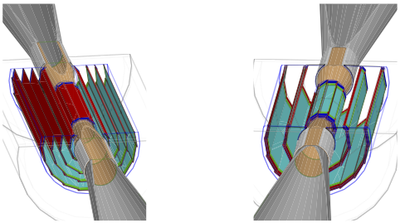
\includegraphics[width = 10 cm]{Pictures/vxd/ild_VXD.png}
     \caption{Overview of the two vertex detector option for the ILC. On the left, it is made of five single sided layers, whereas the right one represents three double-sided layers.}
   \end{figure}
   
   %They are two different geometrical designs understudied to build the \gls{VXD}. 
   %The first idea is to have a \gls{VXD} with five single-sided layers with a radii range from 15 to 60 mm.
   %The other option is to have three double-sided layers, which will have pixel sensors on both sides separated by a mechanical structure of 2 mm thickness. 
   %The radii range is from 16 to 60 mm.

   Both geometry designs are based on  pixel sensors instead of strips detectors.
   A non-exhaustive list of the possible technologies are presented below:
    
   \subsubsection{FPCCD}
   
     The \gls{FPCCD} \cite{CalanchaParedes} is based on the \gls{CCD} processes.
     The sensor is using small pixels size (approximately $\sim 5 \mu\text{m}$) to provide a sub-micron spatial resolution and an excellent capability to separate two nearby tracks.
     Its thickness is 50 $\mu\text{m}$ and the epitaxial layer (15 $\mu\text{m}$ thick) is completely depleted to limit the charge spreading around pixels and to reduce the number of hits per pixel.
     However, the \gls{CCD} architecture provides slow readout and the matrix will be read between consecutive bunch trains, helping to reduce the power consumption and avoiding beam induced RF noise.
     The \gls{FPCCD} are planned to be operated at $-40 \degres$C.

   \subsubsection{DEPFET}
    
    The \gls{DEPFET} \cite{Richter2003} is an \gls{APS} in which field effect transistors are incorporated into each pixel.
    The single point resolution is $\sim 3$ $\mu\text{m}$ for pixels with a size of 20 $\mu\text{m}$.
    The silicon itself is used as sensitive part but also as a mechanical structure, minimising the support and services.
    The sensor is completely depleted of free charged carries thanks to a voltage applied to the thickness.
    The rolling-shutter approach is used for reading each row and the column readout is done by two auxiliary \glspl{ASIC}.

    The \gls{DEPFET} technology is the one chosen  to build the vertex detector of the BELLE-II experiment\cite{depfetBelleII}.

    %Rapid and efficient collection of signal on a deep implant underneath the field effect transistor
    %Inside pixel: first amplification of signal
    %Columns readout by two auxiliary \glspl{ASIC} while rows read out in rolling shutter mode.

   \subsubsection{CMOS}

   Different options for \gls{CMOS} pixel sensors are studied, such as the 3D integrated \gls{CMOS}, but due to the context of this thesis, the work will focus on the \gls{CMOS} sensors based on the \gls{MIMOSA} architecture developed by the IPHC of Strasbourg. 
   This technology is described in section~\ref{sec:CMOS}.
  % The STAR experiment at RHIC is the first one to get an entire vertex detector made of ULTIMATE-MIMOSA28 CMOS sensors.
   %One of the technology developed is described in section~\ref{sec:CMOS}.

   For all the technologies, the sensors' power consumption has to be minimised in a way to reduce the cooling system and in the same time the added material budget in the sensitive detector volume.
   As it was shown on the figure~\ref{fig:bunches} of the chapter~\ref{chap:ILC}, the bunch train will last less than 1 ms for a dead time of 200 ms.
   Two possibilities are envisaged to benefit from the beam structure.
   The first one consists to store the hits information thanks to a time stamp during the bunch crossing and to read out the data after the last collision.
   This method might be used by the \gls{FPCCD} technology due to the slow integration time of the \gls{CCD}.
   Another solution is to use power-pulsing.
   Right after the last collision, the sensors are switched off or the power consumption is reduced as mush as possible, and before the first collision, the sensors is switch on again.
   This pulsing method is studied by different collaborations. 
   
   Another aspect not discussed yet is the radiation tolerance of the detector, which is directly related to the beam background.
   The first layer is the most affected by the background and it should have a high radiation tolerance. 
   The required radiation tolerance is about 1 kGy for the total ionising dose and a fluence of $10^{11}\text{n}_{eq}\text{/cm}^2$\cite{Behnke2013}.

   The efficiency of the \gls{VXD} has also to be excellent in order to maximise the tracking performances.
   The efficiency is defined here as the ratio of detected particles over all the particles crossing the detector.
   If one layer of the vertex detector misses a hit, the track reconstruction will be less accurate 
   
   % the vertex detector optimisation can be only achieved by taking into account the beam structure.
   %As it was shown on the figure~\ref{fig:bunches} of the chapter~\ref{chap:ILC}, the bunch train will last less than 1 ms for a dead time of 200 ms.
   %Instead of reading the data during the bunch train, the sensors can be read out right after the end of the bunch train, then they can be switched off, or reduce their consumption as mush as possible, and they can be switched on at their nominal working value right before the first collisions. 
   %This dead time can also be used to cool down the system.
   %Indeed, the cooling system add an additional material 
  
   
   

   \todo{Cooling system, integration time, radiation tolerance, electromagnetic interference}

   To summarise, the expected parameters expected for the \gls{ILC} are: 
   \begin{itemize}
     \item An excellent impact parameter resolution: $ a \sim 5 \mu\text{m}$ and $b \sim 10 \mu\text{m}$
     \item A material budget not exceeding 0.1 \% $X_0$ per layer for the single-sided option (0.16 \% $X_0$ for the double one)
     \item Radius of the first layer $\sim$ 15/16 mm
   \end{itemize}

  \section{PLUME}

  The \acrfull{PLUME} project aims to produce double-sided ladder prototypes with respect to the \gls{ILC} requirements\cite{PLUME}.
  Three labs in the Europe are involved: the IPHC-PICSEL in Strasbourg, the University of Bristol and DESY in Hamburg.
  The collaboration is studying the feasibility to build such vertex detector using \gls{MAPS} thinned down to $50 \mu\text{m}$ and is exploring the benefits of this design.
  Strasbourg is in charge to develop and mount the sensors on the modules, to take care of the readout and the \gls{DAQ}, and to provide a cooling system.
  The mechanical design, stability measurements and building the ladders are done by the University of Bristol, while DESY has studied the ladder mock-up, performed power-pulsing tests and is now characterising and validating the modules in the lab.
  In 2016, DESY has provided the opportunity to test the ladder in real conditions thanks to the test beam facility and the possibility to use the \gls{DAQ} software developed at DESY: EUDAQ\todo{REF: EUDAQ}.

    \subsection{Design and goals}

    The figure~\ref{fig:PLUME} illustrates the design of a PLUME ladder.
    The ladder structure is defined by the sensors arrangement on the mechanical structure (positioned next to each other).
    In this design, the stiffener is a 2 mm thick \gls{SiC} foam which has a density varying between 8 \% and 4 \% (depending on the ladder version) and could be reduced to only 2 or 3 \%.
    %The mechanical structure is made of a 2 mm thick silicon carbide foam which has a density varying between 8\% for the prototype build before 2011 and 4\% for the new ones.
    The choice of this foam is a good compromise between the stiffness and the thickness compare to other materials. \todo{REF Joel paper}
    The figure~\ref{fig:SiC} is representing the structure of this foam.
    It is macroscopically uniform and has the advantage to be easily machinable.
    Nevertheless, it has a low thermal conductivity (50 W/m/K) and can't be used to dissipate the heat.
    On each side, a low mass flex-cable is glued, which is used to connect the sensors for powering and managing them.
    It is made of copper traces coated in Kapton, but new prototypes using aluminum traces are developed and currently tested in order to reduce the material budget.
    %It is made of copper traces (prototype before 2011) or aluminum traces (new prototypes) coated in Kapton. 
    The ladder embeds twelve sensors, six on each face, that are glued and connected to the flex cable.
    On one edge of the flex-cable, a single \gls{ZIF} connector is used to link the ladder to the external board servicing, via a jumper cable.
    For the moment, the design is dedicated to the MIMOSA-26 sensors thinned down to $50 \mu\text{m}$ but it can be adapted to any kind of \gls{MAPS} sensors having the same thickness. 
    Although the MIMOSA-26 has a spatial resolution better than 3$\mu$m (see subsection~\ref{subsec:Mi26}), the integration time is not suited for the bunch train structures of the \gls{ILC}.

    The aims of the collaboration are to build ladders with a material budget better than 0.35\% of $X_0$ for a spatial resolution better than 3$\mu$m, and thus to evaluate the benefits of a double-sided measurement.

    \begin{figure}[!h]
      \centering
      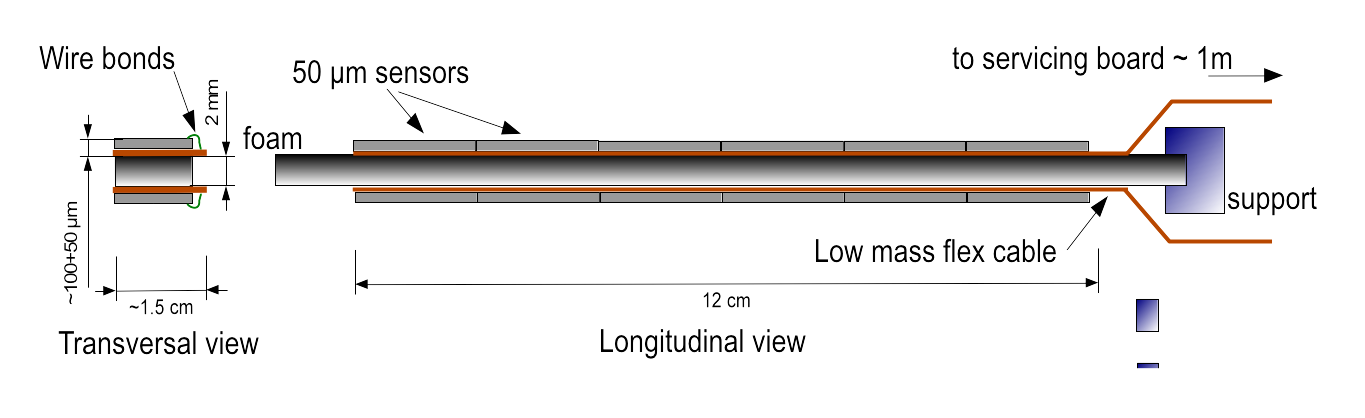
\includegraphics[width = 15 cm]{Pictures/vxd/plume_finalGoal.png}
      \caption{Side view (transversal and longitudinal) of the PLUME mechanical structure.}
      \label{fig:PLUME}
    \end{figure}

    \begin{figure}[!h]
      \centering
      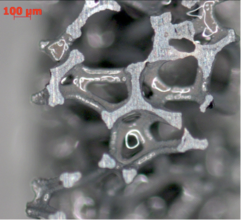
\includegraphics[width=0.3\textwidth]{Pictures/vxd/foam2.png}
      \caption{Microscopical view of the silicon carbide foam structure.}
      \label{fig:SiC}
    \end{figure}

    \subsection{Prototypes}

    Since 2009, the collaboration is studying the design, the production, the impact of the mechanical structure on the ladder's performances, but also how to power and control the sensors together.
    The first ladder prototype, called version-0 (V-0) was developed and tested in 2009.
    The purpose of this prototype was to settle the fabrication and the test beam procedures, without trying to reach the desired material budget goal.
    Two MIMOSA-20 analog output sensors were mounted on each side of a stiffener, providing a $1 \times 4 \text{ cm}^2$ sensitive area.
    The prototype was tested in 120 GeV pion beam at the CERN-SPS and the results have demonstrated the benefits of the double-sided measurement on the spatial resolution, which is improved by about 25\%\cite{Nomerotski}.

    Then in 2010, a second prototype featuring a design closer to the wanted goal, called version-1 (V-1), was developed.
    Each module of the ladder was made of Kapton flex-cable with a thickness of 0.14 mm, using copper traces.
    They are denoted \gls{OKF}, where Optiprint is the vendor of these flex-cable.
    It is the first version to embed six MIMOSA-26 binary output sensors working simultaneously on each side of the stiffener.
    The material budget is estimated to be 0.65 \% of $X_0$ in the sensor's sensitive area. 
    The aim of this prototype was to validate the operation of multiple sensors in a chain.
    Two ladders were tested in real conditions.
    The first one was tested with 120 GeV pions at CERN-SPS in 2011, while the second ladder was tested in April 2016 with up to 5 GeV positrons at DESY in Hamburg. 
    The DESY test beam results are presented in chapter ???, while a specific study of the sensor's deformation observed at CERN is discussed in chapter ???.

    \begin{figure}[!h]
      \centering
      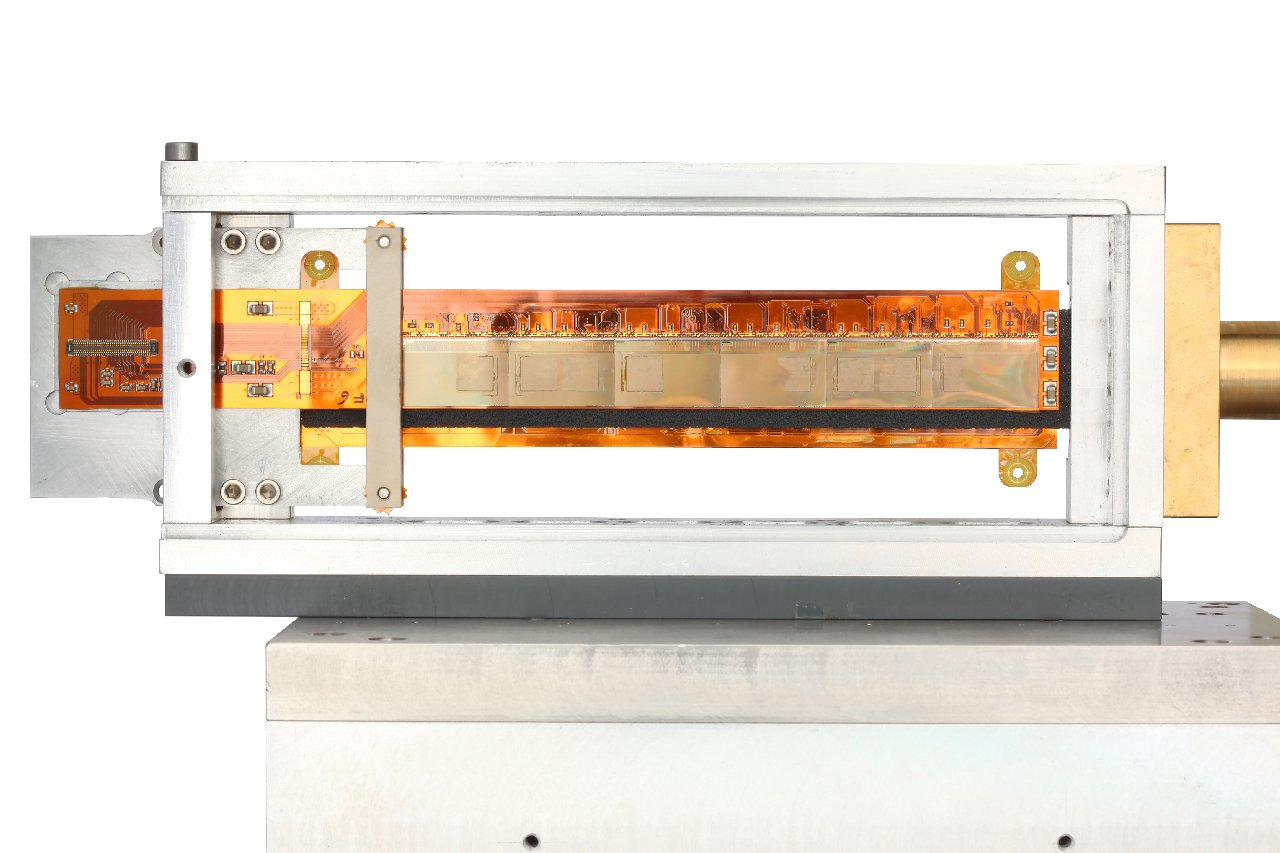
\includegraphics[width = 12 cm]{Pictures/vxd/plume_ladder2010_frontView}
      \caption{Front view of the ladder version-1 made in 2010 in its holding box. On the left, there is the connector to the output board servicing, on the right a connection to blow air on the module. As this version was not made with a mirrored design, the flexible cables are not entirely overlapping and the SiC foam can be seen (in black here).}
    \end{figure}

    At the beginning of 2016, the third prototype versions were mounted but have not yet been completely tested.
    In fact, this new version is divided into two sub-versions: one using copper traces and the other one aluminum traces.
    Nevertheless, both sub-versions have a new design featuring reduced traces thickness to have a narrower flex-cable (18 mm width) adjusted to the sensors width in order to minimise the dead areas.
    The flex-design has slightly changed to have a mirrored geometry (figure~\ref{fig:AM01}) and a straight geometry in order to minimize the dead area too and have a better alignment solution.
    The stiffener is made of a lower density \gls{SiC} foam reducing the global material budget. 

    \begin{figure}[!h]
      \centering
      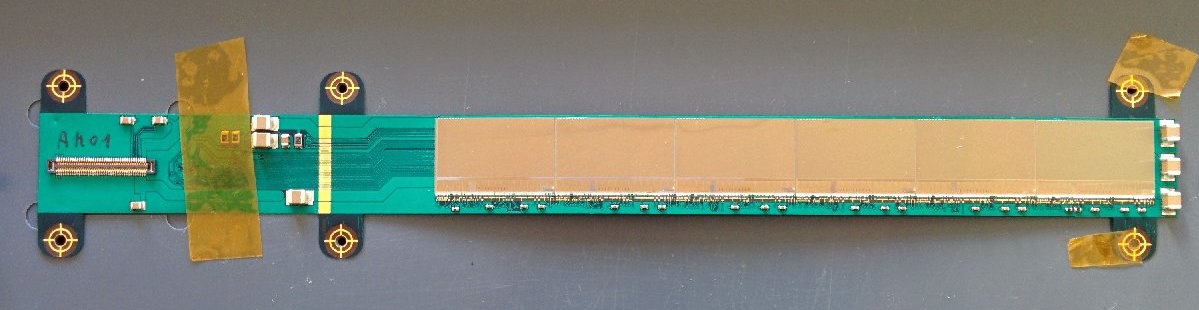
\includegraphics[width = 12cm]{Pictures/vxd/AM01.jpg}
      \caption{Picture of the first mirrored module made with aluminum traces. The cable width is adjusted to the size of the sensor.}
      \label{fig:AM01}
    \end{figure}
    The table~\ref{tab:X0} summarises the material budget reached by the different prototypes.

    %Before to reach the lightest ladder with a material budget of only 0.35 \%, the collaboration has studied the design, production and impact of the mechanical structure, but also how to power and control the sensors.
    
    %%The first ladder prototype (here labeled V0) was developed and test in 2009.
    %It has two MIMOSA-20 analog output sensors on each side of a stiffener, providing a $1 \times 4 \text{ cm}^2$ sensitive area.
    %As the purpose of this prototype was to settle the fabrication and the beam test procedure, the sensors and the flex-cables were not optimised.
     
    %The second prototype featuring the final device design (V1) was developed in 2010. 
    %The material budget is estimated to be 0.65 \% of $X_0$ in the sensor's sensitive area. 
    %It is the first version to embed six MIMOSA-26 binary output sensors on each side of the stiffener that were working simultaneously.
    %Two ladders were tested, one with 120 GeV pions at CERN-SPS in 2011 and the second one with positrons up to 5 GeV at DESY.
    %The test beam at DESY is presented in chapter ... and some results of sensor's deformation observed at CERN are discussed in chapter ...

    %The third prototype was mounted at the beginning of 2016 and has not been yet tested. 
    %The traces thickness was reduced, the flex-cable width was adjusted to the sensors width and the stiffener was made of a lower density Silicon Carbide foam reducing the material budget and the dead areas.

    \begin{table}
      \begin{center}
        \begin{tabular}{c c c c c c c}
        \hline %----------------------------
        \multirow{2}*{Layer}  & \multicolumn{3}{ c }{budget (\% X$_0$)}  \tabularnewline
                              &  V-0 & V-1 & Goal \tabularnewline
        \hline %----------------------------
        \hline %----------------------------
        Sensor                & 0.053 & 0.053 & 0.053 \tabularnewline
        Flex-cable            & 0.524 & 0.150 & 0.034 \tabularnewline
        Passive components    & 0     & 0.033 & 0.033 \tabularnewline
        Stiffener (foam)      & 0.764 & 0.175 & 0.087 \tabularnewline
        \hline %----------------------------
        \textbf{Total}        & 1.926 & 0.654 & 0.334 \tabularnewline
        \hline %----------------------------
        \end{tabular}
        \caption{Estimation of the material budget for the different prototypes of the PLUME ladder.}
        \label{tab:X0}
      \end{center}
    \end{table}

    \subsection{Perspectives}

    Although the collaboration has shown their expertise to build light mechanical structures, more tests and optimisations have to be done.
    MIMOSA-26 sensors are not designed to match the \gls{ILC} specs. 
    The integration time of this sensor is 115.2 $\mu$s, whereas the bunch train last only 0.95 ms (bunch crossing spaced out by 337 ns), a new CPS with a faster integration time has to be integrated.
    Another problem of the MIMOSA-26 sensors is that they are not suited for a power pulsing. As a reminder, the principle of the power pulsing is to reduce the consumption of the sensor during the 200 ms dead time. 
    Nevertheless, a power-pulsing study on a single Mi-26 sensor has been done and the results have shown that the nominal supply voltage of the MIMOSA-26 can be lowered from 3.3 V to 1.85 V without losing the sensor's registers. 
    The fake hit rate measured was close to the one obtained in  normal conditions after the sensor reaches a stable operation.
    Moreover, the power consumption was reduced by a factor 6.34\cite{Kuprash2013}. 

    A complete power-pulsing study of the whole ladder in the lab has to be done in order to make sure that the sensors are still behaving correctly.
    If the first results are comforting, the power-pulsing will be tested under real conditions with a high magnetic field.
    The impact of the Lorentz forces due to the coupling of the power-pulsing and the magnetic field is going to be studied, especially is this structure will induce unwanted deformations or vibrations. 

    The collaboration is considering to embed the sensors directly inside the multi-layer micro-cable\cite{Baudot2012}.
    The chips are glued on the first polyimide substrate layer, then the metal layer is deposited on top of it and the metal traces are directly connected to the chips pads.
    Then an insulator is added to the module.
    The advantages of this technique are, firstly, the direct connection of metal traces to the pads that avoid wire-bonding and can reduce, at the same time, the width of the module.
    And secondly, this structure has the advantage to apply the mechanical stress on the polymer wrapping, thus reducing it on the sensor.

    A closer perspective for the collaboration is to integrate two ladders in the physics commissioning of the BEAST experiment at KEK.
    The version-2 ladder will be used but a second option is foreseen.
    MISTRAL sensors will be mounted on the flex-cable instead of the MIMOSA-26.
    These sensors have a bigger sensitive area, a faster integration time  ($\sim 20\mu\text{s}$) but a worth spatial resolution ($< 10 \mu\text{m}$) due to the pixel size (pitch of $36 \text{x} 62.5 \mu\text{m}^2$).

  \section{Integration of CMOS sensors}
  \label{sec:CMOS}

  %Since the beginning of the 1990's, a new alternative to the \gls{CCD} was developed by the imaging industry: the \gls{APS}.
  %They have produced thanks to the \gls{CMOS} industrial process and are equipping nowadays the sensors of the camera.
  %They are called so because the pixel is made of a photodiode associated with an active amplifier.
  %They are called active pixel sensors because the pixel is made of a photodiode  and an active amplifier. 
  %This technology is well used in the industry and equipped most of the camera produced.

  The PICSEL group of the IPHC at Strasbourg is developing since 1999 CMOS sensors called MIMOSA for \textit{Minimum Ionizing MOS Active pixel sensor}. 
  They are semi-conducting pixel sensors based on the \gls{APS}, an alternative to the \gls{CCD} developed at the beginning of the 1990's by the imaging industry and used nowadays for the smartphone's cameras.
  One particularity of the sensors developed by Strasbourg is that the different region of the \gls{CMOS}, such the sensitive area or the electronic layer where the signal is processed, are made of the same material.
  This device is called then \acrfull{MAPS} and the different layers are:
  \begin{itemize}
    \item A substrate providing a mechanical stability;
    \item An epitaxial layer which is the sensitive volume of the sensor;
    \item An electronic layer where are located the diodes collecting the charges and the microelectronic processing the signal.
  \end{itemize}

  The motivation to use this technology or any other silicon sensor in particle physics is due to the minimum energy needed to create an electron/hole pair by a traversing particle.
  In silicon, this minimum energy is only 3.6 eV, while for a gaseous detector, it is close to 30 eV.
  %The first sensor developed by the PICSEL group of the IPHC of Strasbourg was born in 1999.
  %It was the first sensors prototype for physics of the PICSEL-family, called MIMOSA for \textit{Minimum Ionizing MOS Active pixel sensor}.
  %They are \gls{MAPS} because the sensitive

  %The PICSEL group of the IPHC of Strasbourg is developing \gls{MAPS} for the particle physics community since 1999.
  %They are called monolithic because the sensitive volume and the microelectronic circuitry form one physical block.
  
    %\subsection{Principle of a CMOS sensor}

    %When a particle is traveling through matter, it loses energy via interaction with electrons and nuclei.
    %For a thin layer of material, particles can cross all of the environment and lose a small fraction of their energy.
    %It is admitted that \gls{MIP} creates 80 electrons per microns. 
    %For thin layer, energy loss is described by a Landau while thick material by a Gaussian.

    \subsection{Charges creation and signal collection}   

    The \gls{CMOS} sensor can detect crossing particles thanks to their structure, but also to the interaction of particles with matter.
    When a particle is traversing a layer of matter, it loses energy via interactions with electrons and nuclei.
    Due to the size of a \gls{MAPS}, it loses only a small fraction of its energy, and the energy loss can be described by a Landau.
    A \gls{MIP} creates 80 electrons per microns inside the silicon.

    At the beginning, the microelectronic industry has insulated the transistors from the substrate thanks to a high resistivity layer, called the epitaxial layer.
    The development of \gls{CMOS} sensors was accelerated due to the properties offered by these semiconductors.
    
    %The different structure of the sensor has distinct doping.
    %The bulk is a P++ doped layer made with a moderate quality silicon.
    %The crystal structure has many defects leading to a high rate recombination of charge carriers.
    %Above the substrate, the epitaxial layer is P- doped and made of a good quality silicon.
    %The electron/hole pairs created in this layer do not recombine instantaneously like in a highly doped layer but they are thermally diffused. 
    
    The \gls{CMOS} sensors developed by the IPHC at Strasbourg are called monolithic \gls{MAPS} sensors because the different layers of the sensor are made in one block of the same material, but with different doping.
    The structure of the sensor is a highly doped P+ substrate made of a moderate quality silicon. 
    The crystal structure contains a lot of defects, hence the recombination rate of charge carriers is high.
    Above the bulk, a low-doped P- layer is grown.
    The silicon used has a good quality, thus the charge carriers have less chance to recombine.
    It is the sensitive part of the sensor and is called the epitaxial layer. 
    On top of it, an N-well implant has the role of the charge collection.
    The interface between the N-wells and the epitaxial layer forms a P-N junction called a collection diode.
    A depleted area is created by this junction, on which the charge carriers are attracted.
    Nevertheless, this P-N junction is only one part of the pixel.
    Next to the N-well implants are sitting highly doped P-well in charge to reflect the charge carriers to the implants.
    The difference of doping between the bulk and the epitaxial layer is also used to reflect the charge carriers to the collection diode.

    The typical doping concentration are $10^{15} \text{at/cm}^3$ for the epitaxial layer, $10^{19} \text{at/cm}^3$ in the substrate and $10^{17} \text{at/cm}^3$ for the other layers.
    The doping concentration defines the size of the depleted region.
    For this doping concentrations, only a small region around the P-N junction is depleted, while the epitaxial layer is mainly undepleted. 
    As no external voltage is applied to the sensor to increase the depleted region, the charge carriers created by crossing particles are thermally diffused into the epitaxial layer to the diode.
    Nevertheless, the different doping levels produce a built-in voltage defined as: 

    \begin{equation}
      V_b = \frac{kT}{q}ln\left( \frac{N_{p+}}{N_{p-}}\right)
    \end{equation}
    
    The built-in voltage depends on the Boltzmann constant $k$, the temperature $T$, the elementary charge $q$ and the different concentrations doping $N_{p\pm}$ of the interface.
    Due to the different doping levels, the electrons are restricted to diffuse inside the sensitive volume, to be then guided towards a collection diode.
    One effect of the thermal diffusion is that the average path of the electrons in the epitaxial layer is longer than the one they would have in a fully-depleted sensor.
    Hence, the probability of recombination between an electron and a hole is increasing.
    Also, the charges tend to spread more around neighboring n-well.
    Therefore, the charge collection efficiency is lower than the fully-depleted sensor.

    \begin{figure}[!h]
      \centering
      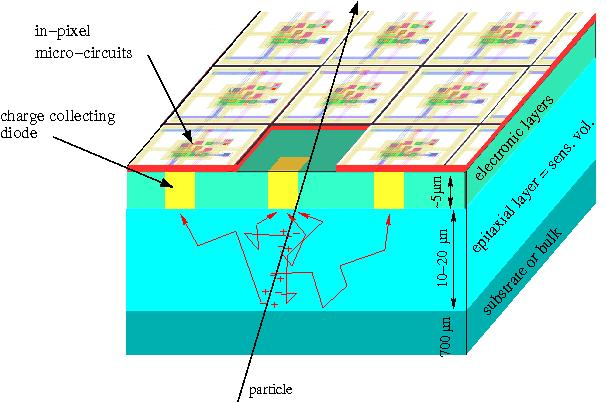
\includegraphics[width = 10cm]{Pictures/vxd/principeMapsMIP.jpg}
      \caption{Drawing of MAPS structure representing the different layers of the sensor and the path of charge carriers in the epitaxial layer.}
      \label{fig:principleMaps}
    \end{figure}

    \subsection{Pros and cons of the technology}

    The \gls{CMOS} sensors have several interesting properties.
    First of all, the fabrication cost is lower than other pixel technologies due to the industrial processes used to build the sensors.
    Therefore, many prototypes and bigger matrices can be built, while benefiting from the industrial experience.
    For example, the imaging industry has developed smaller and smaller grid size and a pitch size of ten microns can be achieved.
    
    Secondly, due to the size of the depleted area, the charge carriers tend to spread more over neighboring pixels.
    On the one hand, the signal collected per pixel is smaller, but on the other hand, the reconstruction of the hit position with a centre of gravity algorithm is improving the spatial resolution.
    To give an idea, a binary output sensor with a pitch of 18.4 $\mu\text{m}$ can achieve a spatial resolution better than 3 $\mu\text{m}$.

    Thirdly, the distinct doping of the different layers is responsible for the reflection of the charge carriers to the collection diodes.
    However, only the interface between two different doped regions is responsible for this reflection.
    Thus, the substrate can be thinned down to few microns leading to a sensor with a thickness of 50 $\mu\text{m}$, while keeping the possibility to manipulate them.
    In this way, the material budget can be reduced down to 0.053\% $X_0$.
    %The bulk is not entirely responsible for the charge carriers reflection, only the interface between the substrate and the epitaxial layer is mainly responsible for the reflection.
    %The substrate can be thinned down to few microns leading to a sensor with a thickness of 50 $\mu\text{m}$ while keeping the possibility to manipulate them.
    %The material budget can then be reduced to 0.053 \%.

    Nevertheless, the thickness of the epitaxial layer (usually between 10 and 15$\mu$m) and the small depleted region are responsible for a small charge collection.
    As a matter of fact, a \gls{MIP} is creating 80 electron/hole pairs per microns, so the number of charges collecting by the diode is of the order of a thousand electrons.
    Hence, the signal created is only a few millivolts and low noise electronics have to be used for processing the signal.

    CMOS sensors are sensitive to ionizing and non-ionizing radiations that degrade the sensor properties.
    The non-ionizing radiations are damaging the crystal structure of the epitaxial layers, creating defaults in the lattice.
    The recombination rate is increasing and reduces the signal collected.
    To avoid this effect, two solutions are possible.
    The first one is to reduce the size of the pixels in order to decrease the path of the particles from the epitaxial layer to the collection diodes.
    Nevertheless, the cost to build sensors with a smaller pitch is increasing.
    The second solution is to increase the resistivity of the epitaxial layer to expand the depleted area.
    
    The ionizing radiations are responsible for charges accumulation in the electronic layer.
    The leakage current is increasing in the pixel and diode collection.
    To reduce the leakage current, smaller diodes can be used to reduce the impact of the leakage current but as it was explained before, the cost of fabrication is increasing.
    
    \subsection{Signal processing}

    If no charge is collected by the pixel, the voltage at the equivalent capacitor of the diode is evolving because of the leakage current inherent in the junction.
    The pixel reading can be done in two different ways, depending on the method used to minimise the leakage current effect.
    Currently, two pixel's architectures are used to compensate the diode's leakage current: the \textit{3 Transistors pixel design}, mainly used in imaging, and the \textit{self-biased pixel design}.
    The circuit diagram which is shown on the figure~\ref{fig:elecArch} represents the two methods to design pixel.

    The first one, presented on figure~\ref{fig:3T}, consists to reinitialise the collection diode's voltage to a reference voltage thanks to a \textit{reset} transistor, denoted M1 on the diagram.
    This method works in two steps. 
    Firstly, the M1 transistor is closed and the charge of the equivalent capacitor $C_d$ associated to the junction P-N, represented by a diode on the diagram, is slowly decreasing because of the diode's leakage current. 
    During this phase, the pixel is sensitive and is read.
    After a time interval equivalent to the integration time of the sensor, the transistor M1 is opened to recharge $C_d$ to its initial voltage.
    During this time, the pixel is not sensitive.
    While M1 is used for the reset, M2 is used as a pre-amplifier of the signal created by the diode and M3 link up the voltage to the output of the circuit.
    Although this compensation method is fast, it generates a dead time for detection between two readings.
    
   % The first method consists to force time to time the reinitialisation of the voltage on the collection diode leads to a reference value thanks to a \textit{reset} transistor.
   % In order to limit the impact of the noise created by thermal fluctuations during the reinitialisation, a \textit{correlated double sampling} is used. A first voltage reading from the output of the pixel stores the \textit{reset} level and a second reading subtracts the measured voltage previously read to reduce the noise impact.
   % Although the compensation is fast, it generates a dead time for detection between two readings.
    
    The figure~\ref{fig:selfBiased} depicts the \textit{self-biased pixel design} method\cite{Deveaux2009}.
    It is using a P-N junction (symbolised here by a diode mounted on the other side) coupled to the N-well implant to absorb the leakage current.
    The inverted diode is continuously compensated the diode's leakage current, thus the dead time vanishes.
    %Using a forward p-n junction has the advantage to avoid any dead-time because the diode's leakage current is continuously compensated by the second diode.
    While no particle is crossing the sensor, an equilibrium appears between the leakage and recharge current.
    A particle going through the sensor disrupts this equilibrium.
    The charges collected by the pixel lead to a discharge of the diode's capacitor $C_d$, followed by a recharge of this capacitor thanks to the second diode to reach again the equilibrium.
    %When a particle is crossing the sensor, the charges are collected by the pixel, leading to a discharge of the diode's capacitor $C_d$, which is followed by a recharge to reach again the equilibrium.
    Nevertheless, if the recharge procedure is too fast compare to the integration time, the physics signal is masked and the passage of the particle is never notified.
    %Nevertheless, the recharge procedure should be slower than the integration time to be able to detect physics signal during detection.
    %Indeed, when the recharge is too fast, the physics signal is masked and the passage of particle will never be notified.
    Even if the time interval to recharge the capacitor $C_d$ is set properly, an important charge collection per pixel could disturb the recharge phase and the pixel will reach a stable level again only a long time interval of the order of 10 ms.

    \begin{figure}[!h]
    \centering
    \begin{subfigure}[t]{0.45\textwidth}
        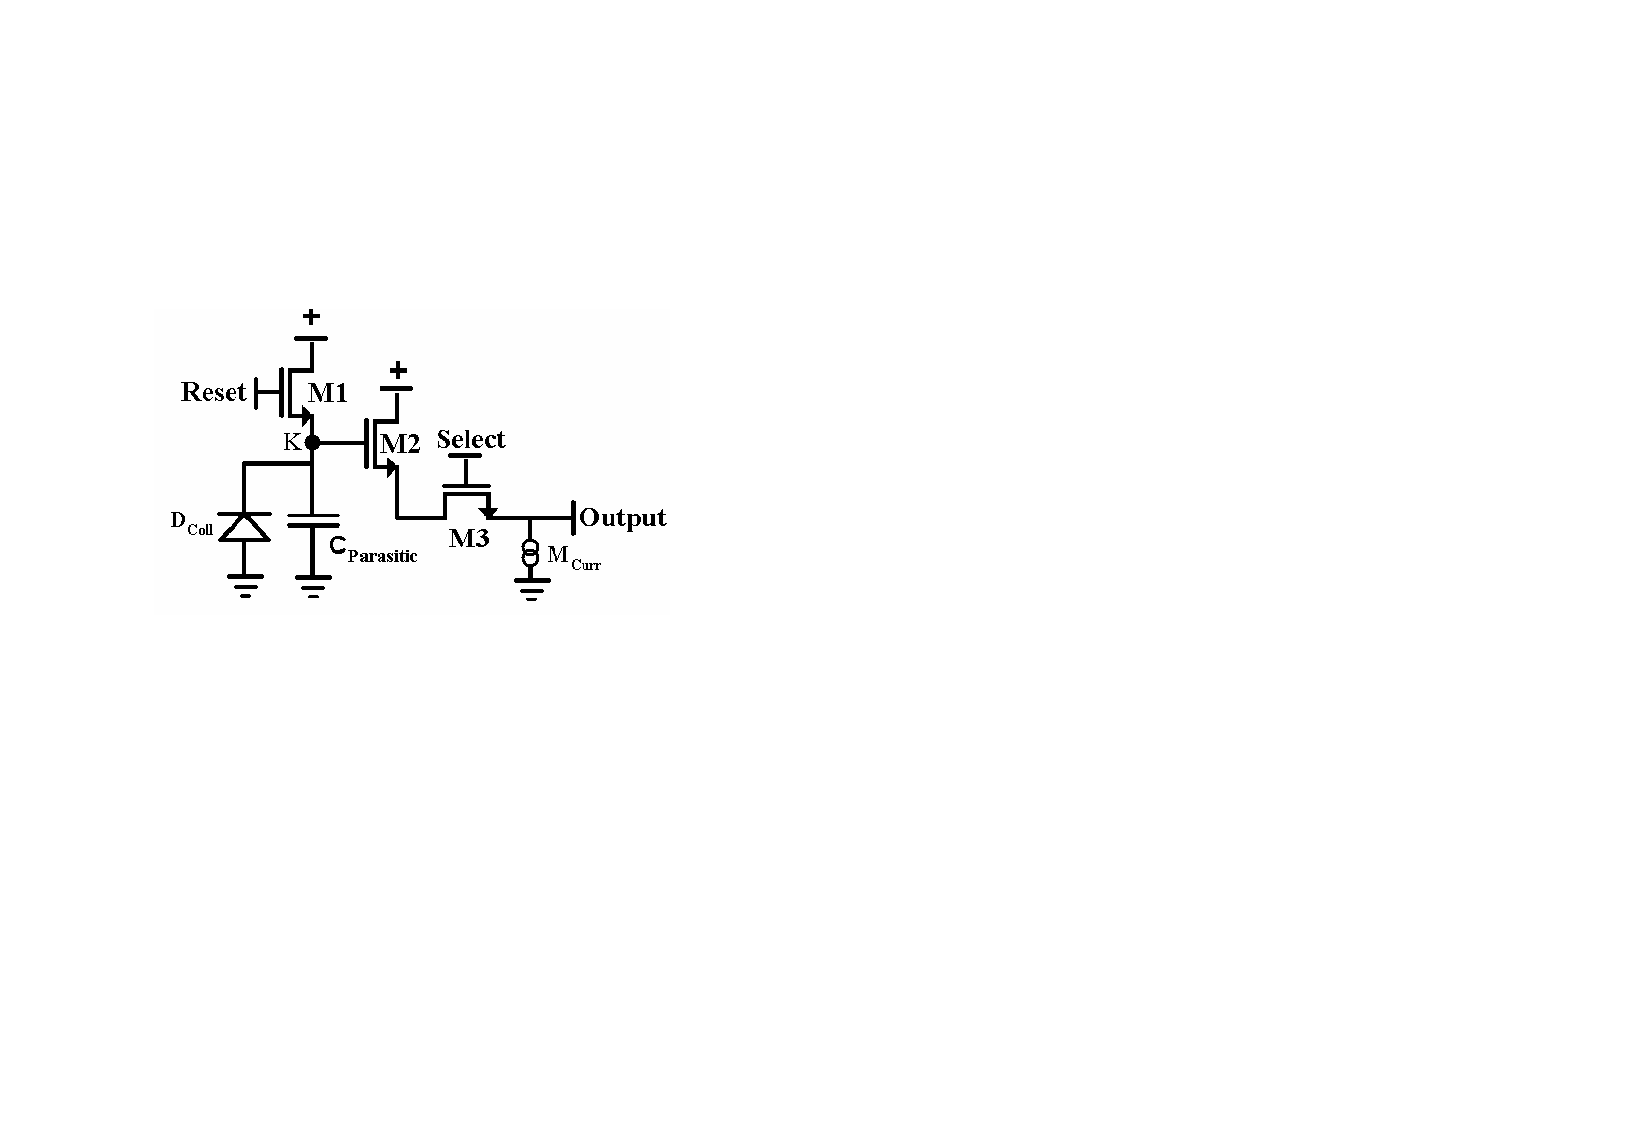
\includegraphics[width=\textwidth]{Pictures/vxd/3T_architecture.pdf}
        \caption{Three transistors (3T) pixel design.}
        \label{fig:3T}
    \end{subfigure}
    ~%\quad
     %add desired spacing between images, e. g. ~, \quad, \qquad, \hfill etc. 
      %(or a blank line to force the subfigure onto a new line)
    \begin{subfigure}[t]{0.45\textwidth}
        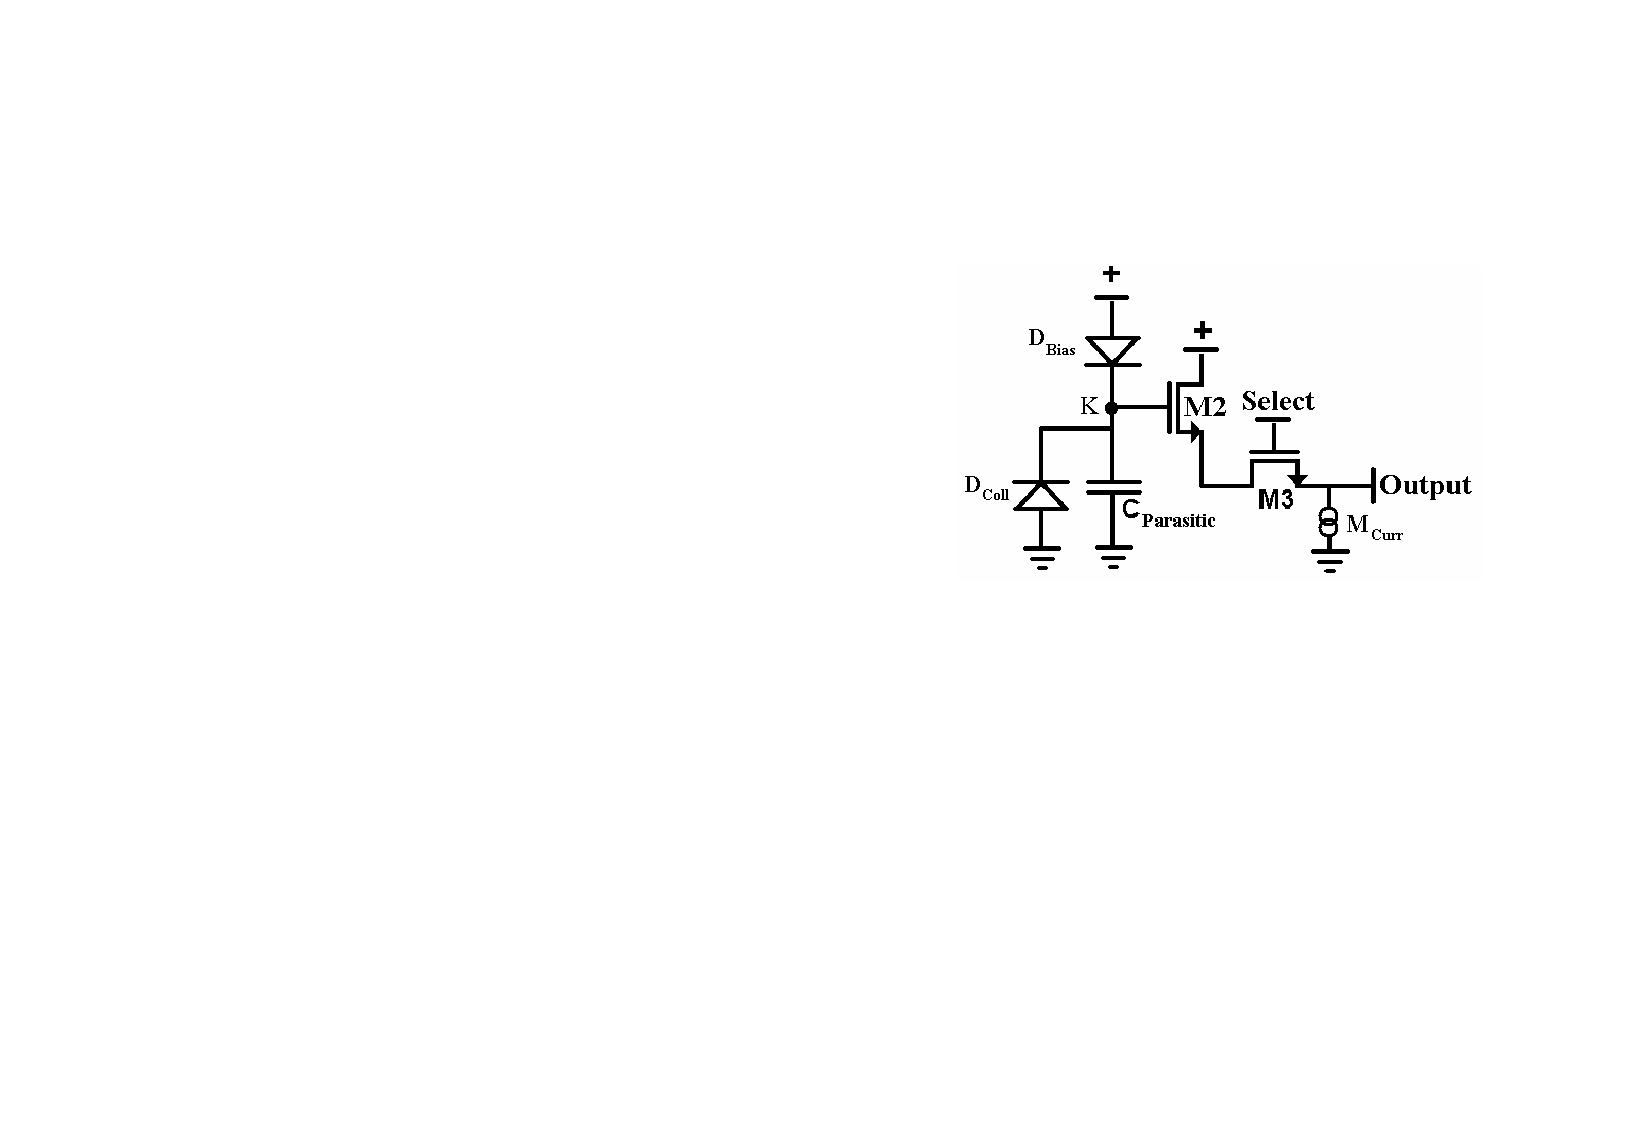
\includegraphics[width=0.95\textwidth]{Pictures/vxd/self-biased_architecture.pdf}
        \caption{Self-biased pixel design.}
        \label{fig:selfBiased}
    \end{subfigure}
      \caption{Two different architectures of pixel.}
      \label{fig:elecArch}
    \end{figure}    

    \subsubsection{Integration time and readout}

    For a non-depleted epitaxial layer, the charge carriers are thermally diffused to the collection diodes.
    The time to collect these charges in a pixel is $\sim$ 100 ns, setting a maximal limit to read the signal.
    This integration time is not reachable due to other factors, like the pixel occupancy or the time needed to obtain the information of all the pixels.
    Also, a compromise to reach fast integration time has to be done.
    Faster is the sensor, more important is the power consumption of the electronic.
    Moreover, to reduce the integration time, a solution consists of increasing the size of the pixels.
    In consequence, the pointing resolution of the device is impacted.
    For the case of the \gls{ILC}, the integration time is dictated by the pixel occupancy that should not be bigger than a percent, to stay in the using sensor's range and to be able to reconstruct the impact.

    The first sensors developed were using an analog output.
    With this approach, the pixels were addressed sequentially and their output was multiplexing in one bus line.
    The advantage of such method is that the discrimination can be adjusted offline for each pixel, thus compensating the nonuniform response.
    Nevertheless, the integration time is depending on the operational frequency of the bus (usually 50 MHz) and the number of pixels contained in a matrix.
    For a sensor having millions of pixels, the integration time is then of the order of the millisecond.
    An analog output is then too slow for a \gls{ILC} purpose. 
    
    \begin{figure}[!h]
      \centering
      \missingfigure{Rolling shutter}
      \caption{Parallel column readout.}
      \label{fig:rollShut}
    \end{figure}
    
    To overcome this problem, an approach is to group the pixels in columns and to read them in parallel.
    The figure~\ref{fig:rollShut} depicts the principle of this method called \textit{column parallel readout} or \textit{rolling-shutter}.
    Instead of having one bus line for the whole matrix, each column has its own bus and a data sparsification logic is integrated on the periphery of the sensor.
    One row is read out between 100 ns and 200 ns, independently to the number of pixels contained in it.
    In consequence, a matrix containing thousands of rows has an integration time of $\mathcal{O}(100\mu$s).
    Moreover, to increase the integration time an output memory is duplicated at the periphery of the sensor.
    Hence, when one line is read, the precedent one is processed by the electronics at the end of each bus line of each column.
    To minimise the data bandwidth, only the pixels above certain thresholds are read thanks to discriminators coupling to a zero suppression logic, called \gls{SUZE}.
    In this way, only the address of the first pixel hit in a row and the number of the adjacent fired ones are stored.
    This memory is duplicated to be able to process one row, while the previous one is read out by the outside world.
    In order to increase the readout speed, two techniques are conceivable\cite{Winter:2009zz}.
    The first one provides elongated pixels in the vertical direction in order to reduce the number of rows, thus degrading the spatial resolution in the same direction.
    The second one consists of dividing the columns into two distinct parts, which have its dedicated output.

    %When one line is read, the precedent line is processed by the electronics on the bottom each column.
    %Only the pixels having a signal above certain thresholds are read.
    %A zero suppression logic, called \gls{SUZE}, is in charge to determine the number of fired pixels in a raw and to send the address of the first pixel hit and the number of adjacent ones hit, as shown on figure~\ref{fig:SUZE}.
    %The sequence of fired pixels feed one output memory, while a second memory is read out by the outside world.
    %This technique has the advantage to reduce the data bandwidth.
    %The integration time is then defined as the time to read one line by the number of rows in the matrix.
    %For example, sensors containing a thousand of lines have an integration time of $\mathcal{O}(100\mu$s). 
    %Two techniques can be used to increase the readout speed\cite{Winter:2009zz}.
    %The first one provides elongated pixels in the vertical direction in order to reduce the number of rows, thus degrading the spatial resolution in the same direction.
    %The second one consists of dividing the columns into two distinct parts, which have its dedicated output.

    \begin{figure}[!h]
      \centering
      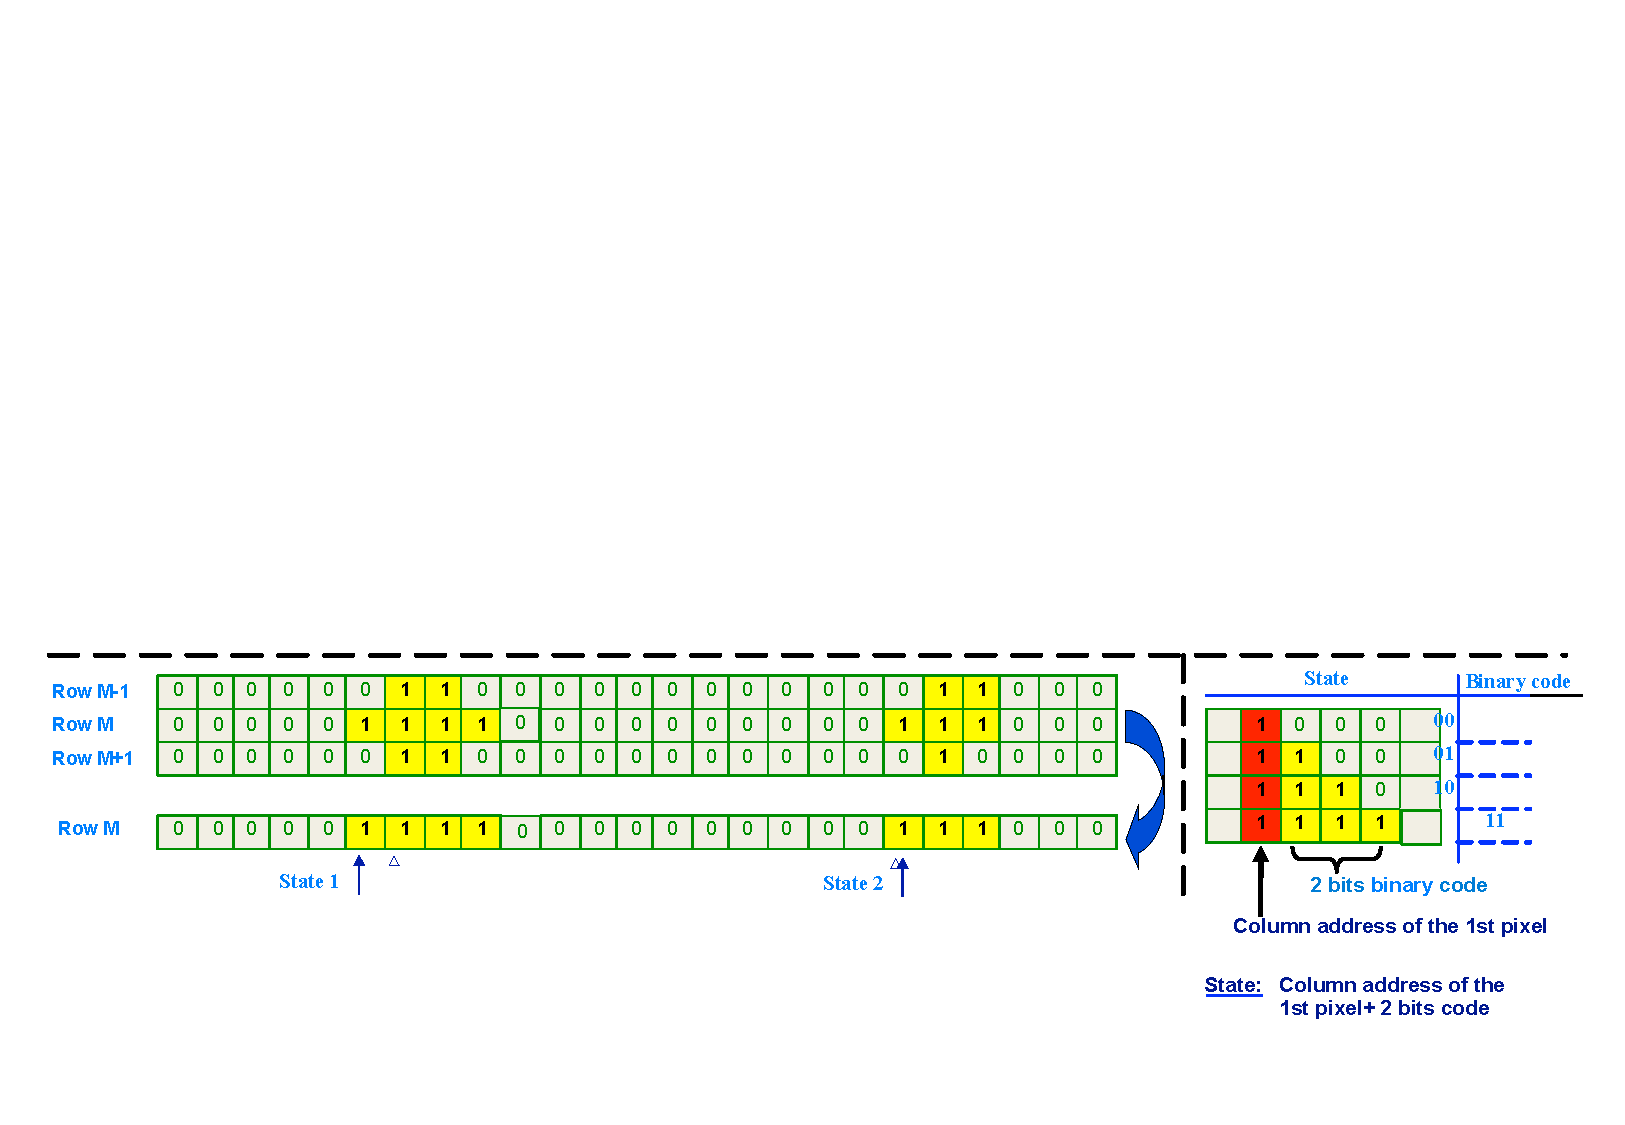
\includegraphics[width=\textwidth]{Pictures/vxd/suze_hit.pdf}
      \caption{Principle of the zero suppression logic. }
      \label{fig:SUZE}
    \end{figure}

    \subsubsection{Noise}

    The \gls{CMOS} sensors are sensitive to the noise.
    Many factors are causing it and the different kind of noise is divided into two categories: the \gls{FPN} and the \gls{TN}.
    The non-uniformity responses of the pixel in a sub-array is responsible for the \gls{FPN} and is regarded as an offset or pedestal, which is subtracted from the pixel response to reduce the impact of this noise.
    The \gls{TN} has different origins, as the shot noise, the pink noise or the thermal noise.
    The different operational phases to read the signal are contributing to the noise.
    
    One contribution to the \gls{TN} appears in the \textit{3T pixel design} only during the reset phase.
    This noise arises when the transistor is open restoring the charge of the capacitor associated with the collection diode.
    It is dependent on the temperature and the diode's capacitance.
    
    The second one is the noise during integration and is caused by statistical fluctuations of the leakage current (shot noise).
    Faster is the integration time, slower is the shot noise contribution.
    
    Finally, the third one arises from the readout, while the column switch and the source follower capacitors are working.
    This noise depends on the contribution of each capacitor.
    
    To remove the \gls{FPN} and the reset noise, a \gls{CDS} is performed inside the pixel or at the bottom of the column.
    It consists to acquire two frames and to subtract the first one to the second one to search for possible signals.
    The chapter~\ref{chap:labTests} describes the steps to characterise the \gls{FPN} and \gls{TN} and to select an appropriate \gls{SNR} in order to minimise the noise contribution, and to find a range on which the sensor is working properly.


    \subsection{State of the art in high energy physics}
    \label{subsec:Mi26}

    \begin{figure}
      \centering
      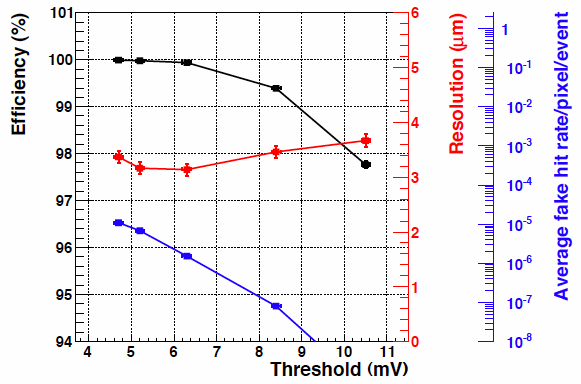
\includegraphics[width=0.8\textwidth]{Pictures/vxd/MIMOSA26_chip26_HR15_20deg}
      \caption{Plots representing the efficiency, the fake hit rate per pixel and the spatial resolution as a function of the discriminator threshold.}
      \label{fig:mi26Perf}
    \end{figure}

    The first full-scale digital sensor developed by the PICSEL group was the \gls{MIMOSA}-26.
    They were designed to equip the reference planes of the EUDET beam telescope and are used since 2010 to build the PLUME prototypes.
    It is fabricated in the AMS $0.35\mu\text{m}$ technology, and has a matrix containing approximately $6.6 \times 10^5$ pixels, distributed in 1152 columns and 576 rows.
    The pixel pitch is $18.4\mu\text{m}$ and the sensitive area represents $21.2 \times 10.6 \text{cm}^2$.
    The readout of the matrix is ensured by a rolling-shutter working at 80MHz frequency, hence the integration time is $115.2\mu\text{s}$.
    The signal produces by the charge collection inside the pixel is firstly amplified.
    Then, the \gls{CDS} technique is used to subtract successive frames before to send the signal at the bottom of the pixel array, where the signal processing circuitry is placed.
    Analog to digital conversion is done, coupled to a second double sampling, in order to reduce the \gls{FPN}.
    The output of the discriminators is then connected to a zero suppression logic, in which an output memory is duplicated to ensure a continuous readout.
    The signal is finally transmitted to the outside world.
    The architecture of the \gls{MIMOSA}-26 is represented by a block-diagram on figure~\ref{fig:archMi26}.
    The power consumption is $1.1\mu\text{W/pixel}$ and the sensor is thinned down to $50\mu\text{m}$ in order to minimise the multiple scattering inside the volume.
    The performances obtained with a \gls{MIMOSA}-26 are shown on the figure~\ref{fig:mi26Perf}.

  \begin{figure}[!h]
    \hspace{-2cm}
    \centering
    \begin{subfigure}[t]{0.4\textwidth}
        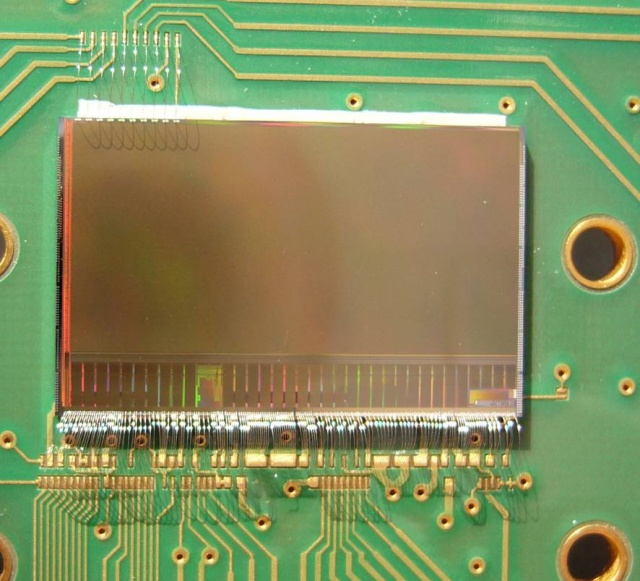
\includegraphics[width=0.95\textwidth]{Pictures/vxd/mi26.jpg}
        \caption{Picture of a MIMOSA-26 mounted on a PCB.}
        \label{fig:mi26}
    \end{subfigure}
    \qquad
     %add desired spacing between images, e. g. ~, \quad, \qquad, \hfill etc. 
      %(or a blank line to force the subfigure onto a new line)
    \begin{subfigure}[t]{0.4\textwidth}
        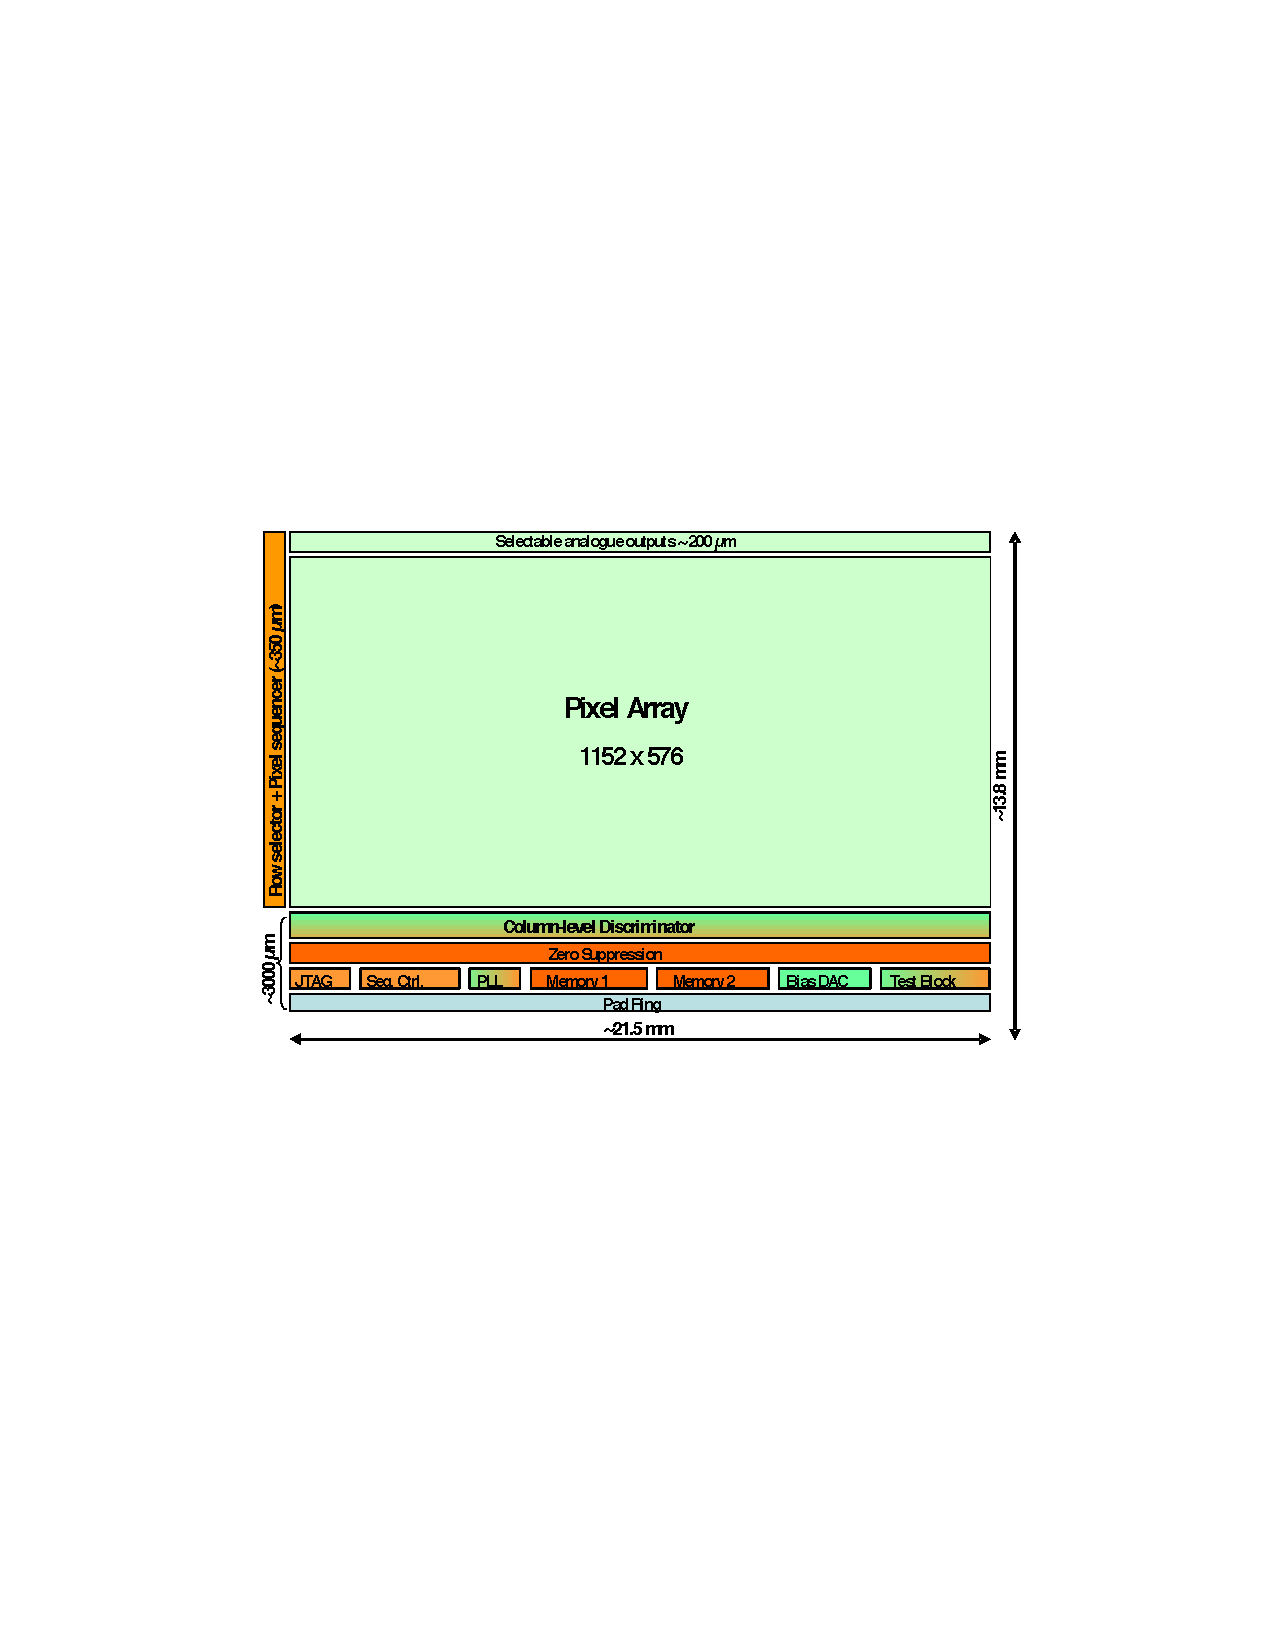
\includegraphics[width=1.35\textwidth]{Pictures/vxd/mi26_architecture.pdf}
        \caption{Layout of the MIMOSA-26 matrix.}
        \label{fig:archMi26}
    \end{subfigure}
    \caption{Block-diagram and a picture of the MIMOSA-26}\label{fig:Mi26}
    \end{figure}    



    The PICSEL group has then developed digital output sensors for the pixel vertex detector at the START experiment at Brookhaven National Laboratory\cite{}.
    The figure~\ref{fig:Mi28} is showing a half-section of the STAR vertex detector (subfigure~\ref{fig:vxdSTAR}) and a \gls{MIMOSA}-28 bounded on a PCB(subfigure~\ref{fig:ultimate}).
    They are based on the architecture of \gls{MIMOSA}-26 with some modifications.
    The matrix contains 960 columns and 928 rows for a pitch of $20.7 \times 20.7 \mu\text{m}^2$.
    The sensitive area is 19.7 x 19.2 $\text{cm}^2$, for an integration time of less than $200\mu\text{s}$.
    The sensor can reach a particle detection rate of $10^6$ particles/$\text{cm}^2$/s. 
    Finally, their power consumption is lower or equal to 150 mW/$\text{cm}^2$.
    The spatial resolution obtained for ULTIMATE is less than 4 $\mu\text{m}$.

  

    %The PICSEL group has developed sensors, called ULTIMATE, for the STAR experiment at Brookhaven National Laboratory\todo{REF to a paper}.
    %They are based on \gls{MIMOSA}-28 sensors and are integrated into the vertex detector.
    %The choice for this technology was made because of their characteristics.
    %Indeed, the thickness of a sensor is around 50 $\mu\text{m}$ in order to minimise the multiple scattering of particles.
    %The matrix is made of roughly $9 \times 10^5$ pixels, corresponding to 960 columns and 928 rows for a pitch of 20.7 x 20.7 $\mu\text{m}^2$.
    %The sensitive area is 19.7 x 19.2 $\text{cm}^2$.
    %They have a binary output integrating a zero suppression technology (SUZE) and the integration time of the whole matrix is 200 $\mu\text{s}$.
    %Thanks to this architecture, the sensors can reach a particle detection rate of $10^6$ particles/$\text{cm}^2$/s. 
    %Finally, their power consumption is lower or equal to 150 mW/$\text{cm}^2$.
    %The spatial resolution obtained for ULTIMATE is less than 4 $\mu\text{m}$.

  \begin{figure}[!h]
    \centering
    \begin{subfigure}[t]{0.4\textwidth}
        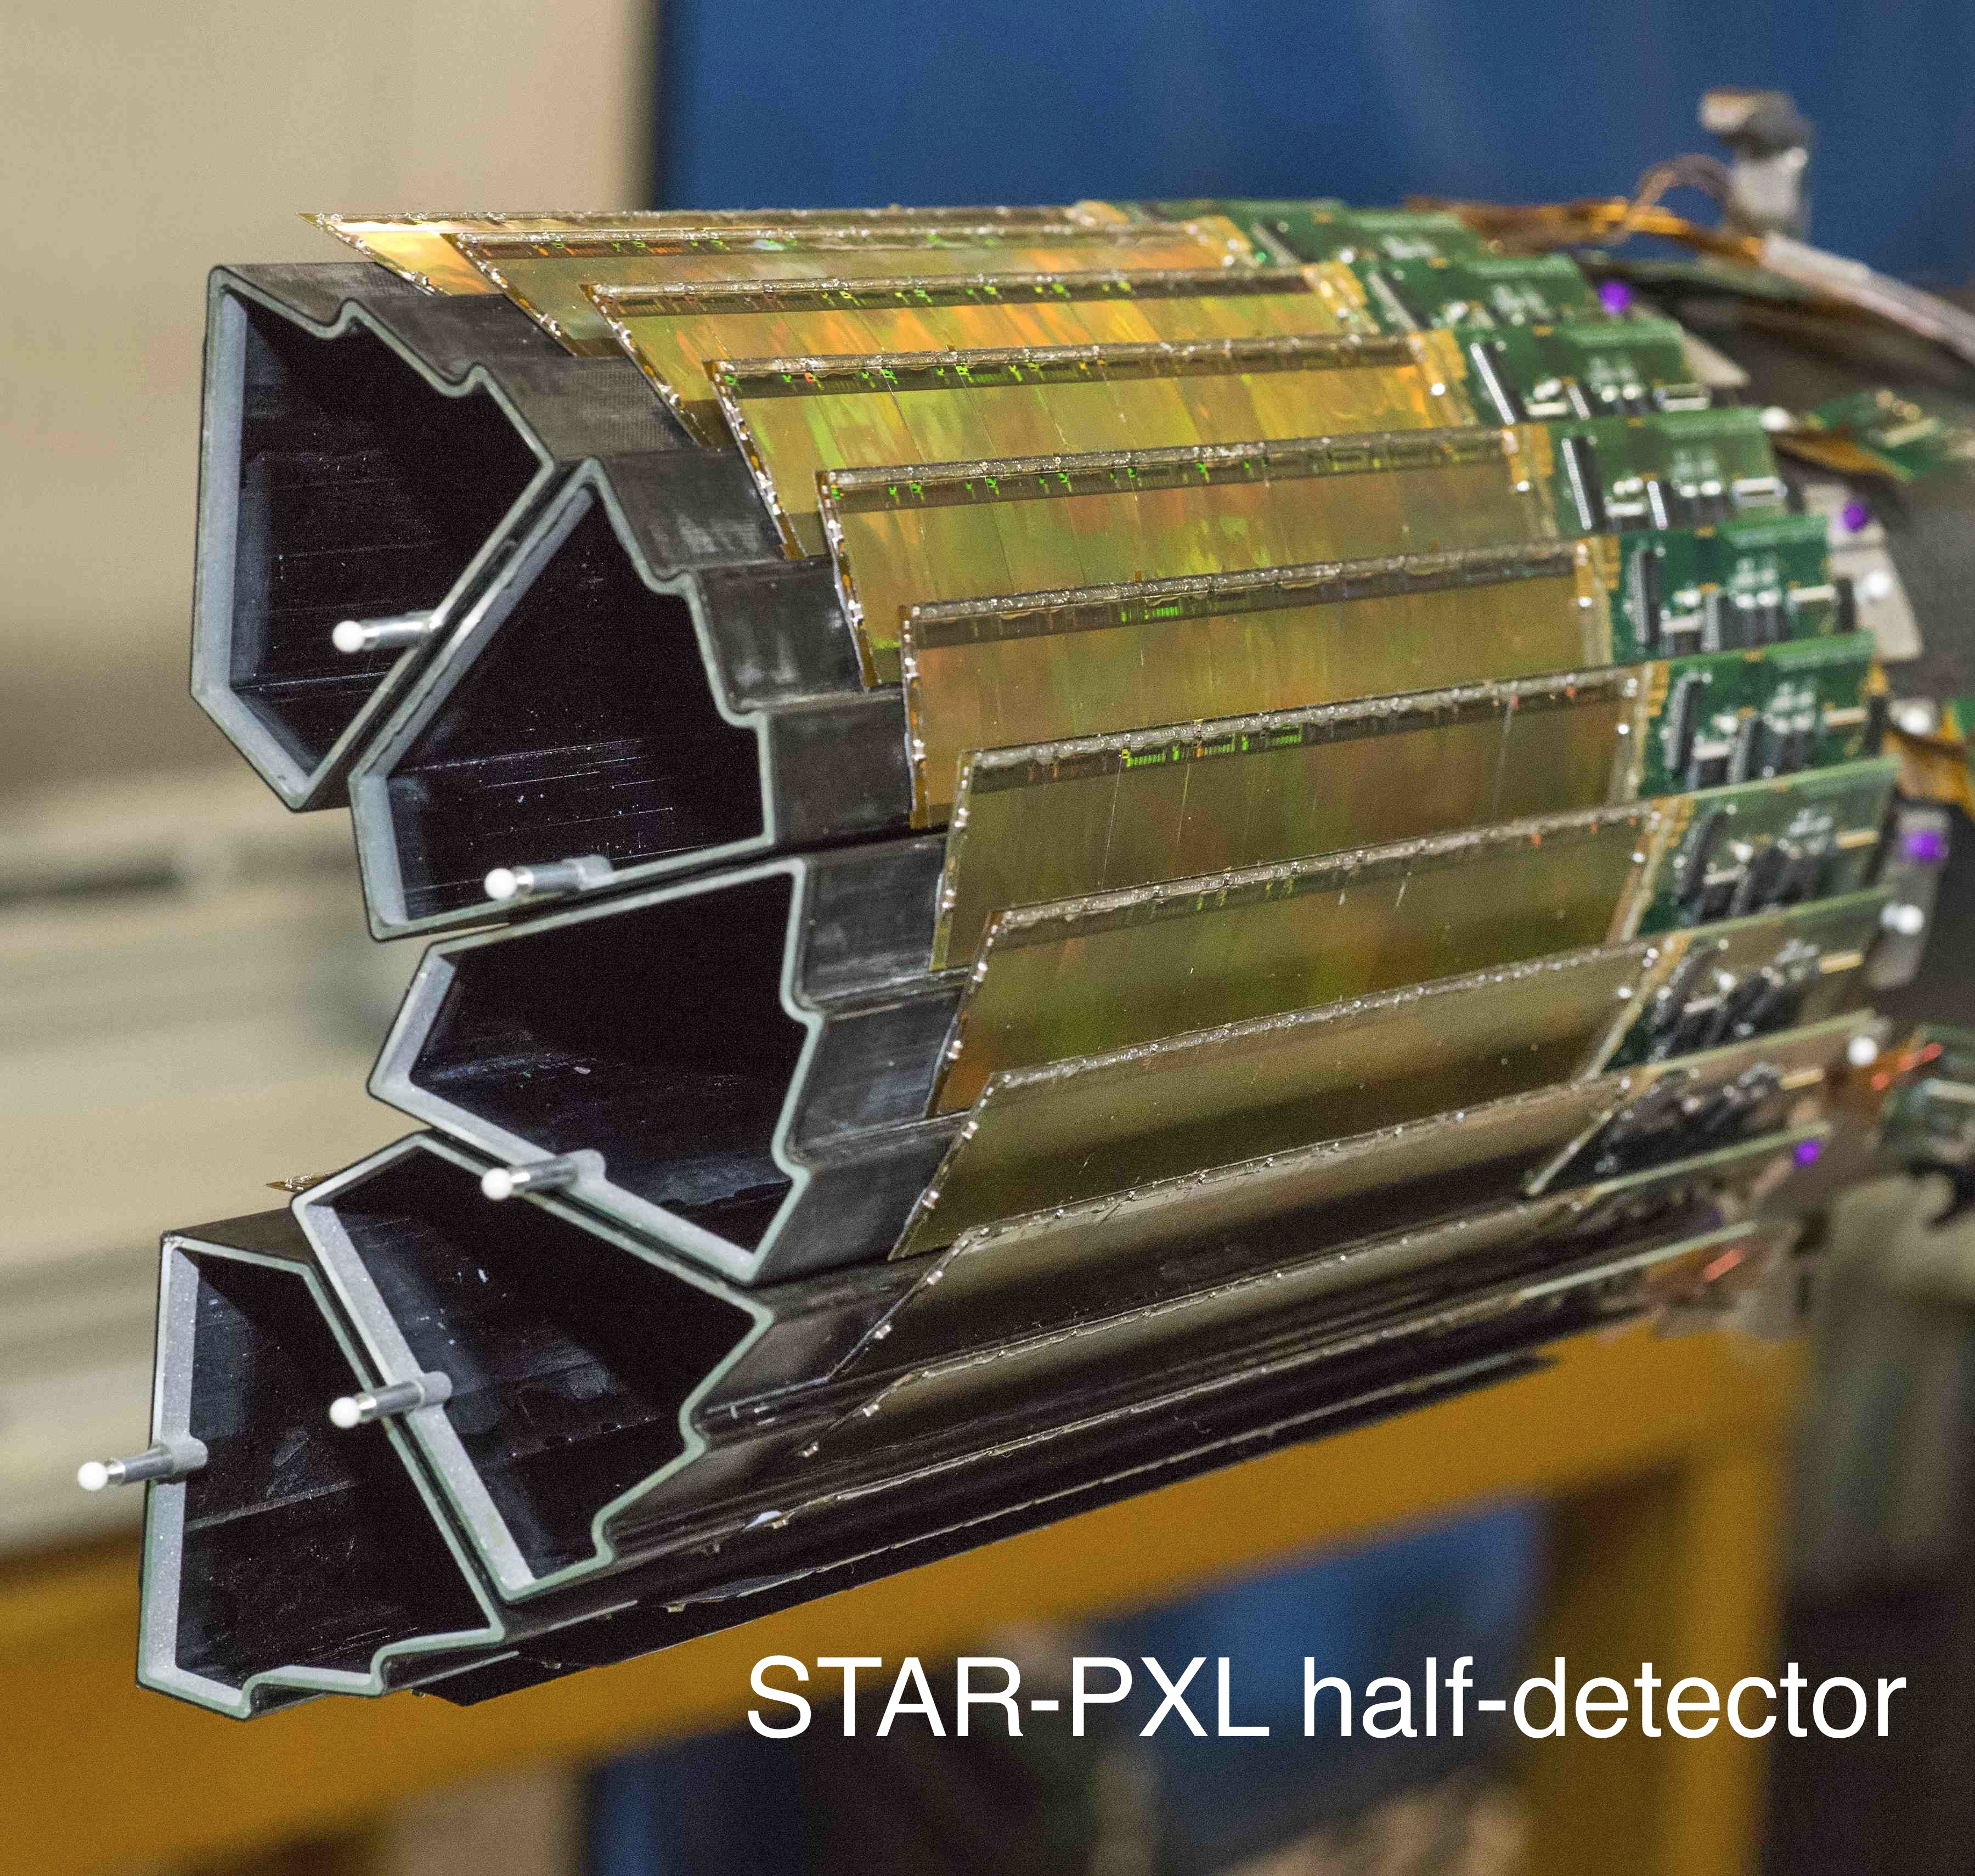
\includegraphics[width=\textwidth]{Pictures/vxd/pxlFinal_sideView_smallSize.jpg}
        \caption{Half part picture of the pixel vertex detector at STAR.}
        \label{fig:vxdSTAR}
    \end{subfigure}
    \qquad
     %add desired spacing between images, e. g. ~, \quad, \qquad, \hfill etc. 
      %(or a blank line to force the subfigure onto a new line)
    \begin{subfigure}[t]{0.4\textwidth}
        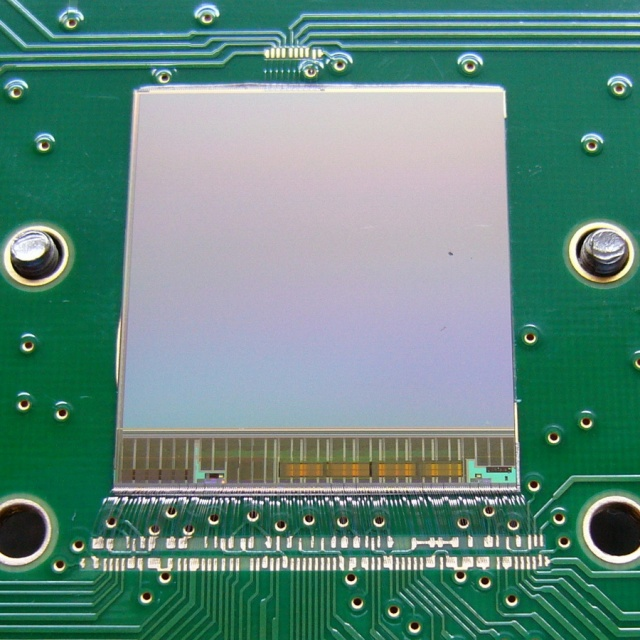
\includegraphics[width=0.95\textwidth]{Pictures/vxd/ultimate2.jpg}
        \caption{ULTIMATE chip mounted on a PCB. %The top wire bounds are used for a slow analog output dedicated to lab test, while the bottom ones are the wire bounds which control and read the sensor. }
        }
        \label{fig:ultimate}
    \end{subfigure}
    \caption{Pictures of the STAR vertex detector and an ULTIMATE chip}\label{fig:Mi28}
    \end{figure}    


    This chapter has depicted the purpose of the vertex detector for the \gls{ILD}.
    Different technologies were introduced, to focus specifically on the \gls{CMOS} sensors and their use in high-energy physics.
    The \gls{PLUME} collaboration aims to integrate \gls{MAPS} onto light double-sided ladders, in order to reach the requirements of the \gls{ILC}.
    The collaboration has reach different steps to produce the first full-scale ladder, which have only a material budget of only $0.35\% X_0$ and a spatial resolution better than $4\mu\text{m}$.
    The principle of the \gls{CMOS} technology was presented. 
    The next chapter is focusing on the electrical validation of this sensors mounted onto a PLUME ladder.

    




    %\chapter{PLUME laboratory testing}
\chapter{Basic assessments}
\label{chap:labTests}

  In chapter~\ref{chap:vxd}, an overview of the \gls{PLUME} project was presented.
  Since 2010, the collaboration is building full-scale and fully functional ladders and is trying to reduce the material budget down to $0.35~\%$ of $\rm{X_{0}}$.
  Due to the six sensors working together and the huge amount of electrical lines to control and read the different sensors on a module, these ladders have to be carefully tested and validated in the laboratory before performing tests under real conditions at \gls{CERN} or \gls{DESY} test beam facilities.
  This chapter introduces the different steps from the assembly procedure performed at Strasbourg (for the module) and Bristol (for a complete ladder), to the final tests to study the sensor's responses including electrical functionality tests at Hamburg.
 
 \minitoc
  
  %\begin{itemize}
  %  \item Describe bench
  %  \item Describe control of a sensor
  %  \item Describe output of Mi-26
  %\end{itemize}

\section{PLUME assembly procedures}

  The ladders are built in two steps. 
  Two independent modules are assembled at Strasbourg and then tested at \gls{DESY}. 
  These modules consist of a flex-cable on which \gls{MIMOSA}-26 sensors are glued.
  Afterwards, they are shipped to Bristol where the modules are glued together on a \gls{SiC} foam to form a \gls{PLUME} ladder.
  The assembly procedures are introduced below, as well as the visual inspection between the mounting steps.

  \subsection{Module and ladder assembly}

    \subsubsection{Module assembly}
    \label{subsec:modAssembly}

    The module assembly is performed at the \gls{IPHC} by the microelectronics group and is done in three steps.
    First of all, passive components (capacitors, resistors) are soldered onto a flex-cable.
    To reinforce the flex-cable around the connector area, an epoxy layer with a thickness of $300~\rm{\mu m}$ is applied on the flex-cable's back-side.
    This layer is limited only to the connector area, increasing locally the material budget.
    

  %  Then, an epoxy layer with a thickness of $300~\rm{\mu m}$ is applied on the back side of the flex-cable, in the connector area.
   % Due to the force applied by pulling and pushing the jumper cable on the \gls{ZIF} connector, the epoxy layer is used to reinforce this area and to avoid damaging the flex-cable.
    Secondly, the module is then placed on a metal jig to ensure its flatness using a vacuum suction.
    The next step is to glue the six sensors onto the flex.
    The positioning of the chips used to be done manually, but a programmable robot, which has a maximum mismatch alignment reaching approximately $20~\mu\rm{m}$, is now used for this procedure.
    As the sensors are thin and fragile, they are manipulated with a vacuum sucker.
    A few drops of glue are dispensed on the flex and then, these sensors are gently pressed one by one on top of it to be glued.
    Afterwards, the glue is cured in an oven. After this step, the chips cannot be removed anymore.
    If a sensor is not working properly, it can not be replaced by a new one because the force needed to remove it might break the fragile flex-cable.
    In the worse case scenario, a new sensor can be glued on top of it, but this solution cannot be envisaged for a real ladder as it increases locally the material budget.
    To avoid this situation, a sensor probe-test is performed to select only good sensors before the module assembly.
    This step is done at the IK in Frankfurt.
    The final step consists of soldering the 540 wire-bonds (a single \gls{MIMOSA}-26 requires 90 wire-bonds) using a semi-automatic machine.
    Wire-bonds can be protected by applying a glob-top epoxy~\cite{minges1989electronic}.
    It has the advantage of offering protection against moisture or contaminants, adding electrical insulation and prohibiting their movement during other manipulations (see section~\ref{subsec:visualInspection} for the utility of the glob-top epoxy). 
    Nevertheless, it increases locally the material budget and if an electrical problem occurs, the wire-bonds cannot be disconnected.
    Once the module is assembled, it is finally transferred onto a plastic sole, which has alignment pins.
    This sole helps with the manipulation of a module, but also reduces the stress on the flex-cable, by holding it as flat as possible.
    During shipping, a plastic cover is screwed on top of this sole to completely protect the module.

    \subsubsection{Ladder assembly}

    The ladder assembly is performed by the Bristol team.     
    The assembly comprises the gluing of two modules on a spacer (\gls{SiC}) and a bate 

    It consists of gluing two modules together on a spacer (\gls{SiC}) and a bate (an aluminum plate).
    The operation is done entirely by hand.
    Each module is placed on a separate jig containing grooves and alignment pins to ensure the positioning, as presented in figure~\ref{fig:ladderAssemblyStep1}.
    The sensitive side of the module is facing the jig to have an access to the rear of the flex-cable for gluing.
    Then, foam is placed on one module below the sensors, while a bate is glued below the connector with an overlap on this foam (see figure~\ref{fig:ladderAssemblyStep2}).
    The second module receives some glue on its backside before the jigs are assembled together.
    Then, glue is cured for one day.
    The amount of glue needed for the assembly was studied carefully. 
    As the foam's surface is irregular, if not enough glue is used, then gluing will not work.
    But if too much glue is used, the jigs might be stuck together.
    When the ladder is finally ready, it is placed into an aluminum box used for testing and shipping.
     
    \begin{figure}[!tbh]
      \centering
      \begin{subfigure}[t]{0.4\textwidth}
          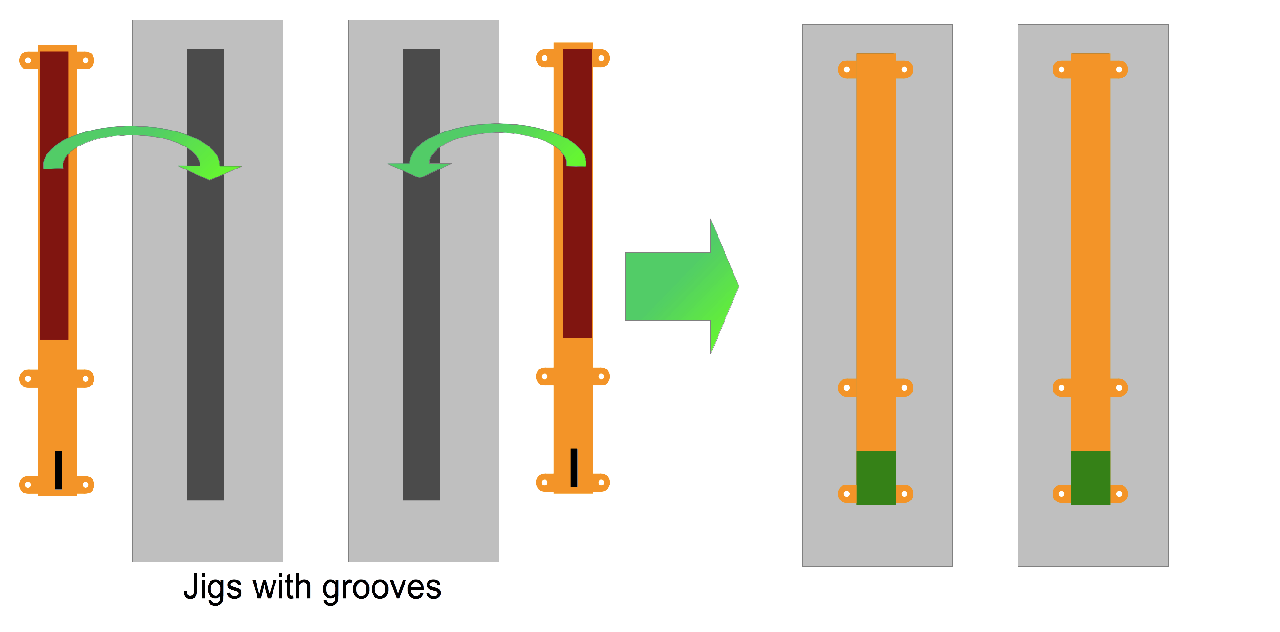
\includegraphics[width = 1.3\textwidth]{Pictures/labTests/plumeLadderAssembly_step1.png}
          \caption{}
          \label{fig:ladderAssemblyStep1}
      \end{subfigure}
      
      %\qquad
       %add desired spacing between images, e. g. ~, \quad, \qquad, \hfill etc. 
        %(or a blank line to force the subfigure onto a new line)
      \begin{subfigure}[t]{0.4\textwidth}
          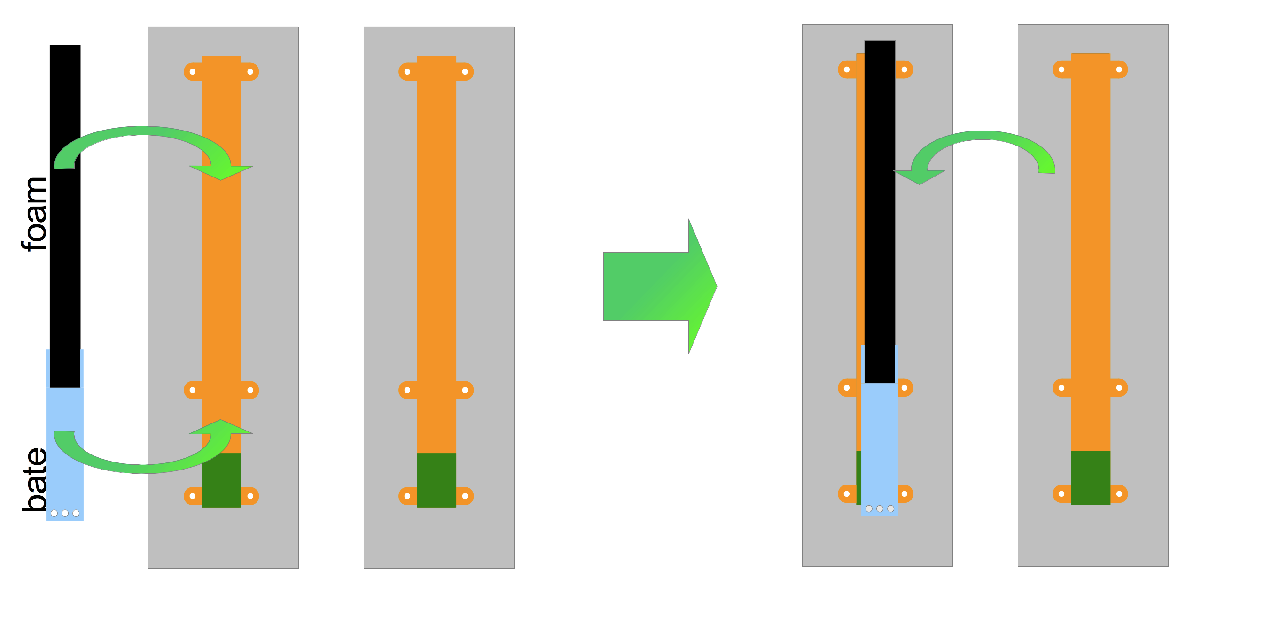
\includegraphics[width = 1.3\textwidth]{Pictures/labTests/plumeLadderAssembly_step2.png}
          \caption{}
          \label{fig:ladderAssemblyStep2}
      \end{subfigure}
      \caption{Drawing of the ladder assembly. The modules are first placed on the jigs, sensors facing the grooves~\ref{fig:ladderAssemblyStep1}, then the foam and the bate are glued between the two modules~\ref{fig:ladderAssemblyStep2}.}
      \label{fig:ladderAssembly}
    \end{figure}    

  \subsection{Visual inspections}
  \label{subsec:visualInspection}

  As explained in section~\ref{subsec:modAssembly}, the sensor positioning was performed first manually and later was switched to an automatic procedure.
  To tune properly the robot which is in charge of gluing the sensors on the flex-cable, the microelectronic group needs a position feedback.
  Each module is then inspected under a microscope to measure the gap between two sensors, and their position relative to each other.
  The distance between the last pixel of a sensor to the first one on the next sensor should be less than $500~\mu\rm{m}$, taking into account the robot's $20~\mu\rm{m}$ mismatch.
  Figure~\ref{fig:visAlign} is a picture taken with a microscope showing the relative position of two sensors on the bottom of the matrix for an aluminum straight module.
  %A visual inspection of the position,  as well as any problem on the matrix, as a crack, as well as a check of the wire-bonds have to be done before any electrical validation.
  The gap between the two edges is $\sim 51~\mu\rm{m}$. 
  
  \begin{figure}[!tbh]
    \centering
    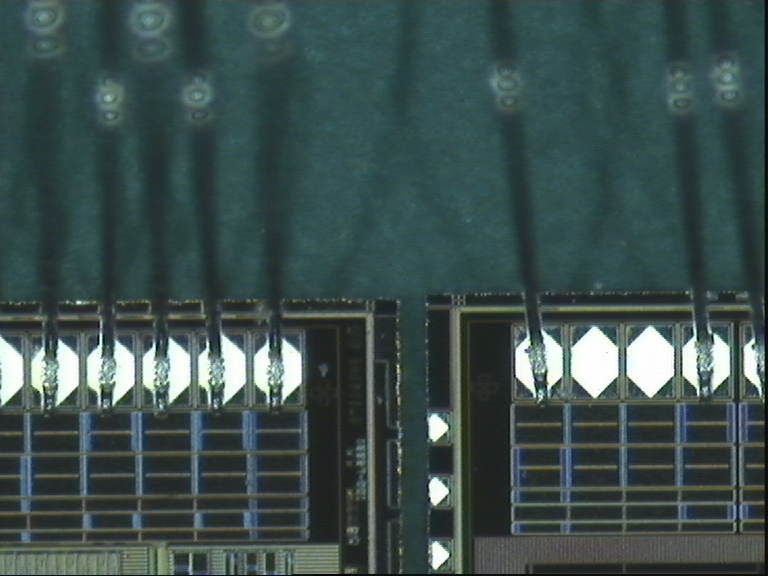
\includegraphics[width=0.6\textwidth]{Pictures/labTests/alignment_sensors.jpg}
    \caption{Visualisation of the alignment. The distance between the two edges is $\sim 51~\mu\rm{m}$.}
    \label{fig:visAlign}
  \end{figure}
  
  A visual inspection is also needed to check if wire-bonds are correctly connected to the right sensor's pad and to verify that the gluing procedure did not break one of the sensors due to some dust.
  Moreover, this inspection is needed to determine if modules were damaged during shipment.
  The modules are fragile objects that have to be manipulated with care.
  Any wrong manipulation can damage severely the vital functionality.
  For example, figure~\ref{fig:wireBondsCrashed} shows a picture taken with a microscope of  wire-bonds crushed by a cable falling.
  Sensitive parts and electronics were not damaged, but some wires were in contact leading to a shortcut.
  Fortunately, the microelectronic group at Strasbourg was able to unbend the wires and repair the most damaged ones.
  This module is now fully operational again and working correctly.
  %By using the glob-top method, the wire-bonds can survive to falling cable, but if they are not assigned to the right pad, there is no possibility to correct it anymore.

  \begin{figure}[!tbh]
    \centering
    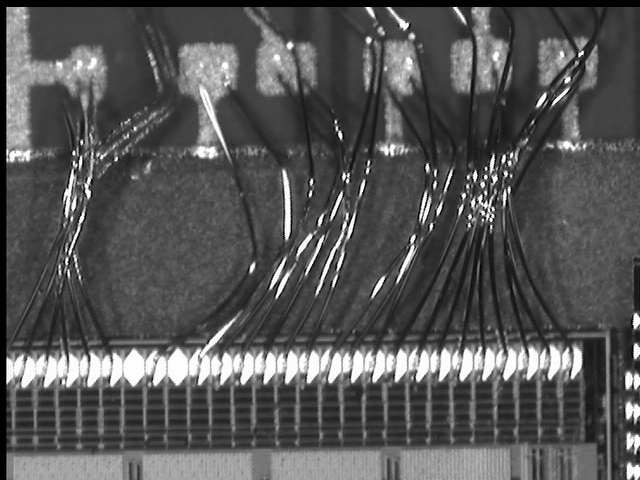
\includegraphics[width=0.6\textwidth]{Pictures/labTests/crash_bonds.jpg}
    \caption{Picture taken with a microscope showing crushed wire-bonds due to a falling cable. Some of the wire-bonds are in contact leading to a shortcut and a non-functional module.}
    \label{fig:wireBondsCrashed}
  \end{figure}

\section{Electrical validation}

  The electrical validation of a \gls{PLUME} module or ladder is performed in two steps.
  The first one consists of checking that all the systems controlling and powering the module are working. 
  Then, a module is connected and its power-consumption, as well as its communication, are checked.

  \subsection{Auxiliary board}

  A module or a PLUME ladder is connected to the outside world by plugging a jumper cable on a \gls{ZIF} connector at one of its edges.
  This jumper cable is linked to an auxiliary board which powers the module's sensors, but also drives them.
  It is also used to transfer the data to the data acquisition system.
  This auxiliary card is connected to a power supply board which provides the nominal voltages needed by the sensors.
  The power supply board delivers the digital and analog voltages ($\rm{V}_{\rm{DD_D}}$ and $\rm{V}_{\rm{DD_A}}$ are set to $3.3~\rm{V}$ using two independent potentiometers), the buffer voltage $\rm{V}_{\rm{CC}}$ fixed to $3.3~\rm{V}$, as well as the voltage for the temperature measurement diodes, a $\pm 5~\rm{V}$ supply for trigger and a power pulsing signal.
  For laboratory testing of a module, the power pulsing option is deactivated by connecting this pin to the $+5~\rm{V}$ pin of the trigger.
  The clamping voltage $\rm{V}_{\rm{clp}}$ used for the polarisation of the pixel has to be in the range $\left[2, 2.2\right]~\rm{V}$.
  On the first version of the auxiliary board, $\rm{V}_{\rm{clp}}$ was provided by an external power supply, but the new version delivers the $2.1~\rm{V}$ needed by using an \gls{I2C} chip or a potentiometer (the user can select which methods to use via a jumper).
  The auxiliary board is also connected to a computer in charge of the sensors' slow control.
  Two RJ45 are providing the \gls{JTAG} registers, as well as the start and reset signal. 
  For a complete ladder, the two modules have to be synchronised and the clock can be injected by a clock distribution board.
  One RJ45 connector is dedicated to the \gls{JTAG} slow control and the signals delivered are: 

  \begin{itemize}
    \item \textbf{\gls{TDI}}: receives the serial data input feed to the test data registers or instruction register;
    \item \textbf{\gls{TMS}}: controls operation of the test logic (for example, by selecting the register);
    \item \textbf{\gls{TCK}}: used to load test mode data from \gls{TMS} pin and test data on \gls{TDI} pin at the rising edge, while at the falling edge, it is used to output the test data on the next pin;
    \item \textbf{\gls{TDO}}: the output data feed the input data of the next sensor and the last sensor sends the information back to the computer 
  \end{itemize}

  The second RJ45 connector provides the signals coming from the \gls{DAQ}:
  \begin{itemize}
    \item \textbf{Clock}: has a rate of 80 MHz and is provided by the clock distribution board to synchronise two modules together;
    \item \textbf{Start}: signal provided by the \gls{DAQ} software to start and synchronise multiple sensors (the \gls{JTAG} start works only for one sensor);
    \item \textbf{Reset}: reset the registers to test default values. 
  \end{itemize}

  The principle of connection between the auxiliary board and the different components to operate one module is depicted in figure~\ref{fig:plumeAux}.
  
  \begin{figure}[!tbh]
    \centering
    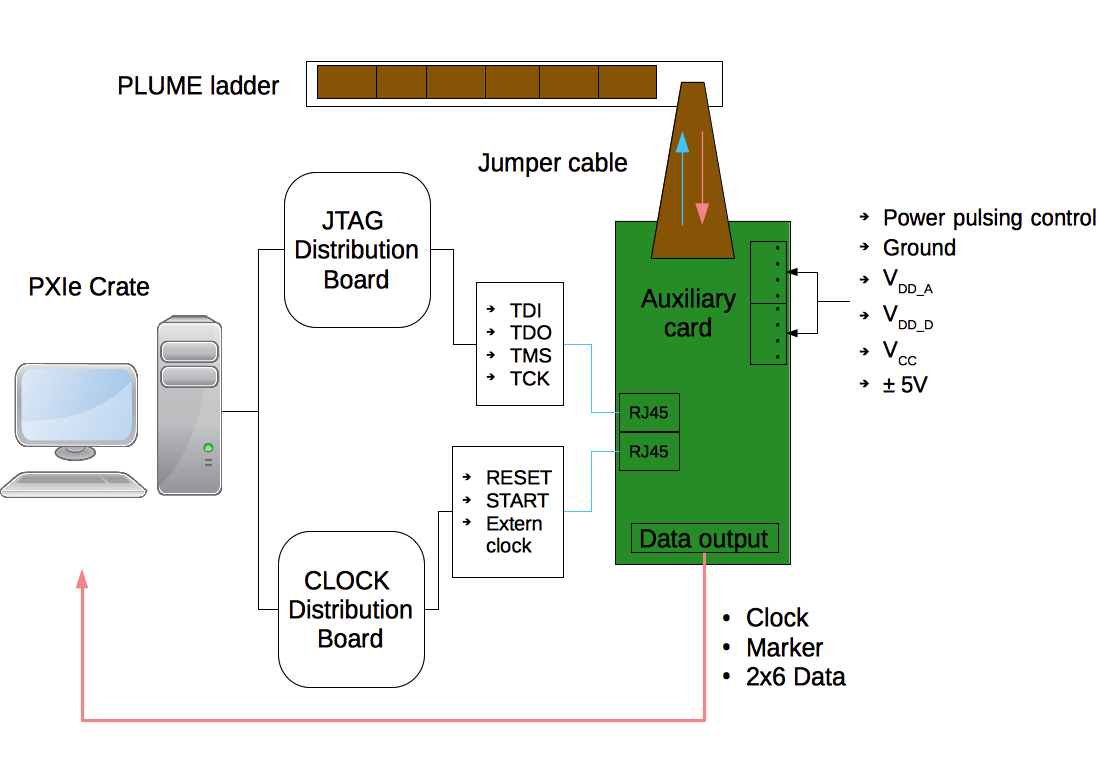
\includegraphics[width=\textwidth]{Pictures/labTests/plumeAux.png}
    \caption{Sketch of the PLUME connection scheme.}
    \label{fig:plumeAux}
  \end{figure}

  Before connecting a PLUME module to the auxiliary board, the voltages have to be set and the \gls{JTAG} communication has to be checked on the auxiliary card.
  Two external power supplies deliver $8~\rm{V}$ D.C. to the power supply board and give information on the power consumption of the whole system.
  The empty auxiliary board has a current consumption of about $350~\rm{mA}$.
  Then, $\rm{V}_{\rm{CC}}$, $\rm{V}_{\rm{DD_D}}$ and $\rm{V}_{\rm{DD_A}}$ should be at $3.3~\rm{V}$, but only the two last voltages can be adjusted by using two potentiometers on the power supply board.
  $\rm{V}_{\rm{clp}}$ is set to $2.1~\rm{V}$ and should not be outside the range $\left[2, 2.2\right]~\rm{V}$.
  \gls{JTAG} communication is verified on an oscilloscope.
  The observed signals should be:

  \begin{description}
    %\item[\gls{TDI}:]
    %\item[\gls{TDO}:]
    \item[\gls{TMS}:] by default is fixed to 1 and changes to 0 at every register selection;
    \item[\gls{TCK}:] this clock is slower (30 kHz) than the 80 MHz needed by the sensors and is dedicated to the slow control;
    \item[Reset:] by default is fixed to 1 and should change to 0 every time the reset is called by the \gls{JTAG} software;
    \item[Start:] during the test, the start signal is provided by the \gls{DAQ} software;
    \item[Clock:] independently of the method used, the 80 MHz clock has to be correctly distributed along the auxiliary card.
  \end{description}


  \subsection{Smoke test}

  After validating the auxiliary board (and with the power supplies switched off), a module can be connected to it via a jumper cable.
  Voltages applied to this module have to be adjusted again due to some dissipation inside the flex-cable and jumper cable.
  $\rm{V}_{\rm{DD_D}}$, $\rm{V}_{\rm{DD_A}}$ and $\rm{V}_{\rm{clp}}$ can be measured on different pads of the ladder: three pads are close to the connector, while the three others are at the edge of the flex-cable, as seen in figure~\ref{fig:voltagePads}.

  \begin{figure}[!tbh]
    \centering
    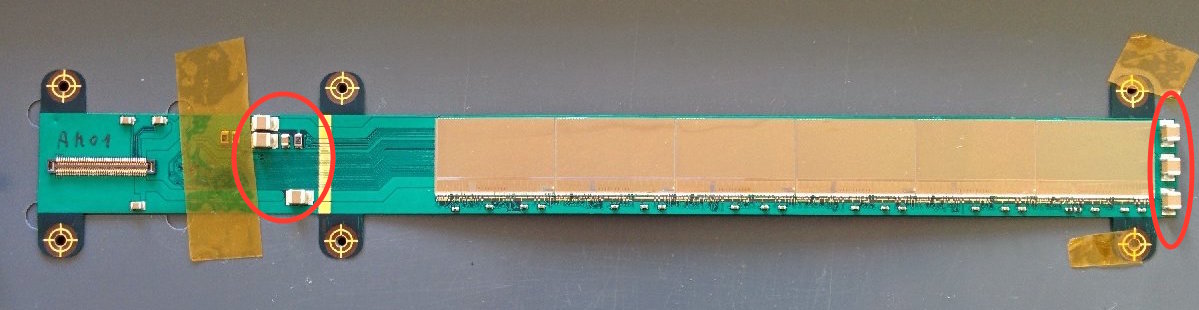
\includegraphics[width=\textwidth]{Pictures/labTests/AM01_voltagePads.jpg}
    \caption{Picture of a aluminum mirrored module with the points of measurement for $\rm{V}_{\rm{DD_D}}$, $\rm{V}_{\rm{DD_A}}$ and $\rm{V}_{\rm{clp}}$.}
    \label{fig:voltagePads}
  \end{figure}

  Two versions of jumper cable were produced, one very flexible with a high resistivity and the second one was stiff with a low resistivity.
 % The first one was not used during the test because of a problem during the fabrication.
  The most flexible cable was not used because of an important voltage drop between the auxiliary board and the module, but also because of a wrong fabrication.
  After setting the voltages to nominal values and plugging in a module, a short-circuit happened.
  The auxiliary board tests were correct and were demonstrated one more time without the module.
  Then, a thermal camera was used to find if a sensor was responsible for the short-circuit.
  One sensor was hotter than the others, although, the wire-bonds were correctly assigned.
  The problem was shown to come from a short-circuit between the $\rm{V}_{\rm{DD_D}}$ and $\rm{V}_{\rm{clp}}$ lines.
  By bypassing these two lines on the jumper cable and by connecting them directly to the module, this short-circuit has disappeared.
  The problem was solved by using a stiffer jumper cable.
  Nonetheless, any movement of the auxiliary board causes too much stress on the connector and on the flex-cable.
  Therefore, to avoid any damage, a support was built to hold the auxiliary board and the module on the same frame, thus reducing the risk of breaking anything.

  The module consumption is checked at every \gls{JTAG} step to make sure that no short-circuit occurs.
  Right after powering the system, the six sensors start in a random state and the consumption at this stage can not indicate any electrical problem.
  After the reset of the registers, the total consumption should be around $33~\rm{mA}$.
  Then, the registers are loaded and the consumption should be around $750~\rm{mA}$.
  These registers are read-back by the \gls{JTAG} software, indicating if any errors happened.
  If, during the reading step no error was discovered, the sensors can be operated and their consumption should be around $1300~\rm{mA}$.

  %Before to present the next step to control the JTAG communication of every sensor, let's introduce the MIMOSA-26 output.

  %\subsection{Mimosa-26 output}

  An inspection of the output with an oscilloscope is performed to check the slow control and to estimate the response of the sensor.
  For the normal mode data format with \gls{SUZE} enabled, the output data of the last frame are sparsified and transmitted during the acquisition of the current one.
  The information provided by the \gls{MIMOSA}-26 is contained in four output lines.
  The first output line corresponds to the \textit{clock} which is always running even if the data transmission is finished. 
  Its rate depends on the clock rate register. 
  For the normal output mode, it is $80~\rm{MHz}$.
  The second output line is the \textit{marker}, which is available in all modes.
  It is set during four clock's rising edge cycle and might be used to detect the beginning of the data transmission.
  Then, the two last output lines are dedicated to the data.
  They contain multiple information.
  First of all, the beginning and the ending of the data transmission is determined by the \textit{header} and \textit{trailer}.
  The \textit{header} and/or \textit{trailer} can be used to detect a loss of synchronisation.
  They correspond to $2 \times 16$ bits (\textit{header0-header1} and \textit{trailer0-trailer1}) and are fully configurable through the \gls{JTAG} software.
  The \textit{header} is followed by the \textit{frame counter} which corresponds to the number of frames since the chip was reset. 
  The information is separated into two words (\textit{FrameCounter0} corresponding to the least significant bit and \textit{FrameCounter1} corresponding to the most significant bit).
  Then, the \textit{data length} gives the number of 16 bits words of the useful data. 
  The useful data is split into \textit{states/line}, which contains the address of the line which has a hit and an overflow flag if the number of states is bigger than the memory limitation.
  It is followed by the \textit{state} giving the number of consecutive hits and the address of the first column.
  Finally, the \textit{trailer} is ending the data transmission followed by 32 bits of zero.
  Figure~\ref{fig:mi26Output} is a picture of an oscilloscope recording of a \gls{MIMOSA}-26 data output. From the top to the bottom, it shows the $80~\rm{MHz}$ \textit{clock}, the four clock's cycle \textit{marker}, the \textit{data0} and \textit{data1} with the \textit{header} and the \textit{frame counter}.
  More information about the \gls{MIMOSA}-26 can be found in the \gls{MIMOSA}-26 user manual~\cite{manualMi26}.

  \begin{figure}[!tbh]
    \centering
    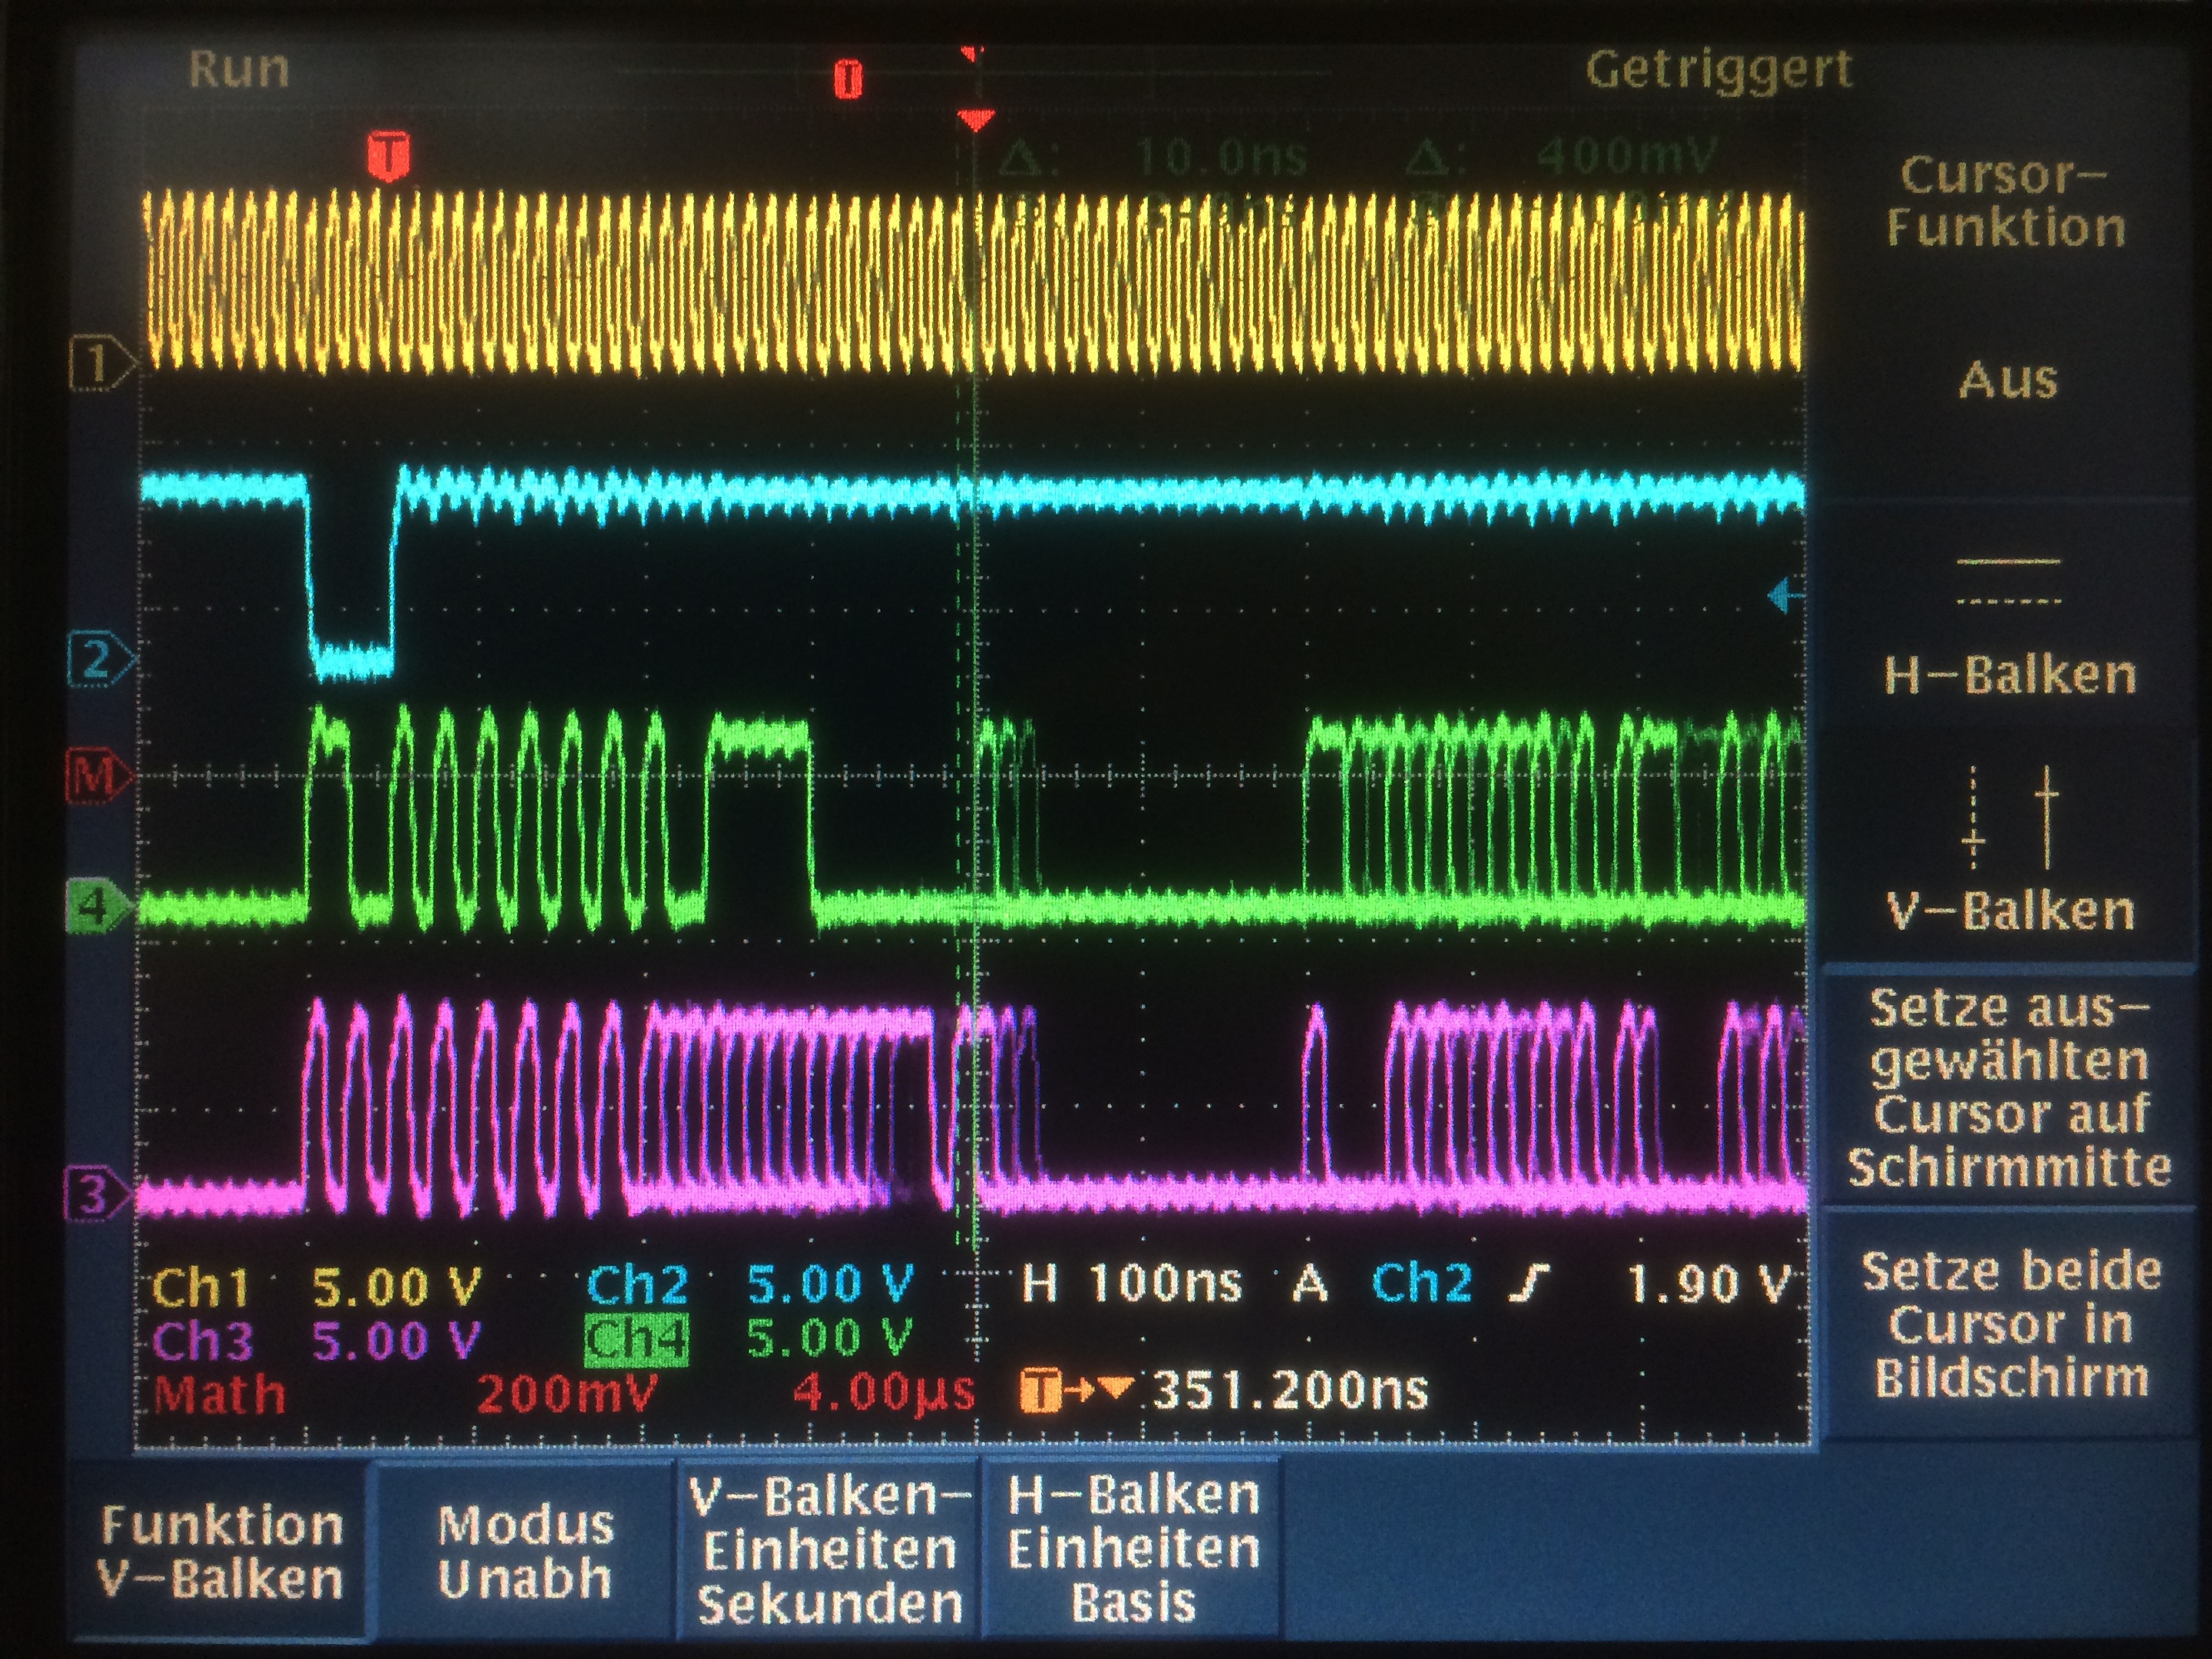
\includegraphics[width=0.8\textwidth]{Pictures/labTests/mi26_output}
    \caption{MIMOSA-26 output from oscilloscope. The top yellow line corresponds to the clock, the blue line below to the marker (which lasts 4 clock cycles), and the green and purple lines are the data output containing the hit information}
    \label{fig:mi26Output}
  \end{figure}

  \subsection{JTAG communication}

  After adjusting the voltages and looking for any short-circuits, the next step is to control the \gls{JTAG} communication for every sensor.
  Since in the \gls{PLUME} modules, all the sensors are synchronised, only \textit{clock} and \textit{marker} signals from one sensor are read back.
  On the oscilloscope, the trigger is set on the \textit{marker}.  
  The sensors are configured in the normal-mode data format (80 MHz with zero suppressed output) and the output is checked in three steps.
  First of all, the sensor is reset, the registers are loaded and read back and then the start signal is sent. 
  Through the \gls{JTAG} software, \textit{header} and \textit{trailer} are modified several times and are checked on the oscilloscope.
  Then, the discriminators' response is visualised, specifically to find pixels that always send data even if the discriminators are closed.
  The number of defective pixels and their position is then estimated.
  After that, an estimation of the threshold discriminator values to get few hits are determined and the response is checked.
  Nevertheless, using light to estimate the response of the sensor can impact the pixels' baseline and modify the normal behavior of the matrix.
  For example, instead of sending more information, the pixels are less responsive.
  Thus, using a radiation source is a better solution.

\section{Noise measurements}
\label{sec:noiseMeasurements}

  In chapter~\ref{chap:vxd}, the principle of \gls{CMOS} sensors was described and the noise of this technology was discussed.
  As a reminder, the two noise contributions are \acrfull{TN} and \acrfull{FPN}.
  \gls{FPN} is determined as an offset to be subtracted from the pixel response to reduce its non-uniformity, while \gls{TN} is coming from the contribution of different noises during the reset, the integration and the readout of the pixel.
  These noises have to be measured in the laboratory in order to find the optimum configuration to detect physics signals and reduce the noise impact on the measurement.

  \subsection{Characterisation bench}

  The noise estimation is done with a bench of characterisation composed of a National Instruments PXIe crate equipped with a 6562 digital card, two power supplies, a power distribution board, an auxiliary and a \gls{JTAG} card, as well as the module to test.
  The procedure described here is applied to a single \gls{MIMOSA}-26, or a \gls{PLUME} module, as well as a \gls{MIMOSA}-28 sensor.
  Nevertheless, the data acquisition software used during the characterisation is slightly different to match the clock speed, depending on the sensor technology.
  The four data outputs are connected from the pins on the auxiliary board to the digital card via a National Instruments spider cable.
  Firstly, a test pattern, which automatically loads a \gls{JTAG} file for this test, is used to read the \textit{header} and \textit{trailer} during several frames with a determined data length.
  It has been observed that the \textit{clock} output cable has to be $80~\rm{cm}$ longer than the three other cables to ensure the synchronisation on the rising edge.
  If this is not done or if one of the cables has the wrong polarity, the software is not able to read the \textit{header} and \textit{trailer} and the characterisation can't be done.

  Then, sensors are configured in the discriminator output mode.
  The zero suppression mode is bypassed, pixels and discriminators are in normal mode (the whole matrix is read in $115~\mu\rm{s}$), but the readout frequency is lower ($10~\rm{MHz}$).% via two \gls{LVDS} output pads.
  The control of the discriminators is divided into four sub-matrices, each containing 288 columns.
  Thus, for one sub-matrix a threshold value in /gls{DAC} units in the \gls{JTAG} software is driving all the discriminators, depending on a baseline value.
  For one line, usually one located in the middle of the matrix, its baseline response is studied to find the "middle-points" by looking for the threshold of each sub-matrix, in which the discriminators are reaching a half activation.
  When these "middle-points" are determined, the homogeneity of the matrix is checked, as shown in figure~\ref{fig:homogeneityMi26}.
  Due to the structure of the sensor, the homogeneity is not perfect and some dispersions in the discriminator response are observed between the beginning and the end of a sub-matrix.
  Moreover, to reduce this dispersion, the reference baseline, and the clamping voltage have to be adjusted.
  
  \begin{figure}[!tbh]
    \centering
    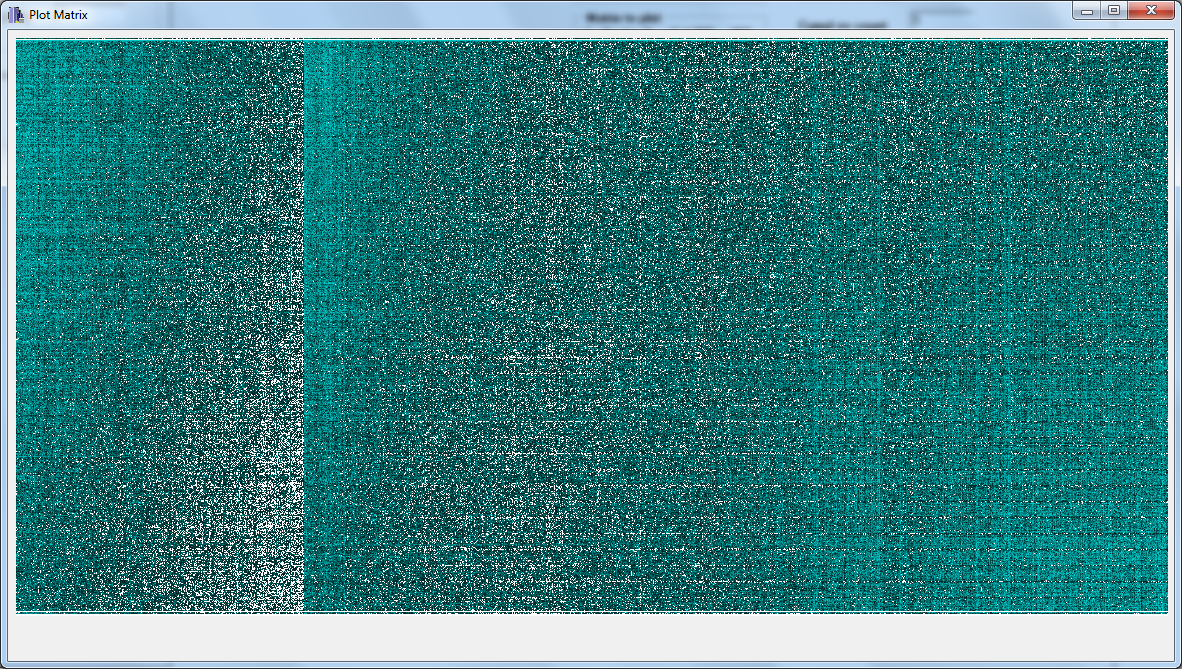
\includegraphics[width = \textwidth]{Pictures/labTests/discri_middle.png}
    \caption{Matrix response for the discriminators half activated.}
    \label{fig:homogeneityMi26}
  \end{figure}
  
  Afterward, the thresholds are set to the lowest and highest value to look for defective pixels in the matrix.
  On the one hand, few pixels can be always activated even if the discriminators were closed.
  Figure~\ref{fig:openPixel} depicts the matrix output for when all the discriminators are closed.
  Therefore, a line is always activated, as well as a few pixels in a column and they are increasing the fake hit rate of the matrix.
  A solution exists to disconnect some discriminators in order to reduce the noise of defective columns on the \gls{JTAG} program, nevertheless, no solution during the sensor programming exists to remove the defective lines.
  On the other hand, a few pixels can be always deactivated even if the discriminators are completely opened, i.e these pixels are not able to detect any physics signal.
  This behavior is represented in figure~\ref{fig:closePixel}. 
  To date, no solution exists to make these pixels working properly.
   
  \begin{figure}[!tbh]
    \centering
    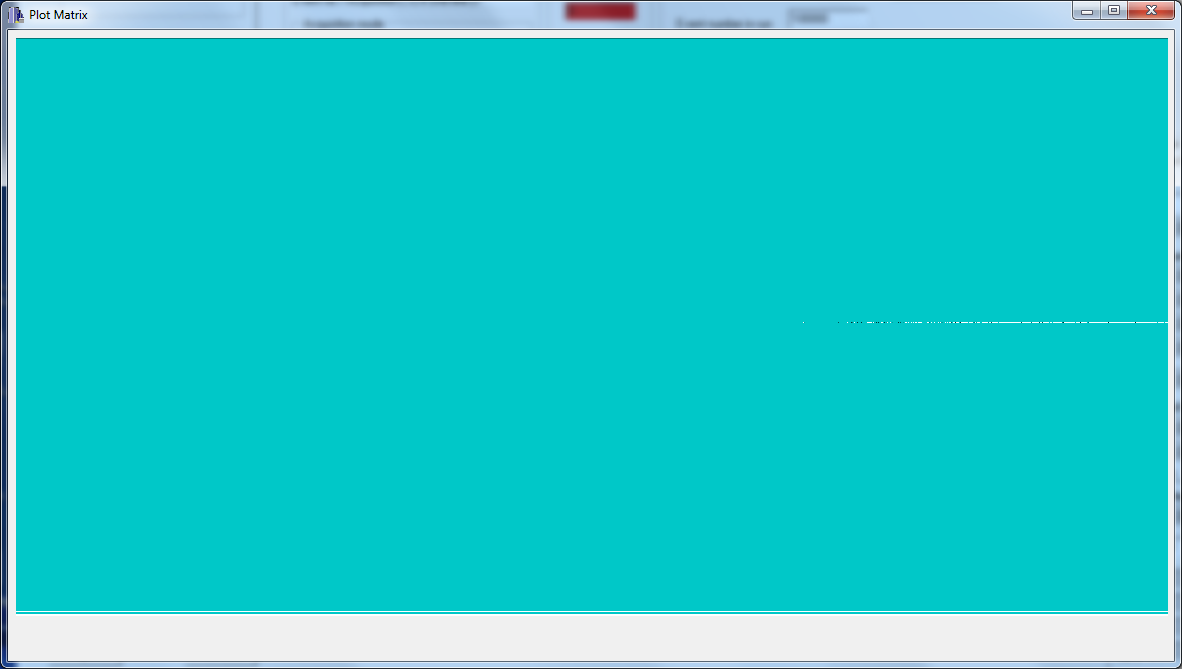
\includegraphics[width=\textwidth]{Pictures/labTests/th0.png}
    \caption{Matrix response in discriminator mode, where all the discriminators are opened. On the right of the matrix, one row is not working correctly and some pixels are never activated}
    \label{fig:openPixel}
  \end{figure}
   
  \begin{figure}[!tbh]
    \centering
    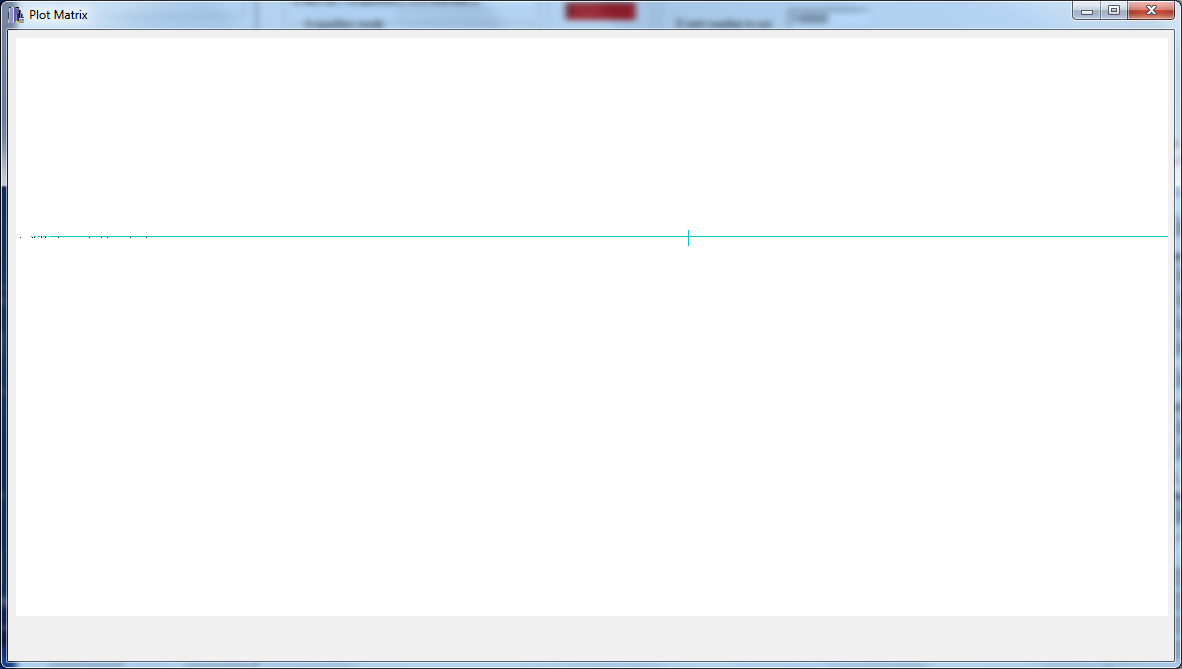
\includegraphics[width=\textwidth]{Pictures/labTests/th255.png}
    \caption{Matrix response in discriminator mode, where all the discriminators are closed. One line of pixels is always activated, as well as few pixels in one column. This will increase the fake hit rate of the sensor.}
    \label{fig:closePixel}
  \end{figure}

  \subsection{Threshold scan}

  The noise performance of the sensor is determined through a threshold scan around the "middle-point" found before.
  This threshold scan consists of recording the normalised response of the discriminators or the discriminators and the pixels for different threshold values.
  For the first possibility, an external voltage is injected into the discriminators while the pixels are disconnected.
  Only the noise contribution coming from the discriminator is thus determined.
  In this work, the noise performance results presented were done without injecting an external voltage, but rather with the sensitive system connected to the discriminators.
  Usually, 29 runs containing between 500 to 1000 events are stored.
  The files created are used to firstly build a configuration file containing the \gls{DAC} values of each sub-matrix for the different thresholds applied.
  The threshold is here defined as the voltage applied to the discriminators.
  Afterward, this file is analysed and converted to create an output file containing a hit average picture of each sub-matrix for each step.
  Then, a macro based on C++ and the ROOT framework is reading the hit average picture to plot the transfer function, also called "S" curve, as represented in figure~\ref{fig:transfer}.
  It shows the normalised response of the 288 discriminators and the pixels contained in this sub-matrix as a function of the threshold applied in millivolts.
  The temporal noise of each pixel is calculated from the derivative of the "S" curve and is represented here in the left plot of figure~\ref{fig:TN&FPN}.
  The mean value of the distribution obtained the mid-point threshold of a pixel.
  The dispersion of the mid-point threshold corresponds to the fixed pattern noise, represented on the right plot of figure~\ref{fig:TN&FPN}.
  
  \begin{figure}[!tbh]
    \centering
    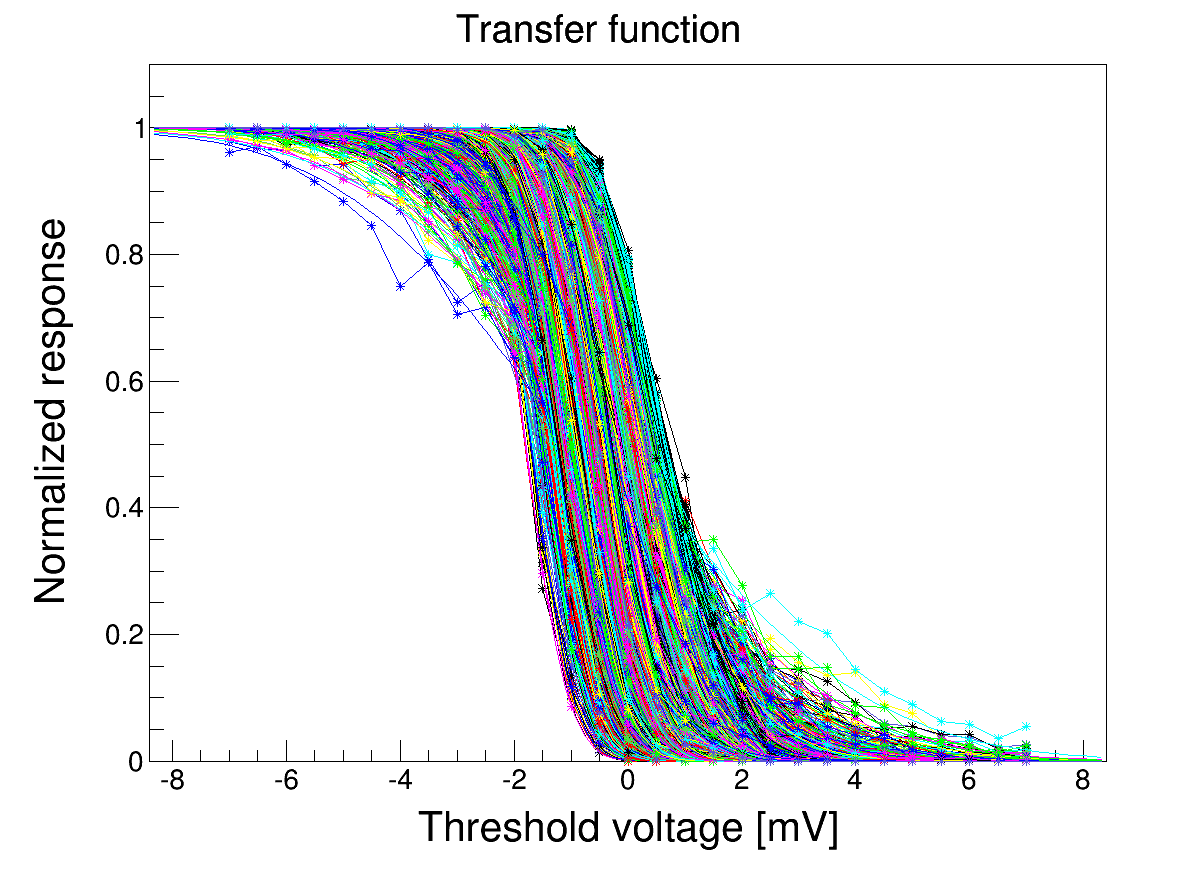
\includegraphics[width=0.7\textwidth]{Pictures/labTests/transfer_B.png}
    \caption{Pixels response of a threshold scan around the middle-point of discriminators for a sub-matrix.}
    \label{fig:transfer}
  \end{figure}

  \begin{figure}[!tbh]
    \centering
    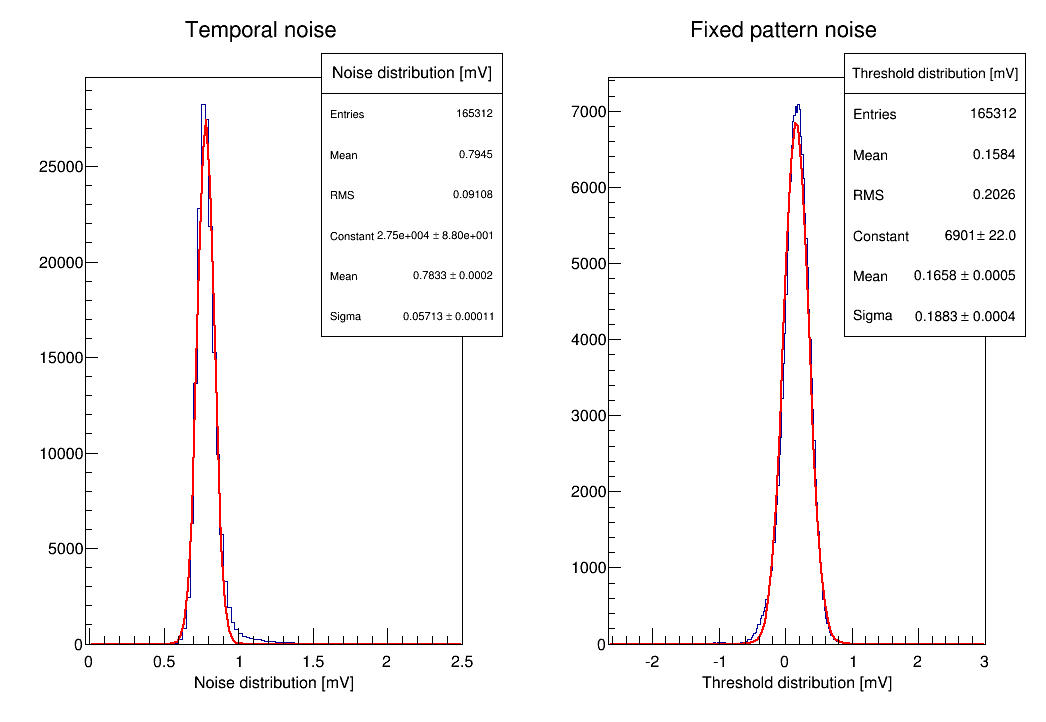
\includegraphics[width=0.8\textwidth]{Pictures/labTests/noise_A.png}
    \caption{Noise performances of a sub-matrix for the discriminators and the pixel array output. The temporal noise is plotted on the left plot, whereas the fixed pattern noise is represented on the right plot.} 
    \label{fig:TN&FPN}
  \end{figure}

  The plot on the left in figure~\ref{fig:TN&FPN} represents the temporal noise, while the right one represents the fixed pattern noise.
  The systematic offset of the discriminator is extracted from these measurements (the mean value of the temporal noise, the mean value and the sigma value of the fixed pattern noise).
  To calculate the discriminator thresholds of each sub-matrix for a given \acrfull{SNR}, the total noise is determined as:
  
  \begin{equation}
    \rm{Total~noise} = \sqrt{\langle\rm{TN}\rangle^2 + \langle\rm{FPN}\rangle^2},
  \end{equation}

  with $\langle\rm{TN}\rangle$ the mean value of the temporal noise, and $\langle\rm{FPN}\rangle$ the mean value of the fixed pattern noise.

  For a given S/N cut $\sigma$, the thresholds are determined by:

  \begin{equation}
    \rm{Threshold~(mV)} = \rm{Total~Noise} \times \sigma + \rm{offset}.
  \end{equation}

  This is converted into the \gls{DAC} values by taking into account the \gls{DAC} offset and the \gls{DAC} slope, which is assumed to be $0.25~\rm{mV}$:
  
  \begin{equation}
    \rm{Threshold~(DAC)} = \frac{\rm{Threshold~(mV)} - \rm{DAC}_{\rm{offset}}}{\rm{DAC}_{\rm{slope}}}.
  \end{equation}

  \subsection{Noise measurements}

  Once the thresholds are defined for the different cuts, the fake hit rate of the matrix, as well as the detection homogeneity is determined.
  A quick step consists of using the \gls{DAQ} software and acquiring $10^4$~events in the dark to determine the noise qualitatively. 
  The fake hit rate per event per pixel is then defined as:

  \begin{equation}
    \rm{F.H.R} = \frac{\rm{Number~of~hits}}{\rm{Number~of~events} \times \rm{Number~of~pixels}}. 
  \end{equation}
  
  Figure~\ref{fig:darkEvents} represents the accumulation in the dark of $10^4$~events for a threshold five times bigger than the noise.
  The measured fake hit rate was below $10^{-4}~\rm{hits/pixel/event}$.

   \begin{figure}[!tbh]
    \centering
    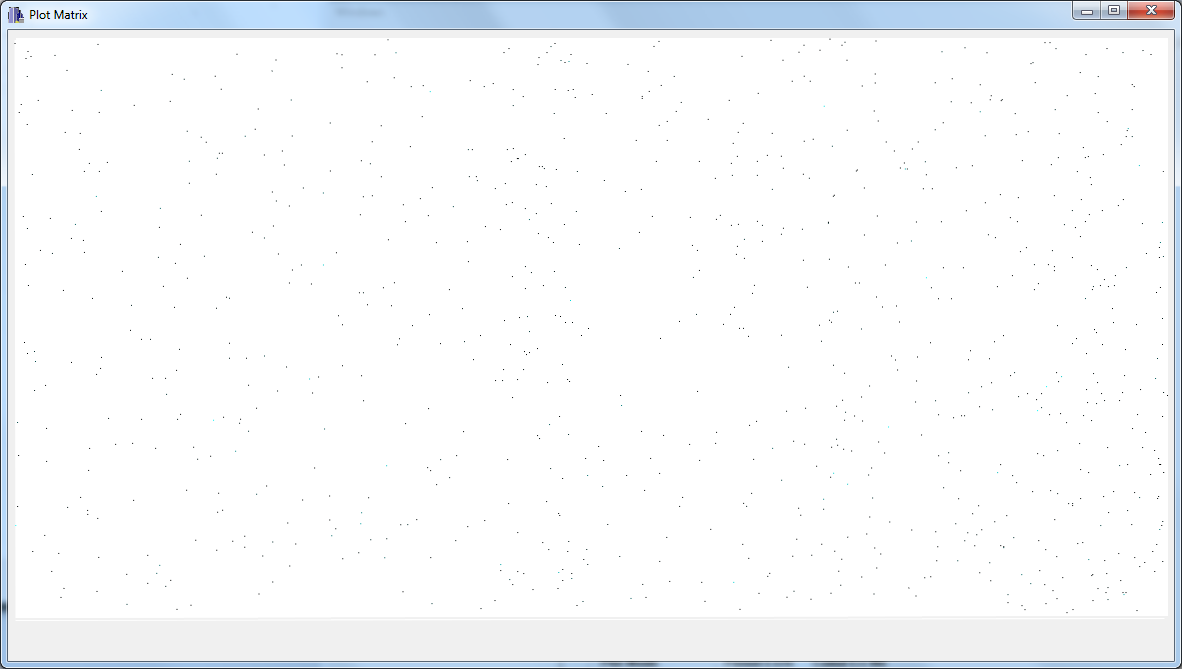
\includegraphics[width=0.6\textwidth]{Pictures/labTests/dark_10kEvents_not_noisy.png}
    \caption{Accumulation of $10^4$ events at a thresholds of 5 times the noise acquired in the dark for one sensor.}
    \label{fig:darkEvents}
  \end{figure}

  Then, an iron $^{55}\rm{Fe}$ source is used to control the homogeneity of the thresholds determined before.
  Figure~\ref{fig:fe55} represents the accumulation of ten thousand events for a threshold five times larger than the noise with an iron source on top of the sensor.
  
  \begin{figure}[!tbh]
    \centering
    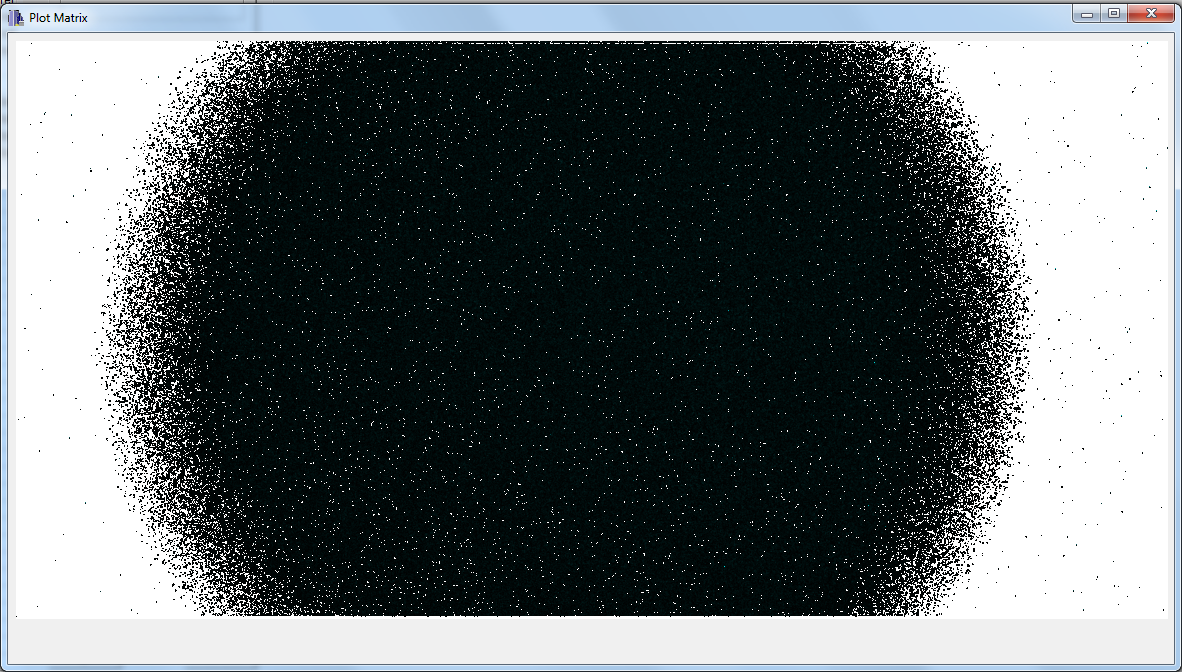
\includegraphics[width=0.6\textwidth]{Pictures/labTests/10kEvents_Fe55_cut5sigma.png}
    \caption{Accumulation of $10^{4}$ events at a threshold of 5 times the noise with a $^{55}\rm{Fe}$ radiation source for one sensor.}
    \label{fig:fe55}
  \end{figure}

  Finally, in order to validate the sensor, the acquisition system used during the test beam is used to calculate quantitatively the fake hit rate.
  The auxiliary board is connected to a Flex RIO board instead of the digital card.
  The test beam \gls{DAQ} software developed by the \gls{IPHC} is using a LabVIEW interface for the run control.
  It provides a lot of useful pieces of information, such as the number of events acquired, the \textit{header}, the \textit{trailer} and the \textit{frame counter} of the sensor.
  This helps the user to know if the acquisition is running properly.
  If the \textit{frame counter} is different for each sensor, this points at a loss of synchronisation during the acquisition.
  Also, a different \textit{header} or \textit{trailer} such as the ones set in JTAG software might point out a wrong connection.
  A second  piece of software is used to store the data into three files: a parameter file containing the run number, the event number, an index file and a binary file containing the raw data.
  Two acquisition modes are available. 
  The first one, used in the test beam, acquires data only when a trigger is sent.
  The second one stores all frames regardless of the trigger status. 
  This acquisition is the one used in the lab, when only the noise of the sensor is measured.
   
  Several runs each containing one million events are acquired for different thresholds. 
  The data stored are analysed with software developed by the \gls{IPHC} called \gls{TAF}~\cite{TAF2015}.
  It is based on C++ and the ROOT framework.
  The software reads the information of the hit pixels, reconstructs the clusters of hit pixels and in the case of a test beam is able to reconstruct tracks from the hit information.

  The fake hit rate is determined with respect to the number of pixels hit per event.
  From the fake rate distribution per pixel shown in figure~\ref{fig:pixel/event} (bottom-left plot), which represents the number of pixels fired per event, the average fake hit rate is calculated as the mean of this distribution divided by the total number of pixels contained in the matrix.
  \begin{figure}[!tbh]
    \centering
    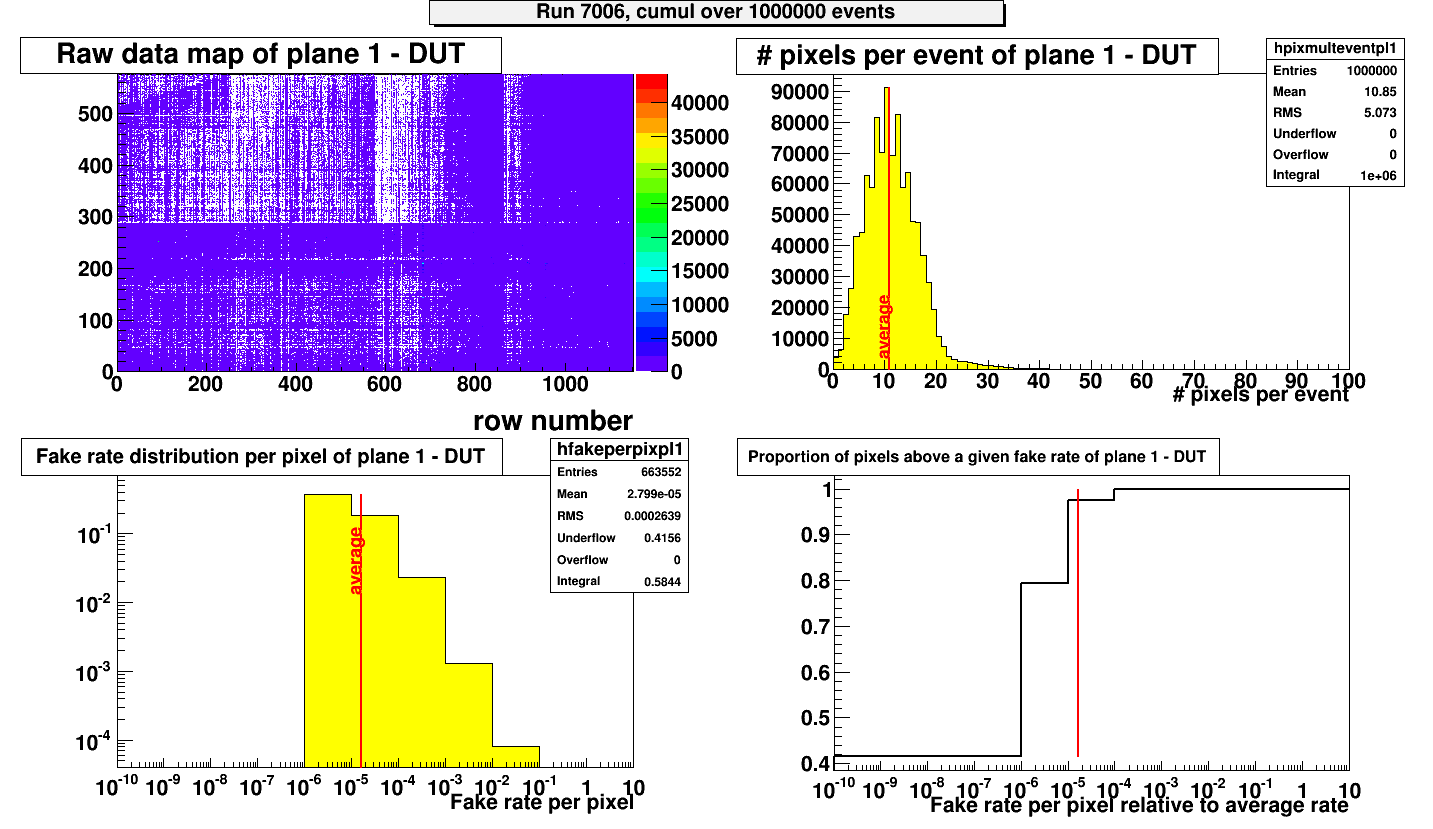
\includegraphics[width = \textwidth]{Pictures/labTests/FHR_AS01_chip3.png}
    \caption{Results of the fake hit rate measurement for a threshold three times bigger than the noise. The top left plot represents a raw picture of the million events accumulated over the whole matrix. The top right one is the distribution of the number of pixels hit per event. The bottom left plot is the fake hit rate per pixel distribution, while the bottom right one is the fake hit rate relative to the average rate distribution.}
    \label{fig:pixel/event}
  \end{figure}
  The error on the measurement is then the root mean squared of the distribution divided by the number of entries and the number of pixels inside the matrix.
  This calculation is done for different thresholds and figure~\ref{fig:FHR} represents the average fake hit rate per pixel per event as a function of the threshold for one sensor of an aluminum module.
  These results match the expected behavior for a standalone \gls{MIMOSA}-26 sensor as shown in figure~\ref{fig:mi26Perf}.

  \begin{figure}[!tbh]
    \centering
    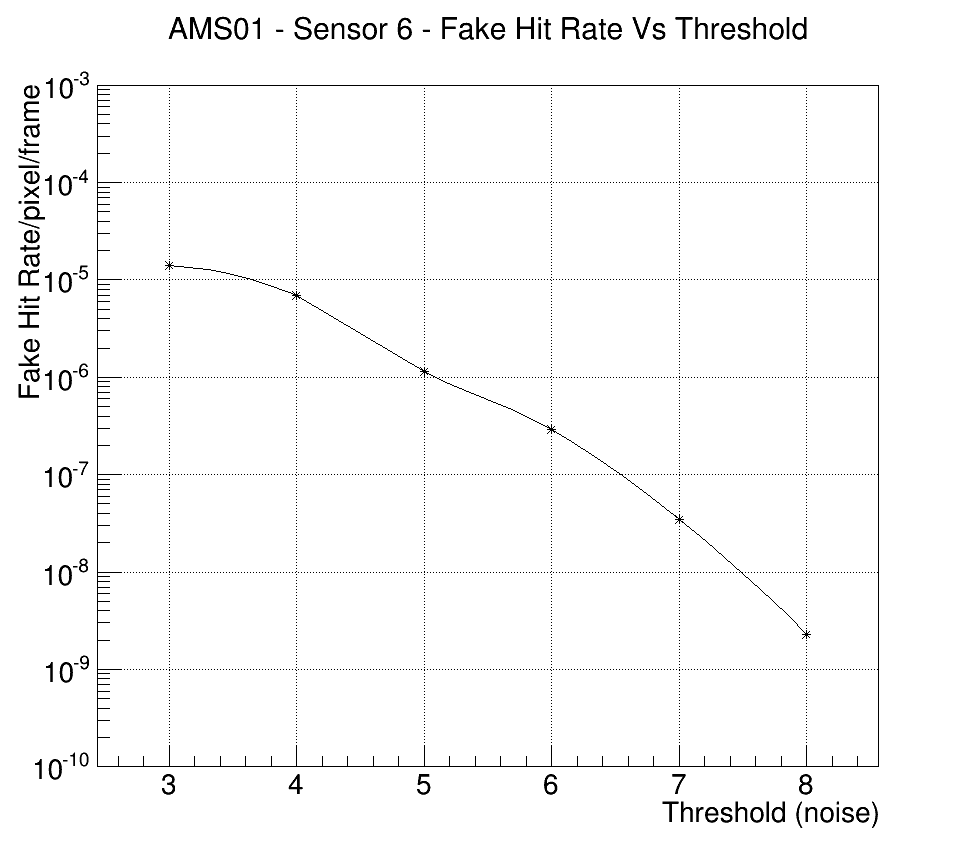
\includegraphics[width=0.7\textwidth]{Pictures/labTests/fake_sensor6.png}
    \caption{Distribution of the fake hit rate per pixel.}
    \label{fig:FHR}
  \end{figure}

\section{Conclusions}

  The assembly procedures and tests performed in the laboratory were introduced through this chapter.
  Only results for one sensor were presented, but several modules were tested. 
  All of them behave the same as the one expected for one single \gls{MIMOSA}-26.
  So far, for new \gls{PLUME} versions which have a narrower flex-cable and which should embed only $0.35~\%$ of the radiation length, different prototypes were built. 
  The first ladder using copper module was assembled in January 2016.
  New ladders are currently being built and the collaboration is expecting to test them at the \gls{DESY} test beam facility in 2017.
  Nevertheless, aluminum ladders seem to be more challenging to build.
  The three first mirrored versions produced have a problem with the \gls{ZIF} connector.
  It could have been damaged by plugging and unplugging the jumper cable.
  This problem did not occur with copper mirrored versions and this might come from a more fragile flex-cable.
  Ideally, each module should have is own jumper cable, which then should not be disconnected.
  Nevertheless, for shipping them, there is no other solution.
  The collaboration is thinking of a tool which will reduce the stress applied to the connector.

  The next chapter deals with the tests performed under realistic conditions at the CERN-SPS facility with the PLUME-V1 prototype in 2011.

    \chapter{Determination of the material budget}
\label{chap:X0}

  The discovery of new physics and the characterisation of the already known particles are possible only with performant detectors.
  As it was presented on chapter~\ref{chap:vxd}, the fabrication of a vertex detector is constrained by two parameters: the pointing resolution and the material budget.
  The first fully functional prototype of \gls{PLUME} was tested in November 2011 at CERN with 120 GeV pions.
  The results have shown that the pointing resolution of the ladder corresponds to the expected value for the \gls{ILD} and moreover, the use of a double-sided structure improves this pointing resolution. 
  Nevertheless, the material budget ($\rm{X}_0$) of such device is estimated only by calculation and the SPS beam is not suited to a material budget measurement.
  Therefore, a test beam campaign of the PLUME-V1 prototype was done in April 2016 at DESY test beam 21 with positrons up to 5 GeV.
  Firstly, the test beam preparation is discussed.
  Then, the motivation, the test beam facility, as well as the tools used for the analysis are presented.
  Finally, the results on the radiation length measurements are discussed.
  %The reason to test an already known prototype is that the performances have to be the same at low and high-momentum particles.
  %The preparation of the test beam is firstly discussed.
  %Then, the test beam facility, as well as the tools used for the analysis are presented.
  %Finally, the radiation length measurements are discussed..

  %The first fully functional prototype of \gls{PLUME} was tested in November 2011 at CERN with 120 GeV pions. 
  %Due to the environment, the ladder has to be able to track high momentum particles, as well as ones with low momentum.
  %The material budget on the sensitive area for incoming particles is estimated to be about 0.65 \% $X_0$.

\minitoc

  \section{Preparation of the test beam}

  In April 2016, a test beam campaign with electrons and positrons up to 5 GeV was performed at the DESY-II test beam facility.
  The preparation of a test beam campaign is a long, intense and stressing period.
  The different aspects of the test beam have to be carefully though to minimise the problems and the time spent for debugging during the test period.
  This consists to schedule precisely the different measurements that have to be performed during the restricted time, as well as the set-up to use, the integration of the \gls{DUT} and the acquisition system to use.
  
  %The first fully functional PLUME ladder (PLUME-V1) was tested again to study the performances of this device with low-momentum particles.
  %The different measurements scheduled are presented here, as well as the preparation of the test beam, from the PLUME integration to the data acquisition.

  % A second test beam was performed in April 2016 at DESY with positrons up to 5 GeV. 
  % The goal of this test beam was to study the performances of this device with low-momentum particles.
  % The ladder tested is a second PLUME-V1 prototype.
  % The steps, from the preparation to the analysis are explained here.
  % Different measurements were planned to fully test the ladder.
  % Nevertheless, as this test beam was at the end of my Ph. D., I could not perform all the measurements.
  % The preparation are presented for all the measurements, but the analysis itself is focused only on the radiation length measurement.

    \subsection{Measurements and telescope configuration}

    During the two weeks of test beam available, the measurements planed consist, firstly, to validate the characteristics of the ladder for low momentum particles, such as the spatial resolution, the efficiency or the benefits of the mini-vectors.
    Runs with different tilts (from $0^{\degree}$ to $60^{\degree}$ with a step of $10^{\degree}$) and different air flow speeds for the cooling system ($3~\rm{and}~6~\rm{m.s}^{-1}$) are performed to study again the deformations of the ladder.
    Finally, for the first time, the radiation length of \gls{PLUME} is measured to compare it to the theoretical estimations, which gives $\rm{X_{0}} \simeq 0.65~\%$ for the version tested.
    Although many runs were acquired to performed the different measurements, the test beam was scheduled at the end of my Ph. D.
    Therefore, I am not able to perform a complete analysis of the first prototype for low momentum electrons.
    The section~\ref{sec:X0} presents the study I have performed on the radiation length measurement.

    A second aspect of the test beam is to determine the geometry of the reference planes to optimise the pointing resolution of the telescope.
    This depends on the spacing between the different planes and the position of the \gls{DUT} respectively to the telescope.
    The best resolution is achieved by placing the inner planes of the telescope as close as possible to the \gls{DUT} and the outer planes as far as possible from the \gls{DUT}.
    Because of the deformation study, which needs to rotate the ladder, the inner planes can not be pressed to the \gls{DUT} without modifying the geometry at each steps.
    Hence, to keep a consistent alignment and to reduce the time spending on the off-line alignment, it was decided to fixed the inner planes as close as possible to be able to rotate the ladder without modifying the geometry.
    Moreover the ladder is not centered in its box, so to keep an equal distance between the two sides of the ladder and the two inner planes, the minimal distance between the telescope planes are calculated by taking into account an offset.

    %The telescope has a better pointing resolution when the inner planes are very close to the \gls{DUT} and the outer planes are far away from it.
    %Nevertheless, to perform the deformation measurements and to tilt the \gls{DUT} without moving the telescope planes at every angle and performing the alignment steps one more time, the two inner planes have a distance of ....
    %Moreover, the ladder is not placed in the middle of the box, thus, the distance between one inner telescope plane to the box is different from the distance between the other side and other telescope plane.

    For the first time, the collaboration has decided to use the EUDET telescope and EUDAQ for the acquisition, instead of the Strasbourg telescope and the IPHC acquisition.
    Several configuration are available for the set-up used.
    The first ones consist to use the six planes of the EUDET telescope and to have two separate acquisitions, one for \gls{PLUME} and the second one dedicated for the telescope and then, to merge the data together.
    As the EUDET telescope is equipped with the same sensors as \gls{PLUME}, the acquisition can be simplified by having only four telescope planes and connecting directly two sensors of the \gls{DUT}.
    A simulation toolkit developed by Simon Spannagel\cite{spannagel_2016_48795} and based on \gls{GBL} is used to compare the pointing resolution at the \gls{DUT} position for different telescope geometries.
    Here, the six and four telescope planes set-ups are compared for different energies and spacing between the sensors.
    This simulation takes into account the material budget of the telescope, the \gls{DUT} and the multiple scattering of electrons in the air.
    One telescope plane as a material budget of $0.053~\%$ of $\rm{X_{0}}$, whereas \gls{PLUME} is $0.65~\%$ plus two kapton foils used to insulate the ladder from the light ($\sim 0.71~\%~\rm{X_{0}}$).
    For both configurations, the telescope is divided into two arms, two or three planes on each side of the \gls{DUT}.
    The maximal distance between each plane of one frame is $d_{\rm{max}} = 150~\rm{mm}$ for the six sensors configuration, whereas for the second one it is $d_{\rm{max}} = 300~\rm{mm}$.
    
    \begin{table}[!h]
      \centering
      \begin{tabular}{c c c}
        \hline %----------------------------
        \multirow{2}*{Energy (GeV)} &  \multicolumn{2}{ c }{$\sigma_{\rm{res}}~\rm{(\mu m)}$} \tabularnewline
                              &  4 planes & 6 planes \tabularnewline
        \hline %----------------------------
        \hline %----------------------------
        2 & 4.85 & 4.78 \tabularnewline
        3 & 3.79 & 3.83 \tabularnewline
        4 & 3.35 & 3.40 \tabularnewline
        5 & 3.12 & 3.15 \tabularnewline
        6 & 2.98 & 2.99 \tabularnewline
        \hline %----------------------------
      \end{tabular}
      \caption{Estimation of the resolution measured $\sigma_{\rm{res}}$ at the DUT position for a telescope with four planes and six planes.}
      \label{tab:estimationRes}
    \end{table}

    The table~\ref{tab:estimationRes} summarises the measured resolution at the \gls{DUT} position for different energies and the use of four or six telescope planes does not have an impact on the telescope pointing resolution.
    The figure~\ref{fig:estimationRes4.7GeV} displays the pointing resolution as a function of the different spacing between two telescope planes of the same frame, for an energy set to $4.7~\rm{GeV}$.
    %Several solutions were available.
    %The first one consists to use the six telescope planes of EUDET and a separate acquisition for \gls{PLUME}.
    %As the acquisition is limited to six inputs and the ladder requires at least one sensor on each side to be acquired, a solution to merge the data has to be thought.
    %As the EUDET telescope and \gls{PLUME} are equipped with the same sensors, the acquisition can be simplified by having only four telescope planes and connecting directly two sensors of \gls{DUT}.
    %A simulation tool was used to define which configuration is giving the best pointing resolution at the \gls{DUT} positions.
    %This toolkit was developed by Simon Spannagel and is based on \gls{GBL}.
    %For different energy, the resolution at the PLUME position was calculated for a set-up with four telescope planes and a set-up with six.
    %The material budget of the \gls{DUT} is determined by the material budget of \gls{PLUME} plus two kapton foils used to insulate the ladder from light.
    %For both configuration, the telescope is made of two arms on each side of the \gls{DUT}.
    %With six sensors, the maximal distance between each plane of one frame is $d_{\rm{max}} = 150~\rm{mm}$, whereas for the four sensors configuration it is $d_{\rm{max} = 300~\rm{mm}}$.

   % The results shown on figure~\ref{fig:estimationRes4.7GeV} depicts the measured resolution at the position of the \gls{DUT} as a function of the distance between two telescope planes of the same arm.

    \begin{figure}[!h]
      \centering
      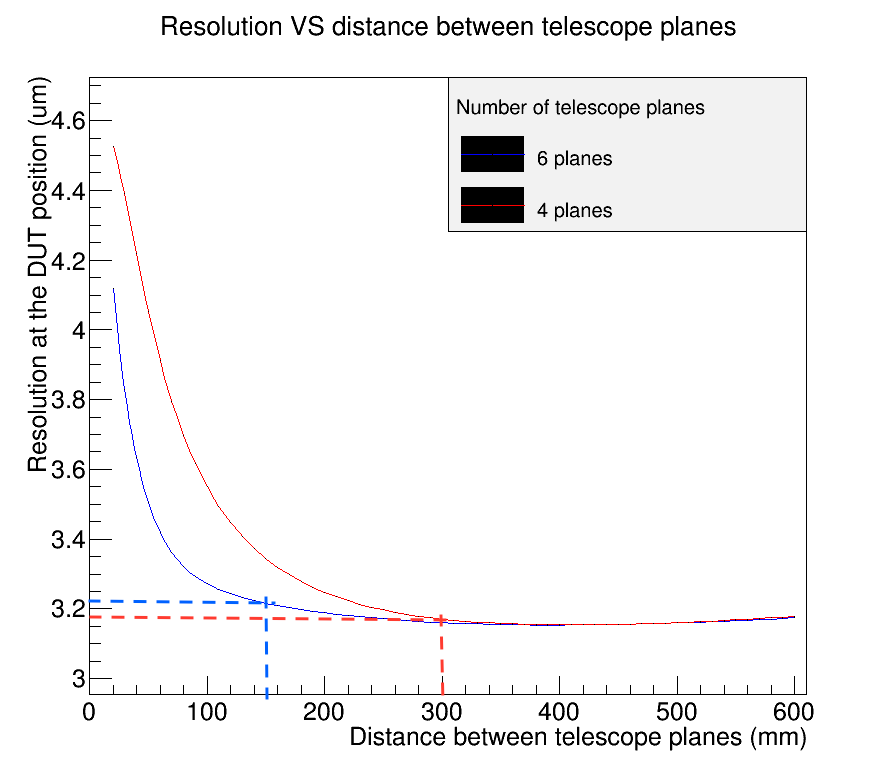
\includegraphics[width = 0.7\textwidth]{Pictures/X0/resolution_4Vs6planes_4-7GeV.png}
      \caption{Estimation of the resolution measured at the DUT position as a function of the distance between two telescope planes of the same arm.
      The blue lines is the results for six planes, whereas the red line is for four planes. 
      The dashed lines are the maximal distance between two planes due to the rail limitation of the telescope frame.}
      \label{fig:estimationRes4.7GeV}
    \end{figure}

    As the number of telescope planes does not impact the pointing resolution, it has been decided to use only four telescope planes and two \gls{PLUME} sensors (one on each side) to simplify the acquisition system.
    %The sensors of the telescope and \gls{PLUME} are both \gls{MIMOSA}-26 thinned down to $50~\rm{\mu m}$.
    %Instead of building a DAQ compatible with EUDAQ, two EUDET telescope planes are removed from the set-up and replaced by two \gls{PLUME} sensors (one on each side).
    However, the synchronisation and the stability of the acquisition have to be tested before the test beam campaign. 

    \subsection{Acquisition system and experimental set-up}
      
      \subsubsection{EUDAQ}

      EUDAQ is a modular cross-platform data taking framework developed for the EUDET-type beam telescopes\cite{Jansen}.
      It is designed to be flexible and to have an easy integration of other devices.
      The software is based on \textit{producers}, that are linked between the different subdetector systems, such as the beam telescope, the \gls{DUT} user DAQ and the \gls{TLU}\cite{Cussans2009}.
      The events of each subdetector are then correlated to form one single global event for data belonging to one trigger.
      This step is done by the \textit{Data Collector}.
      The robustness of the acquisition set-up planed is tested by performing multiple runs for multiple configuration in the laboratory.
      The data are acquired with only the \gls{PLUME} to ensure that EUDAQ can cope it, and then single \gls{MIMOSA}-26 sensors are added and runs of several hours are performed to look for a loss of synchronisation.

      \subsubsection{Experimental set-up}

      Finally, the integration of \gls{PLUME} for the different measurements to perform is investigated.
      For the deformation studies, the \gls{DUT} is mounted on a rotation stage. 
      With respect to the local coordinate system (or sensor coordinate system), the rotation is along the $u$-direction. 
      The first option considerer to performer the rotation is to orient the ladder in the same direction as the telescope's sensors. 
      Hence, the ladder is in the horizontal position and the rotation needs a complicated frame to ensure the stability of the system.
      The weight of the box and ladder is applied only on the rotation stage. 
      Due to the complexity and the time needed to build this frame, a second option has been considered.
      The ladder is placed vertically on a rotation stage. 
      There is a $90^{\circ}$ rotation between the telescope sensors and the \gls{PLUME} ones.
      The frame consists of an insulated aluminum plate on which the \gls{DUT} sits.
      To avoid to damage the \gls{DUT} during the test beam, the flex-cable is maintained on the frame by two clamps.
      In this way, less constraint are applied on the connector. 
      A plate with screws hold the ladder strongly to the frame.
      The frame is then mounted onto a rotation stage, which is mounted on a translation stage.
      The figure~\ref{fig:mechanics} shows a schematic model of the frame designed and built at DESY.
      
      \begin{figure}[!h]
        \centering
        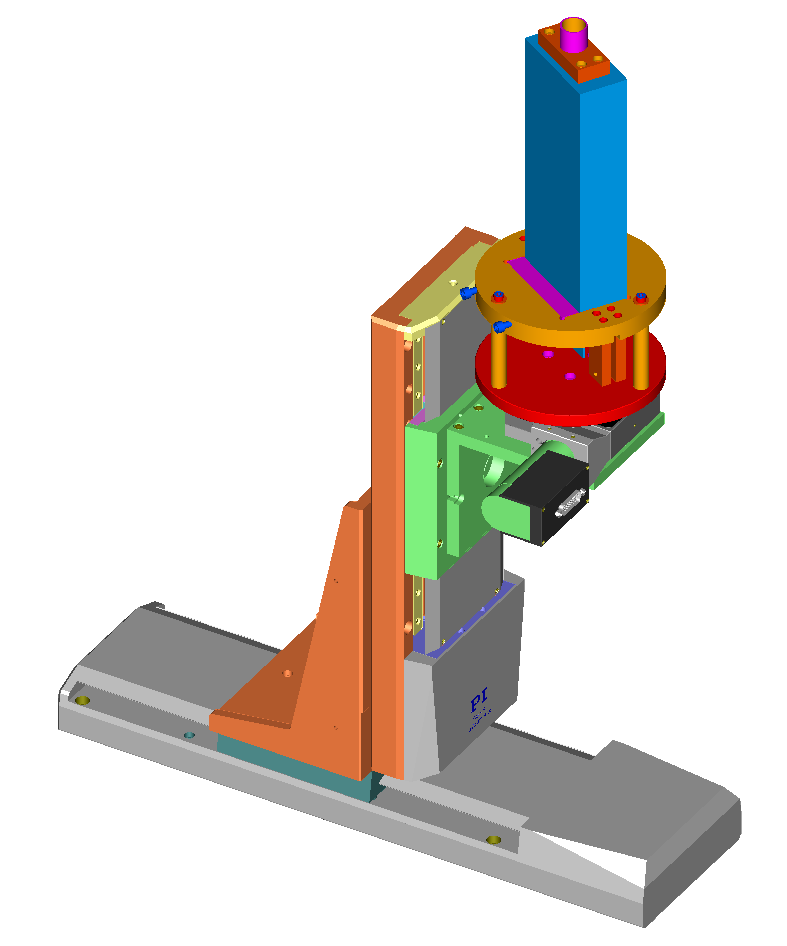
\includegraphics[width = 0.5\textwidth]{Pictures/X0/Frame/Testbeam1.PNG}
        \caption{TCAD model of the mechanical structure designed for the test beam in April. The ladder is hold on a circular frame fixed to a PI rotation stage, mounted onto a XY-table.}
        \label{fig:mechanics}
      \end{figure}

      To control the heating of the ladder during the test beam, a cooling system consisting of a simple fan is used.
      On one endcap, a pipe is fixed and connected to the fan.
      Some studies in Strasbourg were done to determine the air flow speed as a function of the voltage applied.
      Hence, an air flow speed of $3~\rm{m.s^{^1}}$ is achieved with $5~\rm{V}$ and an air flow speed of $6~\rm{m.s^{-1}}$ for $10~\rm{V}$.
      This values result in an operating temperature of all sensors between approximately $40^{\degree}\rm{C}$ and $52^{\degree}\rm{C}$.

      During the test beam campaign, the \textit{clock} and \textit{marker} are read from one sensor of \gls{PLUME}.
      The \textit{clock} is extended with a $80~\rm{cm}$ long cable to ensure that one frame starts on the rising edge.
      The second input of the acquisition is a \gls{PLUME} sensor (opposite side of the first sensor), followed by the four telescope planes. 
      Moreover, \gls{PMT}s are placed in coincidence on each side of the telescope.
      They are used to trigger the acquisition only when the beam passes through the entire set-up.
      Hence, the fake events are reduced and the data stream is smaller.

      %To ensure the synchronisation of the ladder and the telescope planes, the acquisition is synchronised on the \textit{clock} provided by one of the \gls{PLUME} sensor.
      %In the lab, two MIMOSA-26 sensors and the ladder to test are plugged together to the NI-crate. 
      %Runs of several hours are launched to verify the synchronisation.
      %As the \gls{DUT} and telescope planes are connected to the same \textit{JTAG} card and \textit{clock} distribution board, the start signal arrives at the same time on each sensor.
      %If a delay appears, there is a loss in the synchronisation and the acquisition does not work anymore.
      %The frame-counter should be the same on each sensor.

    \begin{figure}[!h]
      \centering
      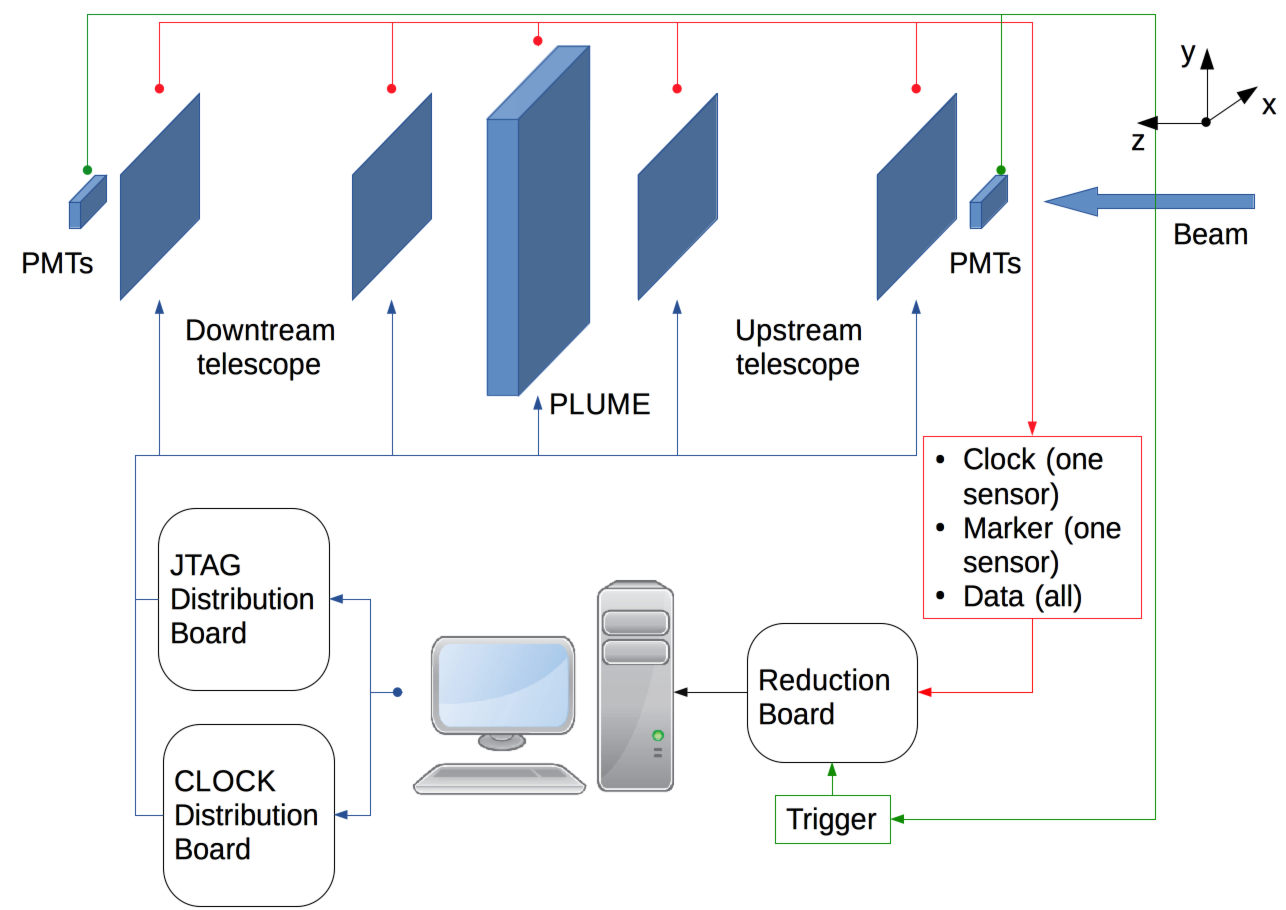
\includegraphics[width = \textwidth]{Pictures/X0/testBeamAcquisition.png}
      \caption{Schematic of the test beam set-up. The PMTs are used for triggering. The clock and marker are read from only one sensor, here it comes from one PLUME sensor.}
      \label{fig:testBeamAcq}
    \end{figure}

    \begin{figure}
      \centering
      \includegraphics[width = 0.8\textwidth]{Pictures/X0/testBeam.png}
      \caption{Picture taken during the test beam. The beam is going out of the magnet before to reach the four telescope planes, the DUT and the PMTs. The set-up is mounted on a floating frame insuring the grounded.}
      \label{fig:testBeam}
    \end{figure}

   
  \section{Measuring the radiation length}

    \subsection{Introduction}
    
    When charged particles are traveling through matter, they lose energy via inelastic collision with atomic electrons and this leads to the ionisation or excitation of the matter.
    Furthermore, along their path, they are deflected by many small angles from their initial trajectory due to Coulomb scattering from nuclei. 
    This stochastic effect, called multiple Coulomb scattering, leaves on the average the particle undisturbed through its path. 
    For small angles of deviation, the multiple scattering is following a Gaussian behavior, whereas for larger angles, it behaves like the Rutherford scattering.
    The Highland formula, which is an empirical formula, describes the distribution of the multiple scattering, or the "kink angle" as a function of the momentum $p$ of the incoming charge particles, its velocity $\beta c$, its charge number $z$ and its true path length in radiation length unit $\frac{x}{X_{0}}$:

    \begin{equation}
      \theta_{0} = \frac{13.6~\rm{MeV}}{\beta c p} z \sqrt{\frac{x}{X_{0}}}\left(1 + 0.038 \ln{\frac{x}{X_{0}}}\right).
      \label{eq:Highland}
    \end{equation}

    For the electrons, a modified version of the equation~\ref{eq:Highland} describes its scattering better than the Highland formula\cite{GEANT4}.

    \begin{equation}
      \theta_{0} = \frac{13.6~\rm{MeV}}{p}\left(\frac{x}{X_{0}}\right)^{0.555},~\text{with $\beta c = 1$.}
    \end{equation}

    The spread angle $\theta_{0}$ depends on the momentum of the incoming particle, as well as the relative radiation length $\frac{x}{X_{0}}$.
    Thus, for a given relative radiation length, the kink angle is becoming smaller for higher momentum, and for a given momentum, this kink angle is not the same for different relative radiation lengths.

    \subsection{Motivation}

    The design of a detector is driven by its intrinsic characteristics, such as the pointing resolution or the integration time, but also by some requirements on the material budget.
    For example, the \gls{ILC} sets new goals for the design of the vertex detector, but also for other parts of the detector, as mentioned in chapters~\ref{chap:ILC} and~\ref{chap:vxd}.
    For such detector, the tracking system should detect precisely the particles path and minimise their energy degradation, while the calorimeters have to measure accurately the energy deposited by the particles.
    During the physics analysis, the reconstruction of the events depends strongly on the knowledge of the energy loss by the particles inside the different components of the detector before they reach the calorimeters. 
    To improve the results, a correction on the energy as to be applied.
    Thus, the study of the radiation length $\rm{X_{0}}$ in $\rm{g.cm}^{2}$, which is the amount of matter traversed by the electron is an important part of the detector development.
    For electrons and positrons, the radiation length corresponds to the mean distance over which these particles loss $1/e$ of its energy by bremsstrahlung.

    As detector are made of different layers, the radiation length for composite materials is given as:

    \begin{equation}
      \frac{1}{X_{0}} = \sum_{j} \frac{\omega_{j}}{X_{j}},
    \end{equation}

   where $\omega_{j}$ and $X_{j}$ are the fraction by weight and radiation length for the $j^{\rm{th}}$ element.


    \subsection{The DESY II test beam facility}

    The \gls{DESY} test beam facility is composed of three areas.
    Firstly, the electron beam is produced in the LINAC-II and accelerated up to 450 MeV before to be injected in the DESY-II synchrotron ring.
    The DESY-II is used as a storage ring for the PETRA-III accelerator. 
    The beam is accelerated and stored until enough particles are available to be sent on to PETRA, where they are used for photon science.
    
    \begin{figure}[!h]
      \centering
      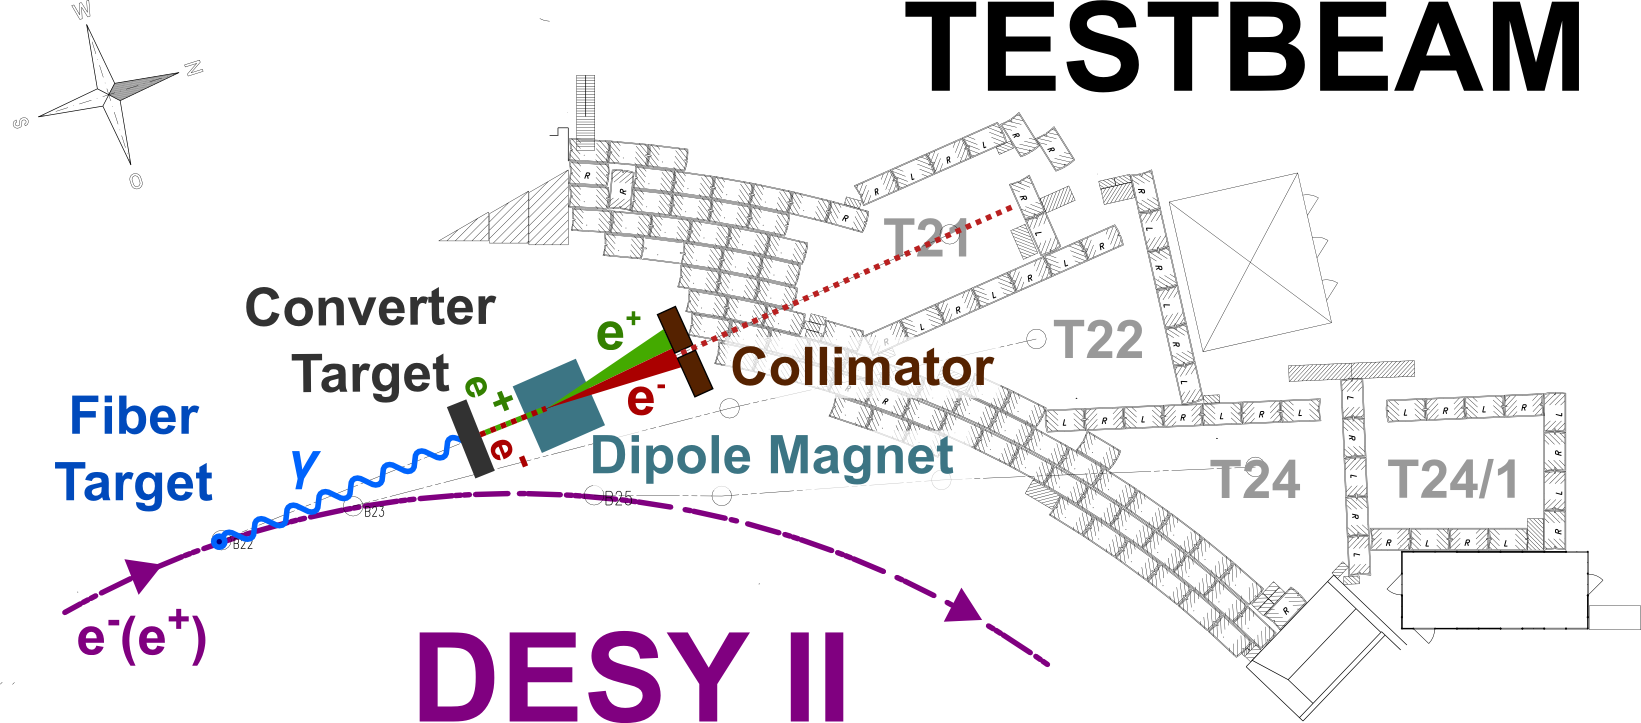
\includegraphics[width = 0.8\textwidth]{Pictures/X0/desy_tb-sketch.png}
      \caption{Schematic layout of the DESY-II test beam facility\cite{DESYII}.}
      \label{fig:desyTb-sketch}
    \end{figure}

    To generate the beam delivered in the Hall 26, a graphite fiber target is placed inside the beam pipe.
    While the electrons are hitting the target, they lose energy and emit bremsstrahlung photons.
    The photons travel through the air and hit another target, on which the photons are converted to pairs of electrons and positrons.
    Different targets with different thicknesses are available and this will impact the particles rate.
    One is made of copper, whereas the other one is made of aluminum.
    Then, a dipole magnet bends the particles and spread them according to their energy.
    Afterward, a tungsten collimator cuts away the unwanted particles, those having a too high or too low momentum, before the test beam area.
    A second collimator is located in the test beam area and it determines the size of the beam spot.
    The figure~\ref{fig:desyTb-sketch} summarises the different step to generate a beam of electrons or positrons in test beam 21, while the energies and the rates available are displayed in figure~\ref{fig:rateTB21}

    \begin{figure}[!h]
      \centering
      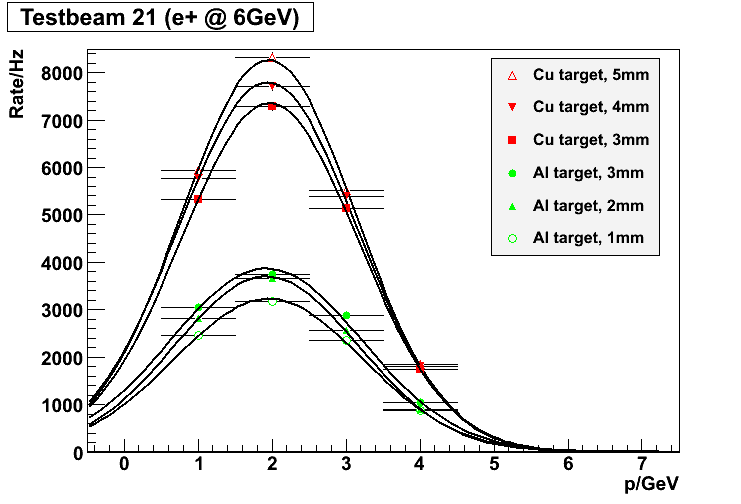
\includegraphics[width = 0.8\textwidth]{Pictures/X0/rate_vs_p_t21.png}
      \caption{Rate for different momentum and with different converter targets\cite{DESYII}.}
      \label{fig:rateTB21}
    \end{figure}


  \section{Analysis}
  \label{sec:X0}

   \subsection{Software analysis chain}

    The analysis of the test beam data is performed with EUTelescope\cite{Eutel}\cite{Jansen}.
    It is based on the MARLIN framework, which is a part of the ILCSOFT (see~\ref{subsec:ILCSOFT} for more details about the ILCSOFT package).
    The software is used to convert the data into the LCIO format and to perform clustering search, alignment and final analysis.
    Each step of the analysis is driven by a dedicated processor.

    A first processor is used to convert the raw data files acquired during the test beam into the LCIO format.
    The new file created contains the pixel number which fired in a given event, along with the sensor number.
    During the conversion, a hot pixel search is done to removed the noisy pixels from the list of hits.
    A pixel is considered as noisy if its firing frequency is above $0.001~\%$
    %From the raw data files, a first processor is used to convert the data into the LCIO format.
    %This converter file contains the pixel number which fired in a given event, along with the sensor number.
    %Before searching for clusters, the noisy pixels are removed from the list.
    %A pixel is considered as noisy if its firing frequency is above a certain value. 
    The noisy pixels correspond to defect raw or column or single pixels always sending information (see section~\ref{sec:noiseMeasurements}).
    Then, a cluster algorithm forms sets of cluster from the adjacent fired pixels in a row and/or column.
    Afterward, the hit candidates are defined with a centre-of-gravity method and the position of the hit is determined in the telescope frame and in the sensor frame.

    Although the alignment procedure looks like the one presented in chapter~\ref{chap:deformation}, the procedure used with EUTElescope is slightly different.
    The alignment is performed with \gls{GBL} and MILLEPEDE-II.
    In the case of a complete telescope (six planes), the tracks are built from the reconstruction of triplets in the upstream and downstream telescope planes.
    Firstly, a hit candidate from the outer plane is extrapolated by a straight line to the inner plane of one arm.
    Then, a triplet is formed if there is a matching between the middle plane of the arm and the doublet built.
    This is done on the two arms and a criterion ensures that two triplets are coming from the same track if the distance between the two extrapolated triplets at the middle $z$-position of the telescope is below a cut value.
    \gls{GBL} form a track from the six hits belonging to the matching triplets.
    The track candidates are then passed to MILLEPEDE-II, which determines the shift and the rotation to apply for aligning the sensors.
    This method is applied a couple of times, until the precision of the alignment reaches a submicron order.

    Nevertheless, due to the set-up used during the test beam and a limitation in EUTElescope on the number of telescope planes and the ID used, the alignment did not work.
    Indeed, the number of telescope planes is hard-coded to be six and the sensor IDs in the range $[0; 5]$ are reserved for the telescope. 
    Here, the IDS $0$ and $1$ are used for \gls{PLUME} and the others for the telescope.
    Thus, a modification has to be applied to remap the sensor IDs. 
    Although this solution can work and \gls{GBL} uses only the $z$ ordering information is used to create the tracks, EUTelescope is waiting for six hits.

   % For the upstream and the downstream plane, a hit position from the outer plane is projected on the inner plane with a straight line. 

   % Almost the same procedure as presented in chapter~\ref{chap:deformation} is performed, except that the alignment is done with \gls{GBL}.

   % Nevertheless, for my set-up, the alignment step did not work.
   % Inside EUTelescope, the number of telescope planes is hard-coded to be six and the sensor IDs in the range $[0; 5]$ are only for the telescope.
   % These IDs have to be ordered according to the $z$-direction too.
   % In my case, the IDs $0$ and $1$ are used for \gls{PLUME} and the rest for the telescope. 
   % Although \gls{GBL} uses only the $z$-ordering information to perform the alignment, the alignment procedure never worked.

    Thankfully, a prototype software developed by Claus Kleinwort has permitted to perform the alignment and finish the analysis. 
    It is based on \gls{GBL} and MILLEPEDE-II and reads the hit information created by the hitmaker processor of EUTelescope. 
    The modularity of the software allows to select the desire number of telescope planes.
    In the case of only four telescope planes, the triplets method is not used and tracks are formed only with doublets.
    Then, the track's information are feed to MILLEPEDE-II, which calculates the residuals of the tracks on each sensor and attempts to shift the position and rotate the sensors to minimise the east square fit function of these tracks.
    MILLEPEDE-II creates an output file with theses informations and a script update the GEAR file with the new position and orientation of each planes.

    %Then, the subtrack is extrapolated to the middle plane of the arm and \gls{GBL} is looking for the closest hit to the subtrack candidate.
    %This tracks are called triplets.
    %Afterward, the software finds if triplets are converging at the \gls{DUT} position and form a single track, unless multiple triplets are connected at the same position.
    %In this case, the track is rejected.

    %The tracks created are then read by Millepede-II, which calculates the residuals of the tracks on each sensor and attempts to shift the position of the sensors and to rotate them in order to minimise the least squares fit function of these tracks.
    %Millepede-II provides these informations into an output file used to create a new GEAR file with the new position and orientation of each plane.
    
    \begin{figure}[!h]
      \centering
      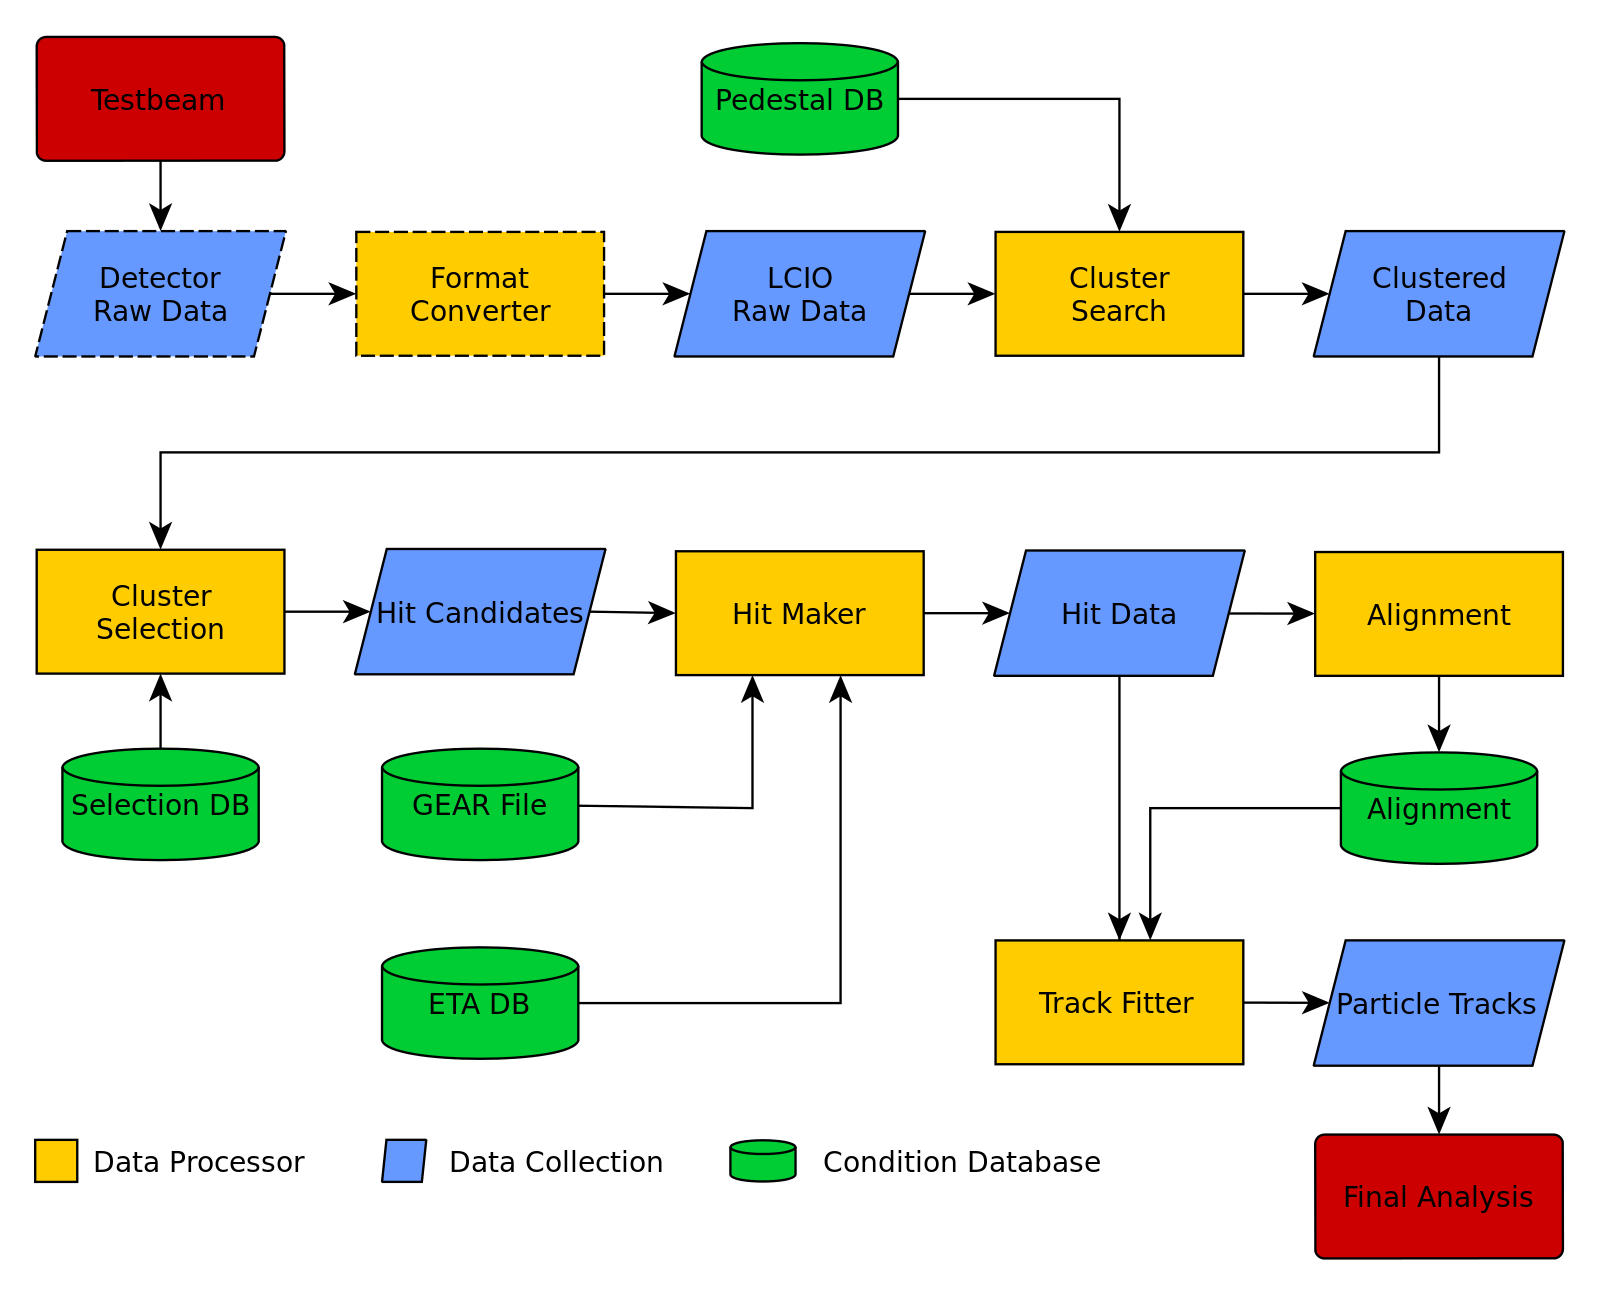
\includegraphics[width = \textwidth]{Pictures/X0/eutel-strategy.png}
      \caption{Flow-chart of the analysis strategy by using EUTelescope.}
      \label{fig:eutel-strategy}
    \end{figure}

   \subsection{Measurement of the radiation length}

   To extract the radiation length a biased alignment is performed.
   The hit information of \gls{PLUME} are used to create tracks by using the triplets method.
   The deviation of the track between its position before \gls{PLUME} and after \gls{PLUME} is measured with \gls{GBL}, that provides information for $xz$ and $yz$-angles.
   The distribution of the kink angle is fitted by a Gaussian, as represented on figure~\ref{fig:kinkAngle} for an energy of $5~\rm{GeV}$.
   The distribution displayed here is the kink angle measured on all the reference planes, no fiducial cut was applied. 

%
%   The extraction of the radiation length is done by measuring the kink angle between the track reconstructed before the \gls{DUT} and the track reconstructed after.
%   \gls{GBL} provides this information for $xz$ and $yz$-angles.
   %For the results presented here, a track is made of six hits: four coming from the telescope planes and two from the \gls{PLUME} sensors.
   %The distribution of the kink angle is fitted by a Gaussian, as represented on figure~\ref{fig:kinkAngle} for an energy of $5~\rm{GeV}$.
   Here, no fiducial cut has been applied and the measured kink angle is done on the overlapping region between the telescope and the \gls{DUT} planes.
   As it can be seen, the fit is not performed on the full range because of tails due to systematic errors.
   The measured kink angle is done for the energy range $[1; 5]~\rm{GeV}$ with a step of $1~\rm{GeV}$.
   The figure~\ref{fig:theta0vsP_all} displays the kink angle measured as a function of the particles momentum.
   The uncertainty on the momentum is $5~\%$ and is the uncertainty determined at the DESY test beam facility, while the uncertainty used for the kink angle is extracted from the fit procedure.
   The plot is then fitted with the Highland formula, on which the radiation length is a free parameter.
   The fit result is not convincing.
   Two points ($1$ and $5~\rm{GeV}$) are excluded and the $\chi^2 /~\rm{N.D.F}$ measured is bigger than $1$.
   Nevertheless, the $5~\rm{GeV}$ measurement gives a radiation length of $\sim 0.65~\%~\rm{X_{0}} $.

   During the alignment procedure, the runs at $1$ and $2~\rm{GeV}$ were complicated to be done.
   At those energies, the electron are more sensitive to the multiple scattering in the air and inside the detectors.
   By excluding the $1~\rm{and}~2~\rm{GeV}$ measurement, the radiation length is $x/X_0 \simeq 0.53~\%~\rm{X_{0}}$ and the $\chi^2$ is closer to one.

   %After the alignment step is done, the extraction of the radiation length from the reconstructed data can start.

   %Firstly, the angle between the track reconstructed by the upstream and the downstream telescope arms is studied.
   %\gls{GBL} is providing this information for $xz$ and $yz$-angles.
   %The distribution is fitted by a Gaussian, as seen on figure~\ref{fig:kinkAngle}.
   %As it can be seen, the fit is not performed on the full range because of tails due to systematic errors.
   %The measured kink angle is done for different energies to extract the radiation length.
   
   \begin{figure}
     \centering
     \missingfigure{Kink angle distribution}
     \caption{Distribution of the kink angle given by GBL for an energy of $5~\rm{GeV}$ without any fiducial cut.}
     \label{fig:kinkAngle}
   \end{figure} 

   %This measurement was performed at $5~\rm{GeV}$ and by using the Highland formula, the material budget determined is $\sim 0.6~\%~\rm{X_{0}} \pm $.

   %A sanity check is done for energies from 1 to $4~\rm{GeV}$.
   %The same procedure is applied and the distribution of the kink angle measured as a function of the momentum of the beam is plotted and fitted by the Highland formula to determine the radiation length of the \gls{DUT} (see~\ref{fig:theta0vsP}).
   %The uncertainty on the momentum is set to $5~\%$ and is the uncertainty measured at the DESY test beam facility, while the uncertainty used for the kink angle is extracted from the fit procedure.
   %Nonetheless, the fit results is bad and the measured radiation length is $x/X_0 \simeq 0.48~\%~\rm{X_{0}}$.
   %The measured radiation length is below the theoretical expectation but other tests have to be performed before to conclude.

   %The radiation length depends only on the material and not the energy.
   %Nevertheless, the figure~\ref{fig:X0vsP} which represents the measured radiation length as a function of the momentum, gives a $\rm{X_{0}}$ depending on the momentum.
   %So, the $0.53~\%~\rm{X_{0}}$ measured are likely to be wrong.

   %The error could emerge from the small analysis software to produce the plots.
   %To check the exactness of the code, the 

   \begin{figure}
     \centering
     \includegraphics[width = \textwidth]{Pictures/X0/theta0VsP_all.png}
     \caption{Extrapolation of the measured radiation length with a fit between 1 and 5 GeV.}
     \label{fig:theta0vsP_all}
   \end{figure}
   \begin{figure}
     \centering
     \includegraphics[width = \textwidth]{Pictures/X0/theta0VsP_3-5GeV.png}
     \caption{Extrapolation of the measured radiation length in the range 3 to 5 GeV.}
     \label{fig:theta0vsP_3-5}
   \end{figure}

   \begin{figure}
     \centering
     \missingfigure{x/X0 Vs energy}
     \label{fig:X0vsP}
   \end{figure}


  \section{Conclusions}

  The radiation length measurement of the \gls{PLUME} ladder was performed for the first time and the results are not good enough to conclude if the material budget determined theoretically for the first fully functional ladder is correct.
  To improve the measurement, it could be useful to perform calibration runs with a known material to check that the analysis is working correctly.
  Moreover, a correction can be performed then on the measured material budget with \gls{PLUME}.

  During the test beam and the data analysis, there was several problems.
  Firstly, due to a broken component on the power distribution board, one side of \gls{PLUME} was not working correctly.
  The sensors were sending the \textit{header} and \textit{trailer} but no data information, leading to two days of fully test before to find the origin of the problem.
  Fortunately, after replacing the broken component, the ladder was working normally but it is likely that the thresholds set were not correct anymore.
  Nevertheless, the data could have been corrupted and this should be investigated.

  Besides the analysis was complicated.
  EUTelescope is expecting a certain sensor IDs order and six telescope planes, even if \gls{GBL} is working from three to a huge amount of plane.


%	  

 %   %\chapter*{Conclusions}
\chapter*{Conclusions and outlooks\markboth{CONCLUSIONS AND OUTLOOKS}{CONCLUSIONS AND OUTLOOKS}} \addcontentsline{toc}{chapter}{\protect\numberline{}Conclusions and outlooks}

Over the last years, the scientific community agrees that an accelerator beyond the \gls{LHC} is needed.
This next generation accelerator is required for high-precision measurements, specifically for characterising the electroweak symmetry breaking, as well as looking for event compatible with physics beyond the \gls{SM}.
So far, the most advanced candidate is the \gls{ILC}.
With the technical design report~\cite{Baer2013}, the physicists have confirmed that the community is ready to build this future linear collider.
A governmental decision is eagerly awaited to start the project.
The work performed during this thesis was specifically focused on the feasibility to construct double-sided pixelated layers suited for a vertex detector at the \gls{ILC}, that features a low material budget (below $0.35~\%~\rm{X_{0}}$) and a spatial resolution below $\sim 3~\rm{\mu m}$ for the \gls{ILD}.

This work is introduced with a physics analysis on simulated data corresponding to collision in the \gls{ILC} at a centre-of-mass energy $\sqrt{s} = 350~\rm{GeV}$.
The channel studied underlines the benefits of event types produced by $e^{+}e^{-}$ collisions, it is the one leading to a $\nu \overline{\nu} H$ final state, with the Higgs boson decaying into pair of quarks or gluons.

The large part of the final particles produced in such events are invisible to the detector. 
Hence a corner stone of the analysis of this channel is the ability to drastically reduce the contribution of events leading to the same detector response or a similar event signature. 
The result presented in this work shows that applying a sequence of cuts on eight identified discriminating variables allows to reach a significance of 64 for the signal within the selected events. 
This level is however not sufficient for the precision measurement targeted with these events, which requires a significance of 70. 
Though sequential cuts are able to reduce by three orders of magnitude the background events, in the meantime they also remove half of the signal onces. 
To improve on our result, another thesis work conducted by Felix \textsc{Mueller}~\cite{Mueller} developed a multivariate analysis  approach, which finally reached the desired significance for the event selection process.

After this first important analysis step, actual characterization of the Higgs boson can start. 
But this second study was beyond the scope of this work even if it is strongly related to our goal. 
Indeed this characterization requires among others to identify jets issued from $c$ quark against those produced by $b$ quarks. 
This ability sets stringent specifications on the vertex detector layers, since the identification relies on the short lifetime difference between these two types of quarks. 
The \gls{PLUME} collaboration ambitions to demonstrate the feasibility of such layers, exploiting the concept of double-sided ladders.


%To reduce the contribution of events leading to the same detector response or a similar event signature, several hard cuts depending on different parameters are applied. 
%After eight cuts, the background events are three orders smaller but this method implies a lose of half of the signal.
%Due to the restricted time to conduct this work, a different selection technique could not be used.
%The work performed by Felix \textsc{Mueller} has nevertheless, shown that a TMVA solution will keep the signal significant while reducing the background contribution \cite{Mueller}.
%This analysis has to be completed with a study of the Higgs boson decaying into a pair of charmed and anti-charmed quarks.
%The ability of measuring the coupling of the Higgs boson to the $c$ quarks is needed. 
%This measurement is challenging to perform at the \gls{LHC} due to the \gls{QCD} background. 
%Moreover, the life-time of the $b$ and $c$ quarks are similar, leading to a close vertex decay. 
%Thus, the vertex detector has to be optimised to separate this two quarks.

The largest part of this thesis work was devoted to study \gls{PLUME} prototypes, which are currently equipped with \gls{CMOS} pixel sensors.
Since the first small scale prototype (V0) developed in 2009, the collaboration has shown its capability to build full scale and fully functional \gls{PLUME} ladders.
Two versions have been produced so far, the first one (V1) with a relaxed material budget constraint and the final one approaching the $0.3~\%$ of $\rm{X_{0}}$ requirement.
The work done during this three years was split into checking the basic assessments of individual \gls{PLUME} module before assembling them into ladders, studying the impact of the mechanical deformations on the pointing resolution and preparing a protocol to measure the radiation length of complete ladders.

The validation and characterisation of the final ladder done in laboratory have shown that the combination of six sensors running at the same time does not degrade the performances of the \gls{MIMOSA}-26.
The fake hit rate measured for the different modules is below 

During the data analysis of the test beam performed in 2011 at \gls{CERN} with the V1 ladder, runs where the ladder was tilted with respect to the track direction have shown deviation on the pointing resolution, as well as a correlation between the position of the hit on the sensor and the track residual measured.
These deviations are coming from mechanical deformation induced by the material used (flex-cable, foam) during the mounting procedure of a \gls{PLUME} ladder.
An algorithm to reduce the impact of these deformations have been implemented and has shown a good improvement on the pointing resolution measured for titled tracks.
A second study during this data analysis has permitted to present the benefits of a double-sided measurement. 
The spatial resolution has been improve by a factor of about $1/\sqrt{2}$ and the creation of mini-vectors give access to a new parameter, the angular resolution, which was measured to be $0.1^{\circ}$ at normal incidence.

Finally, the last work performed during the thesis was to set-up a test beam with a lower beam energy (up to $5~\rm{GeV}$ electrons) to measure the radiation length of the first fully functional prototype.
After analysing the data, the radiation length measured is $\left. \frac{x}{X_0} \right|_{\rm{measured}} \simeq 0.47 \pm 0.02~\%~\rm{X_0}$, confirming the theoretical calculation of $\left. \frac{x}{X_0}\right|_{\rm{theoretical}} \simeq 0.498~~\%~\rm{X_0}$.
This measurement is in a good agreement to the theoretical value determined, even if the measured value is a bit lower than the expectations. 
To improve the precision on the measurements, different methods could be used.
Instead of using the \gls{PLUME} sensors as reference planes, the six telescope planes could be used to measured the deflection of the complete ladder.

% OUTLOOKS:
%  * Test beam at low energy
%    - Efficiency and resolution?
%  * Power-pulsing
%    - Mi-26?
%    - Magnetic field?
%  * New structure
%    - Sernwiette? 

The work performed during this thesis has shown that the collaboration is able to build lightweight mechanical structure for a vertex detector.
The material budget has been controlled and the first results are encouraging, a way to overcome the mechanical deformation inherent to the thin-sensor concept have been discussed.
Moreover, this thesis, as well as the work performed by Loic \textit{Cousin} and Robert \textit{Maria}, have shown that \gls{CMOS} sensors are disturbed when they are closely laid together (butted and facing each others), but the expected performances (efficiency and spatial resolution) for one sensor are measured for a ladder.
Nevertheless, the new ladder prototype with a material budget of $0.35~\%$ of $\rm{X_{0}}$ has not been tested in real conditions yet.



Nevertheless, more tests and optimisations have to be done to improve the ladder.

Firstly, the results of the test beam performed in April 2016 presented here are focused only on the material budget measurement.
The performances of the ladder (efficiency and spatial resolution) for low momentum particles have to be checked.
Runs with different tilts and air flow speed were acquired in order to study the mechanical deformations in more details.

Secondly, the sensors used for validating the mechanical structure are \gls{MIMOSA}-26.
They have the advantage of having a continuous readout without suffering from dead time, but their integration time is rather slow ($115.2~\rm{\mu s}$).
This imposes to readout the data between two bunch crossings at the \gls{ILC}.
But to keep the material budget below $1.5~\%~\rm{X_{0}}$, the power consumption of the sensors have to be adapted to the cooling system used.
One way to decrease the power consumption is to use a \textit{power-pulsing} solution.
This consists to reduce the consumption of the sensors during the $200~\rm{ms}$ of dead time and switching them on before the bunch crossing.
Tests to perform \textit{power-pulsing} on a single \gls{MIMOSA}-26 sensor have been performed by the collaboration.
The results have shown that the nominal supply voltage can de decreased from $3.3~\rm{V}$ to $1.85~\rm{V}$ without losing the sensor's registers~\cite{Kuprash2013}.
Nonetheless, this sensor is not designed for this purpose and its behavior with other sensors inside a complete ladder is not known yet.
Different tests have to be done to make sure that the ladder is still behaving correctly in a \textit{power-pulsing} mode.
If the results are comforting, the ladder have to be then tested under real conditions with a high magnetic field (ideally $3~\rm{T}$).
This tests is needed to study the impact of the Lorentz forces on the whole ladder, especially to know if it induces unwanted deformations or vibrations of the ladder.

Finally, the mechanical structure can be improved by embedding the sensors directly inside the multi-lay micro-cable~\cite{Baudot2012}.
This technique consists to glue the chips on a first polymide substrate layer.
Then, a metal layer is deposited on top of it and the metal traces are directly connected to the chips pads.
On the last step, an insulator is added to the module.
This method offers the advantage of avoiding the wire-bonding and reducing in the same time the width of the module.
Moreover, with this structure, mechanical stress is applied on the polymer wrapping and reducing its impact on the sensors.
The advantages of this technique are the ability to connect directly the metal traces to the pads, avoiding wire-bonding and reducing in the same time the width of the module.


%	  \appendix	  
    
 %   \backmatter

	
  \printglossary[type=\acronymtype]
  
  \bibliographystyle{plain}
	\bibliography{Bibliography/biblio}


\end{document}

